\documentclass[]{book}
\usepackage{lmodern}
\usepackage{amssymb,amsmath}
\usepackage{ifxetex,ifluatex}
\usepackage{fixltx2e} % provides \textsubscript
\ifnum 0\ifxetex 1\fi\ifluatex 1\fi=0 % if pdftex
  \usepackage[T1]{fontenc}
  \usepackage[utf8]{inputenc}
\else % if luatex or xelatex
  \ifxetex
    \usepackage{mathspec}
  \else
    \usepackage{fontspec}
  \fi
  \defaultfontfeatures{Ligatures=TeX,Scale=MatchLowercase}
\fi
% use upquote if available, for straight quotes in verbatim environments
\IfFileExists{upquote.sty}{\usepackage{upquote}}{}
% use microtype if available
\IfFileExists{microtype.sty}{%
\usepackage{microtype}
\UseMicrotypeSet[protrusion]{basicmath} % disable protrusion for tt fonts
}{}
\usepackage{hyperref}
\hypersetup{unicode=true,
            pdftitle={e-Business},
            pdfauthor={Robert Batzinger},
            pdfborder={0 0 0},
            breaklinks=true}
\urlstyle{same}  % don't use monospace font for urls
\usepackage{natbib}
\bibliographystyle{alpha}
\usepackage{color}
\usepackage{fancyvrb}
\newcommand{\VerbBar}{|}
\newcommand{\VERB}{\Verb[commandchars=\\\{\}]}
\DefineVerbatimEnvironment{Highlighting}{Verbatim}{commandchars=\\\{\}}
% Add ',fontsize=\small' for more characters per line
\usepackage{framed}
\definecolor{shadecolor}{RGB}{248,248,248}
\newenvironment{Shaded}{\begin{snugshade}}{\end{snugshade}}
\newcommand{\AlertTok}[1]{\textcolor[rgb]{0.94,0.16,0.16}{#1}}
\newcommand{\AnnotationTok}[1]{\textcolor[rgb]{0.56,0.35,0.01}{\textbf{\textit{#1}}}}
\newcommand{\AttributeTok}[1]{\textcolor[rgb]{0.77,0.63,0.00}{#1}}
\newcommand{\BaseNTok}[1]{\textcolor[rgb]{0.00,0.00,0.81}{#1}}
\newcommand{\BuiltInTok}[1]{#1}
\newcommand{\CharTok}[1]{\textcolor[rgb]{0.31,0.60,0.02}{#1}}
\newcommand{\CommentTok}[1]{\textcolor[rgb]{0.56,0.35,0.01}{\textit{#1}}}
\newcommand{\CommentVarTok}[1]{\textcolor[rgb]{0.56,0.35,0.01}{\textbf{\textit{#1}}}}
\newcommand{\ConstantTok}[1]{\textcolor[rgb]{0.00,0.00,0.00}{#1}}
\newcommand{\ControlFlowTok}[1]{\textcolor[rgb]{0.13,0.29,0.53}{\textbf{#1}}}
\newcommand{\DataTypeTok}[1]{\textcolor[rgb]{0.13,0.29,0.53}{#1}}
\newcommand{\DecValTok}[1]{\textcolor[rgb]{0.00,0.00,0.81}{#1}}
\newcommand{\DocumentationTok}[1]{\textcolor[rgb]{0.56,0.35,0.01}{\textbf{\textit{#1}}}}
\newcommand{\ErrorTok}[1]{\textcolor[rgb]{0.64,0.00,0.00}{\textbf{#1}}}
\newcommand{\ExtensionTok}[1]{#1}
\newcommand{\FloatTok}[1]{\textcolor[rgb]{0.00,0.00,0.81}{#1}}
\newcommand{\FunctionTok}[1]{\textcolor[rgb]{0.00,0.00,0.00}{#1}}
\newcommand{\ImportTok}[1]{#1}
\newcommand{\InformationTok}[1]{\textcolor[rgb]{0.56,0.35,0.01}{\textbf{\textit{#1}}}}
\newcommand{\KeywordTok}[1]{\textcolor[rgb]{0.13,0.29,0.53}{\textbf{#1}}}
\newcommand{\NormalTok}[1]{#1}
\newcommand{\OperatorTok}[1]{\textcolor[rgb]{0.81,0.36,0.00}{\textbf{#1}}}
\newcommand{\OtherTok}[1]{\textcolor[rgb]{0.56,0.35,0.01}{#1}}
\newcommand{\PreprocessorTok}[1]{\textcolor[rgb]{0.56,0.35,0.01}{\textit{#1}}}
\newcommand{\RegionMarkerTok}[1]{#1}
\newcommand{\SpecialCharTok}[1]{\textcolor[rgb]{0.00,0.00,0.00}{#1}}
\newcommand{\SpecialStringTok}[1]{\textcolor[rgb]{0.31,0.60,0.02}{#1}}
\newcommand{\StringTok}[1]{\textcolor[rgb]{0.31,0.60,0.02}{#1}}
\newcommand{\VariableTok}[1]{\textcolor[rgb]{0.00,0.00,0.00}{#1}}
\newcommand{\VerbatimStringTok}[1]{\textcolor[rgb]{0.31,0.60,0.02}{#1}}
\newcommand{\WarningTok}[1]{\textcolor[rgb]{0.56,0.35,0.01}{\textbf{\textit{#1}}}}
\usepackage{longtable,booktabs}
\usepackage{graphicx,grffile}
\makeatletter
\def\maxwidth{\ifdim\Gin@nat@width>\linewidth\linewidth\else\Gin@nat@width\fi}
\def\maxheight{\ifdim\Gin@nat@height>\textheight\textheight\else\Gin@nat@height\fi}
\makeatother
% Scale images if necessary, so that they will not overflow the page
% margins by default, and it is still possible to overwrite the defaults
% using explicit options in \includegraphics[width, height, ...]{}
\setkeys{Gin}{width=\maxwidth,height=\maxheight,keepaspectratio}
\IfFileExists{parskip.sty}{%
\usepackage{parskip}
}{% else
\setlength{\parindent}{0pt}
\setlength{\parskip}{6pt plus 2pt minus 1pt}
}
\setlength{\emergencystretch}{3em}  % prevent overfull lines
\providecommand{\tightlist}{%
  \setlength{\itemsep}{0pt}\setlength{\parskip}{0pt}}
\setcounter{secnumdepth}{5}
% Redefines (sub)paragraphs to behave more like sections
\ifx\paragraph\undefined\else
\let\oldparagraph\paragraph
\renewcommand{\paragraph}[1]{\oldparagraph{#1}\mbox{}}
\fi
\ifx\subparagraph\undefined\else
\let\oldsubparagraph\subparagraph
\renewcommand{\subparagraph}[1]{\oldsubparagraph{#1}\mbox{}}
\fi

%%% Use protect on footnotes to avoid problems with footnotes in titles
\let\rmarkdownfootnote\footnote%
\def\footnote{\protect\rmarkdownfootnote}

%%% Change title format to be more compact
\usepackage{titling}

% Create subtitle command for use in maketitle
\providecommand{\subtitle}[1]{
  \posttitle{
    \begin{center}\large#1\end{center}
    }
}

\setlength{\droptitle}{-2em}

  \title{e-Business}
    \pretitle{\vspace{\droptitle}\centering\huge}
  \posttitle{\par}
    \author{Robert Batzinger}
    \preauthor{\centering\large\emph}
  \postauthor{\par}
      \predate{\centering\large\emph}
  \postdate{\par}
    \date{2019-06-22}

\usepackage{booktabs}
\usepackage{amsthm}
\usepackage{graphicx}

\makeatletter
\def\thm@space@setup{%
  \thm@preskip=8pt plus 2pt minus 4pt
  \thm@postskip=\thm@preskip
}
\makeatother
\newenvironment{rmdexercise}{$$\begin{minipage}[t]{1cm}\vbox to 0pt{\null\kern 5pt\hbox{
\includegraphics[width=1cm]{images/checklist.png}}\vss}\end{minipage}\quad
   \begin{minipage}[t]{4.25in}\hrule\smallskip\small}{\smallskip\hrule\end{minipage}$$}
\newenvironment{rmdextra}{$$\begin{minipage}[t]{1cm}\vbox to 0pt{\null\kern 5pt\hbox{
\includegraphics[width=1cm]{images/study.png}}\vss}\end{minipage}\quad
   \begin{minipage}[t]{4.25in}\hrule\smallskip\small}{\smallskip\hrule\end{minipage}$$}
\newenvironment{rmddiscussion}{$$\begin{minipage}[t]{1cm}\vbox to 0pt{\null\kern 5pt\hbox{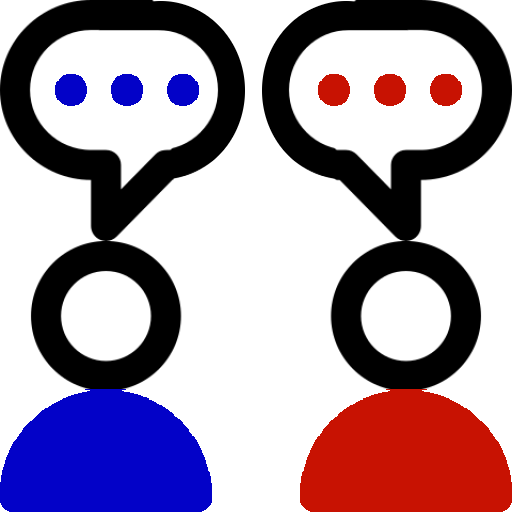
\includegraphics[width=1cm]{images/discuss.png}}\vss}\end{minipage}\quad
   \begin{minipage}[t]{4.25in}\hrule\smallskip\small}{\smallskip\hrule\end{minipage}$$}

\let\oldmaketitle\maketitle
\AtBeginDocument{\let\maketitle\relax}

\let\BeginKnitrBlock\begin \let\EndKnitrBlock\end
\begin{document}
\maketitle

\thispagestyle{empty}
\vbox to 10pt{\null
  \hsize=6in
  \kern -1in
\hrule
$$\hbox to 3in{\hss
\includegraphics[width=8in]{images/cover11.png}\hss}$$
\hrule height 10pt
\vss}
\frontmatter
\let\maketitle\oldmaketitle
\maketitle

{
\setcounter{tocdepth}{1}
\tableofcontents
}
\hypertarget{book-jacket}{%
\chapter*{Book Jacket}\label{book-jacket}}
\addcontentsline{toc}{chapter}{Book Jacket}


\includegraphics[width=0.5\linewidth]{images/cover11}

\hypertarget{abstract}{%
\section*{Abstract}\label{abstract}}
\addcontentsline{toc}{section}{Abstract}

This book attempts to introduce undergraduate students to the nature and requirements for conducting business online. It starts with a discussion of the nature of business and the challenges and potential of the online environment, followed by a review of common methods of modelling business, and a study of open source business solutions.
The final chapter focuses on emerging trends and sea-changes in e-Business. This book is currently a work in progress that is also comparing the process of book writing in both LeanPub markdown and Rstudio Bookdown

\hypertarget{about-the-author}{%
\section*{About the Author}\label{about-the-author}}
\addcontentsline{toc}{section}{About the Author}

Robert Batzinger is an emeritus instructor in Computer Science at Payap University. He holds an undergraduate degree in Organic Chemistry, masters degree in Computer Science and Applied Mathematics, doctoral degree in Pathobiology and post-doctoral training in Chemical carcinogenesis. As such, he has been involved in numerous scientific and technical projects for over 50 years. He has published laboratory research in such fields as virology, organic chemistry, anthelmithics, and chemical mutagenesis. He also developed software to manage the financial and academic records of schools, support the development of publications in non-Roman scripts of Asia and Canada, and monitor the progress of multiple development projects. He has held administrative and advisory roles in various organizations and businesses, and has been instrumental in establishing web presence for many of them. He is currently developing data science and machine learning applications to address critical business management problems.

\hypertarget{front-matter}{%
\chapter*{Front Matter}\label{front-matter}}
\addcontentsline{toc}{chapter}{Front Matter}

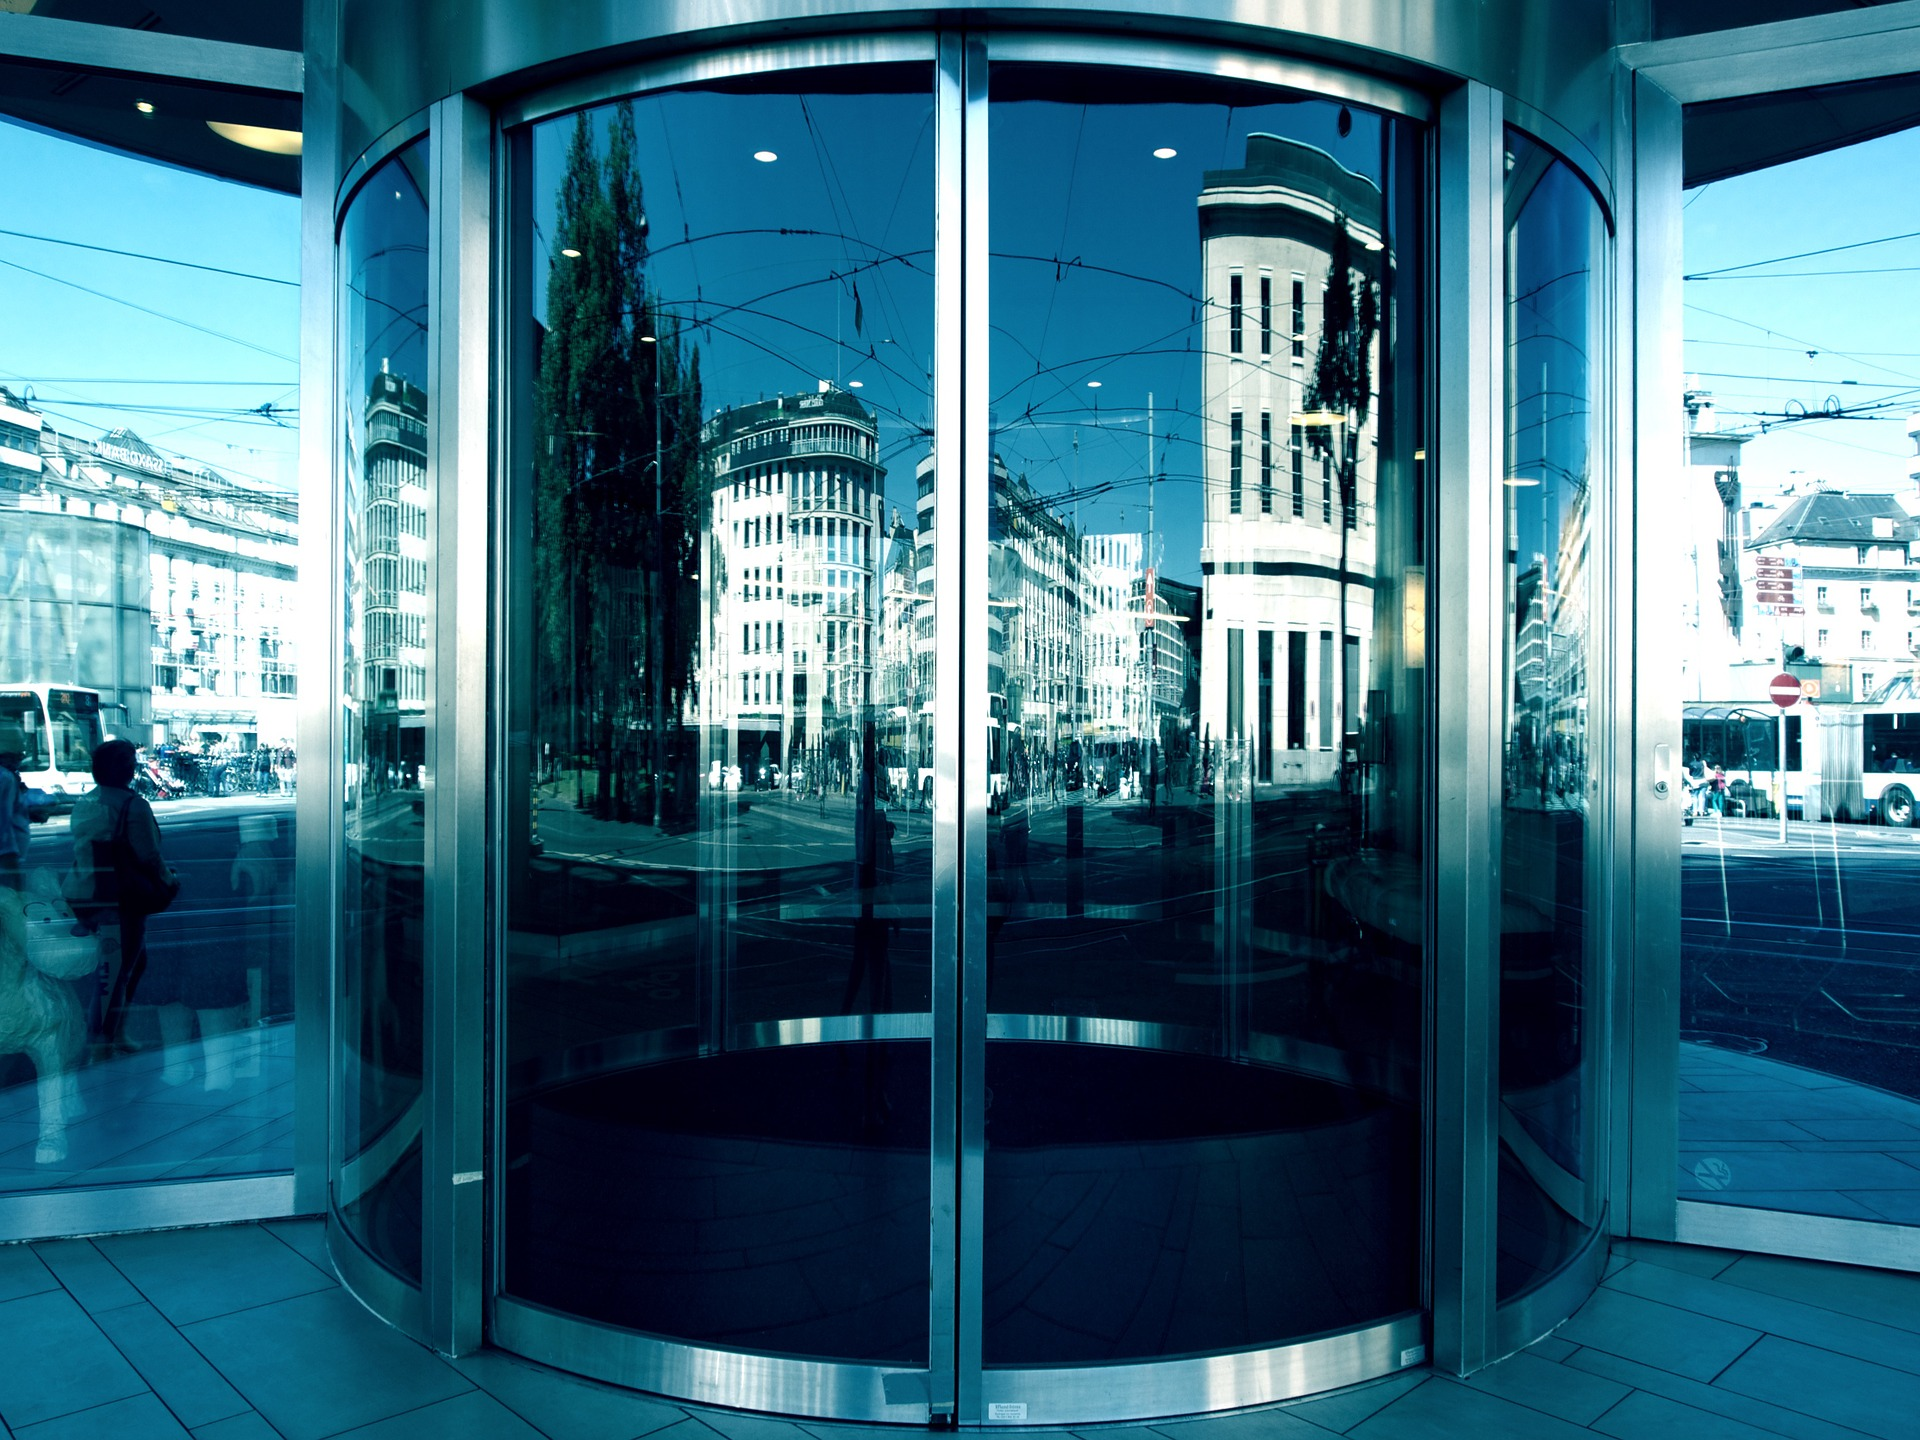
\includegraphics[width=0.9\linewidth]{images/door}

\hypertarget{dedication}{%
\section*{Dedication}\label{dedication}}
\addcontentsline{toc}{section}{Dedication}

\begin{quote}
Now to him who is able to do far more abundantly
than all that we ask or think, according
to the power at work within us.
-- Eph 3:20 (ESV)

ขอให้พระเกียรติมีแด่พระองค์ผู้ทรงสามารถทำทุกสิ่งได้
มากยิ่งกว่าที่เราทูลขอหรือคิด โดยฤทธานุภาพ
ที่ทำกิจอยู่ภายในเรา
-- เอเฟซัส 3:20 (THSV11)
\end{quote}

\hypertarget{acknowledgements}{%
\section*{Acknowledgements}\label{acknowledgements}}
\addcontentsline{toc}{section}{Acknowledgements}

The development of this book would not have been possible without the feedback and suggestions of colleagues and students. While I acknowledge that I am responsible for any remaining errors in this book, my students, referees, and readers have contributed immensely to the development of this book. I would like to acknowledge the impact of Ms.~Phatnaree Srisomphan in helping to shape both the curriculum of this course and the nature of this book. I am also grateful for the support and encouragement of my wife Khajohn, especially in those long critical sessions when I was struggling to forge and edit the text of this manuscript.

\hypertarget{colophon}{%
\section*{Colophon}\label{colophon}}
\addcontentsline{toc}{section}{Colophon}

The cover is a photograph of the Financial District from the Marina Bay in Singapore. The amazing metamorphsis of this central business district from swamp land into a thriving financial center of the Region is representative of the current sea-changes in business driven by technological and social developments. Similarly, today's developers of business systems are sowing seeds that will change the future, much like Sir Raffles' vision for a seaport has grown into today's Singapore.

While early drafts of this book were written in Leanpub Flavored Markdown, this book was developed in RStudio using the \textbf{bookdown} package \citep{R-bookdown} (which was built on top of R Markdown and \textbf{knitr} \citep{Xie2015}. It was edited in RStudio and later compiled and published online simultaneously as an HTML website, a printable document in PDF and electronic book EPUB format with only 3 clicks of the mouse.

The cover and front matter photos were downloaded from \href{https://pixabay.com/images/search/singapore}{Pixabay}.
The extra reading, discussion and exercise sidebar icons were created by \href{https://www.freepik.com}{Freepik} and used as per \href{https://creativecommons.org/licenses/by/3.0}{Creative Commons 3.0 License}.

\hypertarget{preface}{%
\chapter*{Preface}\label{preface}}
\addcontentsline{toc}{chapter}{Preface}

Advances and developments in Computer Science (CS) are driven by the need to create applications that effectively address real-world problems. Successful software development starts with a deep understanding of the problem domain from the users perspective and developing an application that is intuitive and easy to use. Breakthroughs in understanding the nature of a problem domain create new opportunities for addressing the needs of computer users. It is now common practice to integrate end users into software development and testing teams, as the resulting products tend to be more intuitive and successful.

In CS, our graduates will go on to develop applications and solutions for clients who, for the most part, have not studied CS, but who are experts in other problem domains. Courses that help students to explore and understand the basic issues in other problem domains are at the heart of our liberal arts education which balances professional skills with general knowledge needed to function effectively in the market place.
As a part of this effort to introduce CS students to e-Business from a Business/IT perspective, we offer a course with the following course description. It is taught in Thai using English-based resources.

\begin{quote}
\textbf{CS340 ธุรกิจอิเล็กทรอนิกส์:} หลักการการดำเนินธุรกิจโดยใช้สื่ออิเล็กทรอนิกส์ การวางแผนทรัพยากรขององค์กร การบริหารความสัมพันธ์ลูกค้า และการสื่อสารผ่านโซเชียลมีเดียทั้งภายในและภายนอกองค์กร
\end{quote}

\begin{quote}
\textbf{CS340 E-BUSINESS:} Principles of business operations using information technology. This includes a discussion of Enterprise Resource Planning (ERP), Customer Relationship Management (CRM) and the use of social media to communicate both within and outside the organization.
\end{quote}

This book is the product of that course and started as a collection of class slides, notes, and exercises. The content of this book continues to evolve in response to student feedback as well as changes in the software industry and conversations with business leaders and software developers. The basic design of this book is meant to parallel the outline of the corresponding course, as given below:

\begin{quote}
\textbf{Chapter 1: General principles.} A discussion of the key principles that define and characterize business both in the real world and in cyberspace.
\end{quote}

\begin{quote}
\textbf{Chapter 2: Business modeling.} A discussion of leading methods used to create software models of the key transactions and activities that take place in business in general and in e-business in particular.
\end{quote}

\begin{quote}
\textbf{Chapter 3: e-Business systems.} A survey of the concepts and functions of key open-source, online business systems. Each system is studied to determine how solutions are provided by addressing mission-critical questions using available data resources.
\end{quote}

\begin{quote}
\textbf{Chapter 4: Emerging Technologies.} A discussion of futuristic e-Business technologies and practices that have already had an impact on how business is conducted worldwide.
\end{quote}

\mainmatter

\hypertarget{general-principles}{%
\chapter{GENERAL PRINCIPLES}\label{general-principles}}

\begin{figure}
\centering
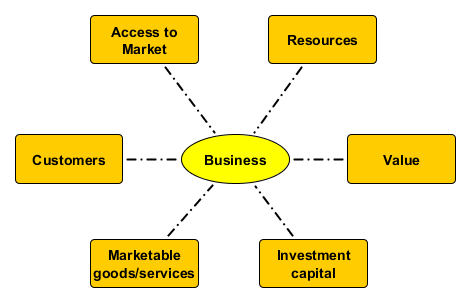
\includegraphics{images/keycomponents.png}
\caption{Key components of a thriving business}
\end{figure}

\hypertarget{essentials-of-business}{%
\section{Essentials of Business}\label{essentials-of-business}}

Business is a set of interactions in which goods and services are provided and compensation is rendered. Businesses become sustainable when the compensation rendered meets the short-term and long-term requirements of the business. Most business fail because of an inability to develop a network of processes and transactions to address a market demand that meets or exceeds their expenses. Ideally, a start-up should aim to seek fair compensation for goods and services rendered in the most effective and efficient manner.

\BeginKnitrBlock{rmdexercise}
\textbf{Exercise: The Nature of Business}

Discuss how the following premises would impact the nature, as well as the potential for long-term success of businesses.

\begin{enumerate}
\def\labelenumi{\arabic{enumi}.}
\tightlist
\item
  Business is all about making lots and lots of money quickly by any means possible.
\item
  Business is about fair compensation for goods and service to both suppliers and customers.
\item
  Business is the process of copying the industry leaders to provide similar goods and services at a fraction of the cost.
\item
  Business provides special opportunities for myself, my friends and relatives at the expense of our customers.
\end{enumerate}
\EndKnitrBlock{rmdexercise}

\hypertarget{business-processes}{%
\subsection{Business processes}\label{business-processes}}

Individual businesses are always centered around a core set of goods and services which address the specific needs of clients creating a sense of value and desire. Good design and pre-market testing help to define the nature of the products and services. At the same time, controlling production and distribution costs make it possible to deliver goods and services at a suitable price point for customers. Careful supply chain and operations management develops a network of contracts and business transactions with suppliers and distributors ensures that products and services are delivered on time and on budget.

\begin{figure}
\centering
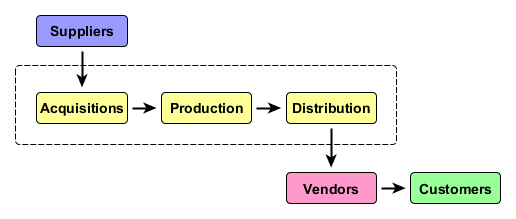
\includegraphics{images/businessprocess.png}
\caption{Key Business Processes}
\end{figure}

\BeginKnitrBlock{rmdexercise}
\textbf{Exercise: Match market principles to market characteristics}

\begin{longtable}[]{@{}ll@{}}
\toprule
\begin{minipage}[b]{0.44\columnwidth}\raggedright
Principles\strut
\end{minipage} & \begin{minipage}[b]{0.50\columnwidth}\raggedright
Characteristics\strut
\end{minipage}\tabularnewline
\midrule
\endhead
\begin{minipage}[t]{0.44\columnwidth}\raggedright
(A) Access to market \newline(B) Brand recognition\newline (C) Customer pool\newline(D) Investment capital\newline(E) Resources\newline(F) Market value\strut
\end{minipage} & \begin{minipage}[t]{0.50\columnwidth}\raggedright
\_\_\_ Consumer preference\newline  \_\_\_ Supply of raw materials\newline \_\_\_ Distinctive goods and services\newline\_\_\_ Investors and stock holders\newline \_\_\_ Location and traffic\newline\_\_\_ Steady market demand\strut
\end{minipage}\tabularnewline
\bottomrule
\end{longtable}
\EndKnitrBlock{rmdexercise}

\hypertarget{core-activities-of-a-business}{%
\subsection{Core Activities of a Business}\label{core-activities-of-a-business}}

Business requires coordinated teamwork of specialists in various departments to achieve efficiency and effectiveness on a large scale.

\begin{itemize}
\tightlist
\item
  \textbf{Finance:} mid-term and long-range financial planning to ensure that there is an adequate supply of money available to
\item
  \textbf{Accounting:} a record of financial commitments and compensations for the purpose of tracking movement of value across the organization and throughout the production process
\item
  \textbf{Marketing:} getting groups of potential customers and consumers interested in products and services.
\item
  \textbf{Sales:} selling products and services to customers maintain records to assist forecasting future demand and market growth
\item
  \textbf{Operations:} systems to acquire resources, produce, package and deliver products
\item
  \textbf{Management:} sets the direction and pace of business endeavors
\end{itemize}

\hypertarget{support-functions}{%
\subsection{Support functions}\label{support-functions}}

As businesses grow in size, various support functions are required to keep the core business running. These functions include the following:

\begin{itemize}
\tightlist
\item
  \textbf{Management Information Systems:} collect, analyze and distribute mission-critical information to key administrators
\item
  \textbf{Human Resources:} attract, hire, train and retain effective employees
\item
  \textbf{Legal Department:} ensure compliance with laws and regulations
\item
  \textbf{Investor Relations:} communications with shareholders to attract support and investments
\item
  \textbf{Customer Relations:} after sales care of customers and encouragement of brand loyalty
\item
  \textbf{Facilities Management:} maintenance of facilities and equipment to maximize the utility and value of capital investments in equipment and infrastructure.
\end{itemize}

\BeginKnitrBlock{rmdexercise}
\textbf{Exercise: Key business concepts}

Create a mindmap that illustrates the relationship between the following sets of terms, along with their Thai translations.

\begin{itemize}
\tightlist
\item
  \textbf{Key business components:} Access to market; Resources; Value; Investment capital; Marketable goods and services; Customers
\item
  \textbf{Core business activities:} Finance; Accounting; Marketing; Sales; Operations; Management.
\item
  \textbf{Support functions:} Management information systems; Human resources; Legal department; Investor relations; Customer relations; Facilities management
\end{itemize}
\EndKnitrBlock{rmdexercise}

\hypertarget{understanding-the-role-of-it-in-business}{%
\section{Understanding the role of IT in business}\label{understanding-the-role-of-it-in-business}}

As IT Departments become integrated into the business strategy, they provide tools, information and communication systems that can play a transformative role in the nature of the business. Enterprise Architecture tend to grow as IT Department move along these evolutionary steps. \citep{Hohpe2017a}, \citep{Hohpe2017b}

\hypertarget{the-establishment-of-an-it-department}{%
\subsection{The Establishment of an IT Department}\label{the-establishment-of-an-it-department}}

\begin{enumerate}
\def\labelenumi{\arabic{enumi}.}
\tightlist
\item
  Understand the business strategy
\item
  Translate into an IT strategy
\item
  Create transparency for IT developments
\item
  Define IT target picture
\item
  Define the roadmap for implementing IT
\item
  Harmonize and govern
\item
  Obtain feedback and refine
\item
  Coach and mentor
\end{enumerate}

Among IT Managers, there appears to be 2 major approaches to understanding the nature of business and IT's function: using IT to redesign the business or engineering the current organization. The political implications of the approach chosen can be immense and often the success of an IT manager will depend on the level of support from those that manage the IT department manager.

\begin{longtable}[]{@{}ll@{}}
\toprule
Architecting the Business & Reverse-Engineering the Organization\tabularnewline
\midrule
\endhead
* Identification of growth areas & * Divisions and business lines\tabularnewline
* Profitability of goods and services & * Group level vs divisions\tabularnewline
* Geographic/demographic opportunities & * Reportings lines\tabularnewline
* Geopolitical aspects & * Matrix organizations\tabularnewline
* Acquisitions and divestitures & * Hidden org chart/loyalties\tabularnewline
\bottomrule
\end{longtable}

\hypertarget{business-views-of-the-role-of-it}{%
\subsection{Business views of the role of IT}\label{business-views-of-the-role-of-it}}

Business managers have 4 main approaches to managing IT based on the main focus of the business administration.

\begin{longtable}[]{@{}rcclc@{}}
\toprule
\textbf{Focus} & \textbf{Role} & \textbf{Reports to} & \textbf{Common stragegy} & \textbf{Levers}\tabularnewline
\midrule
\endhead
Cost of IT & Cost Center & CFO & Outsource IT & Cost cutting\tabularnewline
Return on investment & Asset & COO & Harmonize / Rationalize & Economies of scale\tabularnewline
Business value of IT & Partner & CDO & Insource IT & Economies of Efficiency\tabularnewline
Speed / innovation & Enabler & CEO & IT = business & Economies of Speed\tabularnewline
\bottomrule
\end{longtable}

IT Strategy provides a road map of where IT developments and operations are going. This is derived from an understanding of the nature of the business and is not restricted by current realities. The IT strategy is as much a definition of what IT intends to do as well as what it will not do. Above all, an effective IT Business strategy does not conform to a vendor's product road map. However, successful strategies must recognize the IT Operating Model that the business gives to IT. \citep{Ross2006}

\textbf{IT Operating Models}

\begin{longtable}[]{@{}cll@{}}
\toprule
\begin{minipage}[b]{0.14\columnwidth}\centering
Integration\strut
\end{minipage} & \begin{minipage}[b]{0.45\columnwidth}\raggedright
Minimal Standards\strut
\end{minipage} & \begin{minipage}[b]{0.32\columnwidth}\raggedright
Highly Standardized\strut
\end{minipage}\tabularnewline
\midrule
\endhead
\begin{minipage}[t]{0.14\columnwidth}\centering
High\strut
\end{minipage} & \begin{minipage}[t]{0.45\columnwidth}\raggedright
\textbf{Coordination}\strut
\end{minipage} & \begin{minipage}[t]{0.32\columnwidth}\raggedright
\textbf{Unification}\strut
\end{minipage}\tabularnewline
\begin{minipage}[t]{0.14\columnwidth}\centering
\strut
\end{minipage} & \begin{minipage}[t]{0.45\columnwidth}\raggedright
* Unique business units* Examples: Merrill Lynch, Toyota* Key IT capability:~~ - access to shared data~~ - standard technology interfaces\strut
\end{minipage} & \begin{minipage}[t]{0.32\columnwidth}\raggedright
* Single business with global standards* Examples: Delta Airlines, Pepsi* Key IT capability:~~ - enterprise systems to reinforce standards~~- provide access to global data\strut
\end{minipage}\tabularnewline
\begin{minipage}[t]{0.14\columnwidth}\centering
Low\strut
\end{minipage} & \begin{minipage}[t]{0.45\columnwidth}\raggedright
\textbf{Diversification}\strut
\end{minipage} & \begin{minipage}[t]{0.32\columnwidth}\raggedright
\textbf{Replication}\strut
\end{minipage}\tabularnewline
\begin{minipage}[t]{0.14\columnwidth}\centering
\strut
\end{minipage} & \begin{minipage}[t]{0.45\columnwidth}\raggedright
* Independent business units * different customers/expertise * Examples: Johnson \& Johnson, GE * Key IT capability:~~ - provide economies of scale ~~ - do not limit independence\strut
\end{minipage} & \begin{minipage}[t]{0.32\columnwidth}\raggedright
* Independent but similar business units* Example: Marriott, CEMEX* Key IT capability:~~ - provide standard infrastructure and app~~ - maximize global efficiencies\strut
\end{minipage}\tabularnewline
\bottomrule
\end{longtable}

\hypertarget{software-to-facilitate-business-interactions}{%
\subsection{Software to facilitate business interactions}\label{software-to-facilitate-business-interactions}}

As a business grows, so does the complexity of the interactions between its departments. There is a complex web of interactions within a modern business organization. Management focuses on the control, operation, and development of a business. Financiers use investments to maximize opportunities to grow the business. Production engineers tune the processes needed to deliver products, But the key concern for IT is the nature and volume of information to be analyzed, shared and communicated in a timely fashion,
as shown in the following diagram:

\begin{figure}
\centering
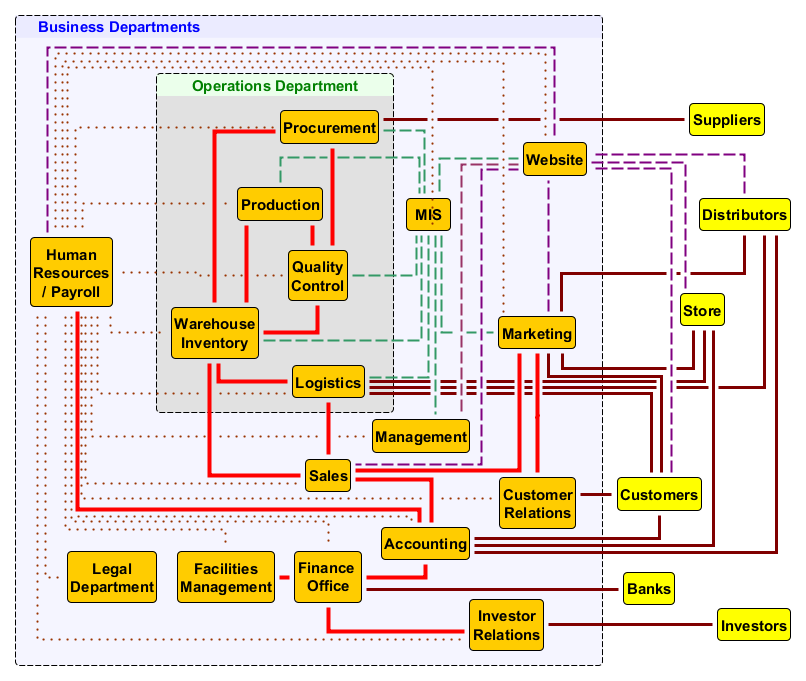
\includegraphics{images/businessdepts.png}
\caption{Interactions between business departments}
\end{figure}

Even with over 50 years of intensive development to reduce the complexity of doing business, new software tools and apps are still emerging at an astounding rate. The following sidebars attempt to classify common software systems found in medium to large size enterprises into 2 basic types of business systems.

\begin{itemize}
\item
  \textbf{Enterprise Resource Planning (ERP):} data systems that store and communicate operational data in a way facitates reporting and future planning.
\item
  \textbf{Enterprise Resource Management (ERM):} software systems that facilitate the monitor and manage interaction and the use of resources.
\end{itemize}

\BeginKnitrBlock{rmdextra}
\hypertarget{erp-software-systems}{%
\section*{ERP Software Systems}\label{erp-software-systems}}
\addcontentsline{toc}{section}{ERP Software Systems}

\begin{itemize}
\item
  \textbf{CONTENT MANAGEMENT SYSTEM (CMS):}

  \begin{itemize}
  \tightlist
  \item
    Collections of guides, rulebooks, forms, and procedure guidelines
  \item
    Blogs, newsletter, announcements
  \item
    Catalogues, price lists
  \item
    Documentation of intellectual property and licenses
  \end{itemize}
\item
  \textbf{PRODUCT INFORMATION MANAGEMENT (PIM):}

  \begin{itemize}
  \tightlist
  \item
    Manual, troubleshooting guides
  \item
    Parts list, equivalences
  \item
    Price lists and stock inventory
  \item
    Photos and promotional materials
  \end{itemize}
\item
  \textbf{Accounting Information System (AIS):}

  \begin{itemize}
  \tightlist
  \item
    Revenue: cash inflow (sales)
  \item
    Expenditure: cash outflow (payroll, equipment)
  \item
    Conversion: work-in-progress transactions (raw material, precursor inventory)
  \item
    Administrative: reporting (income statement, balance sheet, cash flows)
  \end{itemize}
\end{itemize}
\EndKnitrBlock{rmdextra}

\BeginKnitrBlock{rmdextra}
\hypertarget{erm-software-systems}{%
\section*{ERM Software systems}\label{erm-software-systems}}
\addcontentsline{toc}{section}{ERM Software systems}

\begin{itemize}
\item
  \textbf{B2B: Business-to-business software:} manages workflow with suppliers and partners

  \begin{itemize}
  \tightlist
  \item
    Directory of suppliers and products
  \item
    Social media confirmation of quality
  \end{itemize}
\item
  \textbf{B2C: Business-to-consumer software:} serve the needs of individual customers particularly in regards to customer history, order status, and billing information.

  \begin{itemize}
  \tightlist
  \item
    Online store
  \item
    Product manuals, product information
  \item
    Delivery tracking
  \end{itemize}
\item
  \textbf{Human Resources Management (HRM):}

  \begin{itemize}
  \tightlist
  \item
    Payroll, bonuses, raises
  \item
    Staff work experience, Performance appraisal, skill tests
  \item
    Flight risk, employee satisfaction
  \item
    Education, training
  \end{itemize}
\item
  \textbf{Marketing Automation Platform (MAP):}

  \begin{itemize}
  \tightlist
  \item
    CRM: Customer Relationship Management - purchase history, rewards, interests,
  \item
    MCP: Marketing Campaign Planning - Ad words, analytics, costs, contracts, effectiveness
  \end{itemize}
\end{itemize}
\EndKnitrBlock{rmdextra}

\hypertarget{essentials-of-business-quality-management}{%
\section{Essentials of Business Quality Management}\label{essentials-of-business-quality-management}}

Businesses are driven by an active communication chain that drives the business process. The effectiveness of teamwork and management depends on effective communication. However, the communication chain can be interrupted by bottlenecks in the flow of data, inconsistent or misleading reporting, and other communication breakdowns. Quality standards help ensure that processes related to production and quality control are subject to timely, data-driven management. In essence the ability of a business to fix a problem depends on the quality of communications that provide access to the description of the true nature and extend of the problem and knowledge of possible remedies.

\begin{figure}
\centering
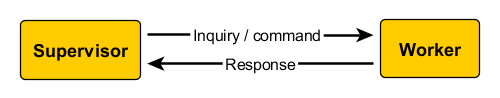
\includegraphics{images/communication.png}
\caption{Communication Chain}
\end{figure}

Meaningful communication requires a reciprocal interaction between the speaker and the listener. As shown in the following table, social norms and good ethicate depend on transmission of a message and an appropriate response. The communication chain is lost when messages in either direction are lost or misinterpreted. The growing use of social media with its emphasis on icons or one word responses has often been blamed for the reduction in quality of personal verbal and written skills. Interaction with customers and suppliers depends on clear and effective communication.

\begin{longtable}[]{@{}ll@{}}
\toprule
Initiation message & Response message\tabularnewline
\midrule
\endhead
Greeting & Acknowledgement\tabularnewline
Question & Response\tabularnewline
Proposal & Acceptance/Rejection\tabularnewline
Command & Action\tabularnewline
Accusation & Acceptance/Rebuttal\tabularnewline
\bottomrule
\end{longtable}

\hypertarget{iso9000iso9001}{%
\subsection{ISO9000/ISO9001}\label{iso9000iso9001}}

ISO 9000 was first published in 1987 by the International Organization for Standardization (ISO). The derivative quality standards help organizations address the needs of customers and while meeting relevant statutory and regulatory requirements.\citep{ISOweb} The ISO9001 standards provide guidance and tools for companies and organizations who want to ensure that their processes regularly deliver products and services that meet customer's requirements. It also defines the requirements for certification against these standards which are reviewed and revised every 5 years.\citep{ISO2015}

\begin{itemize}
\tightlist
\item
  \textbf{Point 1: Clear customer understanding} of the goods or services offered within a business contract.
\item
  \textbf{Point 2: Verification of intended results} to ensure that the terms of the business contract were met.
\item
  \textbf{Point 3: Prevention of undesired effects} that might cause delays or problems in the delivery of goods and services
\item
  \textbf{Point 4: Improve performance} based on the information gathered
\end{itemize}

\BeginKnitrBlock{rmddiscussion}
\textbf{An example of an ISO9001 compliant transaction}

Discuss what points of the ISO9001 standard is satisfied by the follow stages of a simple business transaction at a restuarant.

\begin{enumerate}
\def\labelenumi{\arabic{enumi}.}
\tightlist
\item
  The customer enters a restaurant and is given a menu with pictures of the food.
\item
  The waiter takes the order and repeats the order back to the customer for confirmation.
\item
  The waiter brings the food and doubles check that the order is complete.
\item
  The waiter comes back to check if everything is okay.
\item
  The cashier checks that all was well when the bill is paid.
\item
  The whole transaction is recorded and the receipt gives a website for feedback.
\item
  The customer's feedback on the website is analyzed for patterns of service that could be improved.
\end{enumerate}
\EndKnitrBlock{rmddiscussion}

\BeginKnitrBlock{rmdexercise}
\textbf{Exercise: ISO9001 and MacDonalds}

Worldwide MacDonald is a successful multinational enterprise run by staff most of which are under the age of 21 and yet it is a certified ISO9001 company. When a customer orders food at any MacDonald outlet in the world, the interaction between the customer and the counter staff is always the same.

\begin{itemize}
\tightlist
\item
  Create a swim lane workflow diagram to describe the information flow in the conversation between the customer, the counter staff, the kitchen staff, the accounting system, and the point-of-sale computer system.
\item
  Identify how the basic principles of ISO9001 principles for quality management are a ddressed by this basic operating procedure..
\end{itemize}
\EndKnitrBlock{rmdexercise}

\hypertarget{changes-to-business}{%
\section{Changes to Business}\label{changes-to-business}}

Businesses today have unprecedented opportunities to rapidly address issues that arise. Such advances in such fields as deep machine learning, Big Data analytics, Internet of Things, collective intelligence, online payment and social media are creating a reality that was only hinted at by the 1999 book \textbf{\emph{Business at the speed of thought.}} \citep{Gates1999} Businesses that were market leaders in the past, but failed to keep pace with the changes, suddenly find themselves bankrupt and replaced by new competitors. In 500BC, Heraclitus of Ephesus once penned the warning that ``Change is the only constant in life'' but he words ring true as an accurate description of today's business environment.

\hypertarget{open-organization}{%
\subsection{Open Organization}\label{open-organization}}

Since ISO9000 was first published in 1987, it has been revised and replaced by a long list of international standards that define and specify how various aspects of business, hardware, and software are to be implemented. Each new standard built on the principles already established and addresses the weaknesses of previous standards. \citep{ISO2015} While these developments help to ensure consistent service and quality, something else was needed to empower staff to collectively think and implement creative solutions to challenges. Jim Whitehurst at RedHat.com invested considerable effort to address this problem. He started with the realization that ``the best practices in creating open source software also translate well into managing an entire company.'' By embracing open source values and creating a new open standard for communities, he showed how leaders can successfully create ``a rebooted, redesigned, reinvented organization suitable for the decentralized, empowered, digital age.''\citep{Whitehurst2015} In creating the open organization, he and his colleagues have documented a shift that is changing in the way businesses are organized, managed and run.

\begin{longtable}[]{@{}ll@{}}
\toprule
\begin{minipage}[b]{0.47\columnwidth}\raggedright
Traditional values\strut
\end{minipage} & \begin{minipage}[b]{0.47\columnwidth}\raggedright
Post-Modern values\strut
\end{minipage}\tabularnewline
\midrule
\endhead
\begin{minipage}[t]{0.47\columnwidth}\raggedright
Loyality to the organizational hierachy\strut
\end{minipage} & \begin{minipage}[t]{0.47\columnwidth}\raggedright
Loyality to the mission, purpose and values of the company\strut
\end{minipage}\tabularnewline
\begin{minipage}[t]{0.47\columnwidth}\raggedright
Compliance\strut
\end{minipage} & \begin{minipage}[t]{0.47\columnwidth}\raggedright
Focus creativity to create solutions\strut
\end{minipage}\tabularnewline
\begin{minipage}[t]{0.47\columnwidth}\raggedright
Predictability\strut
\end{minipage} & \begin{minipage}[t]{0.47\columnwidth}\raggedright
Adaptability to change\strut
\end{minipage}\tabularnewline
\begin{minipage}[t]{0.47\columnwidth}\raggedright
Efficiency\strut
\end{minipage} & \begin{minipage}[t]{0.47\columnwidth}\raggedright
Effectiveness\strut
\end{minipage}\tabularnewline
\begin{minipage}[t]{0.47\columnwidth}\raggedright
Plan, Prescribe, Execute\strut
\end{minipage} & \begin{minipage}[t]{0.47\columnwidth}\raggedright
Envision, Prioritize, Implement, Adjust\strut
\end{minipage}\tabularnewline
\bottomrule
\end{longtable}

Successful, innovative organizations demonstrate the following core principles which form the basis for the core elements of open organizations. \citep{Whitehurst2019}

\begin{itemize}
\tightlist
\item
  The best ideas come from anywhere.
\item
  The best ideas should always win.
\item
  Contribution matters more than title.
\end{itemize}

\begin{figure}
\centering
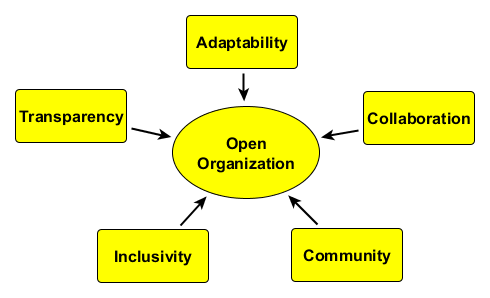
\includegraphics{images/openorg.png}
\caption{Core elements of open organizations}
\end{figure}

Although every open organization is unique, there is a common core of elements that characterize open organizations. Each core element is composed of a different dataset to be gathered, distributed, and combined in powerful and productive ways.

\begin{itemize}
\tightlist
\item
  \textbf{Transparency:} Workers have access to all pertinent information and willingly disclose and discuss their work. Workers can access and review the processes and arguments that lead to decisions and are free to comment and respond to them. Successes and failures are valued for the lessons they provide.
\item
  \textbf{Inclusivity:} Protocols and procedures are developed to encourage constructive discussion from diverse perspectives. Leaders actively seek to include voices not present in the dialog. Technology is used to ensure and encourage access to discussion forums.
\item
  \textbf{Adaptability:} Feedback mechanisms provide access for suggestions from members of the organizations and outside members.
\item
  \textbf{Collaboration:} The organization adheres to the principle that working together produces better results. Products of development are made available to other projects to use creatively.
\item
  \textbf{Community:} Shared values and principles that guide decision making are clear and obvious to members of the organization. All workers are encouraged and empowered to make meaningful contributions to the collaborative effort. Leaders mentor others and model shared values and principles.
\end{itemize}

As organizations embrace the core concepts of open organizations, they discover that openness is necessary for success and that attempts to pursue openness will lead to 3 possible outcomes: \citep{OOA2017}

\begin{itemize}
\item
  \textbf{Greater agility:} resulting from the synergy that arises when members share a common vision and work together toward common goals.
\item
  \textbf{Faster innovation:} because ideas from both inside and outside the organization receive more equitable consideration and rapid experimentation
\item
  \textbf{Increased engagement:} as members clearly see connections between their particular activities and an organization's overarching values, mission, and spirit.
\end{itemize}

\BeginKnitrBlock{rmdextra}
\hypertarget{working-as-a-developer-within-an-open-organization}{%
\section*{Working as a developer within an open organization}\label{working-as-a-developer-within-an-open-organization}}
\addcontentsline{toc}{section}{Working as a developer within an open organization}

Increasingly large IT development center like Google, Oracle and Apple are becoming open organizations to encourage and value innovation. Each worker in those companies is expected to do his/her part in contributing to the development effort. However, young IT staff have a very high rate of turn over as they are often foreign to working in environments that productively focus creativity to solve issues. This mismatch was the inspiration behind a recent blog concerning the five laws that development engineers should know. \citep{Short2017}

\begin{enumerate}
\def\labelenumi{\arabic{enumi}.}
\tightlist
\item
  \textbf{Forget the phrase `I do not know':} Treat every task as an opportunity to learn and dedicate the time needed to become an expert
\item
  \textbf{Read the manual! :} Documentation was written for a purpose. Do not waste colleague's time.
\item
  \textbf{Search before asking:} Do not contribute to the problems but contribute to the solution.
\item
  \textbf{Anything is possible:} Anything is possible in this space with proper time, coordination, and effort. Trust by verifying new ideas
\item
  \textbf{Acknowledge technical debt:} Technical debt is the result of decisions that made sense at the time someone made them but cause problems because they are not based on reality.
\end{enumerate}
\EndKnitrBlock{rmdextra}

\hypertarget{the-changing-nature-of-customers}{%
\subsection{The changing nature of customers}\label{the-changing-nature-of-customers}}

Advances in technology have changed both the ability to produce product and the nature of markets. The internet and social media have exposed individuals to a wider range of products and vendors. This creates new desires and expectations in customers and increased competition among business. At the same time, social changes are impacting markets, particularly as youth explore new careers, lifestyles, technologies, and life goals.

\BeginKnitrBlock{rmdextra}
\textbf{Changing indicators of success in Singapore}

The most common indicators of success mentioned in conversation with Singapore voters in 2000 was compare to the list compiled from conversations with Singaporen youth in 2018. \citep{SNYCYC2019}, \citep{Tan2019}

\begin{longtable}[]{@{}rll@{}}
\toprule
Level & Traditional success indicators & Goals of Singapore Youth\tabularnewline
\midrule
\endhead
1 & Career / Work & Emotional well being\tabularnewline
2 & Finance / Money & Personal learning / Skill development\tabularnewline
3 & Studies / Degrees & Family\tabularnewline
4 & Family & Finance / Money\tabularnewline
5 & House / Belongings & Spirituality\tabularnewline
\bottomrule
\end{longtable}

\textbf{Top 10 Life Goals Important to Singapore Youth}

\begin{longtable}[]{@{}lr@{}}
\toprule
Goals & Percent\tabularnewline
\midrule
\endhead
Home ownership & 70\%\tabularnewline
Strong family relationships & 70\%\tabularnewline
Learning / acquiring new skils & 62\%\tabularnewline
Successful career & 59\%\tabularnewline
Earn lots of money & 46\%\tabularnewline
Help less fortunate & 41\%\tabularnewline
Contribute to society & 40\%\tabularnewline
Get married & 36\%\tabularnewline
Have children & 35\%\tabularnewline
Good religious life & 31\%\tabularnewline
\bottomrule
\end{longtable}
\EndKnitrBlock{rmdextra}

Today's businesses need to be as versatile and diverse as the customers and markets they serve. In the past, only businesses with a large customer base were about to benefit from economies of scale. However, online services have made it possible for businesses to support both mass distribution to millions of consumers while at the same time of catering to the diverse needs of individual customers that number in the millions.

\BeginKnitrBlock{rmddiscussion}
\textbf{Discussion: Impact of changes in life goals on business}

\begin{enumerate}
\def\labelenumi{\arabic{enumi}.}
\item
  How do you think changes in life goals of youth will impact the market place?
\item
  Based on these changes, which products would be expected to have the greatest increases or decreases in demand in the next 10 or 20 years?
\item
  What aspirations of Thai youth have changed in the last 10 years?
\item
  What impact will these changes have on the Thai economy?
\end{enumerate}
\EndKnitrBlock{rmddiscussion}

In addition, social media provide a forum for expressing opinions without being held accountable for the view expressed. Generally, the rewards for being liked help to regulate the web but increasing courts are given the power to litigate on defamation cases where rumors have caused damage. Nonetheless, social media continue to have an impact on Brand and Product Marketing,particularly in the following ways.

\begin{enumerate}
\def\labelenumi{\arabic{enumi}.}
\tightlist
\item
  Word-of-mouth referrals from trusted acquaintances are powerful endorsements and attractions.
\item
  Customer testimonials are often decisive in purchasing decisions.
\item
  Community discussion of the products being developed increases trust in the company.
\item
  False testimonies are a problem: fakes entries attempt to oversell a product or provide complaints in an attempt to destroy the company.
\item
  Online searches and discussions are becoming the primary source of information for most.
\end{enumerate}

\BeginKnitrBlock{rmddiscussion}
Given the changes in the nature of the online market, discuss how the following approaches help to target the population to focus on those who are most likely to purchase. For each of these approaches, identify the nature of a particular market for which it would be more effective than the others.

\begin{enumerate}
\def\labelenumi{\arabic{enumi}.}
\tightlist
\item
  Search engine ads based on topics being searched
\item
  Social media ads based on shared views and ideas
\item
  Personal profiling to drive the user experience at a website based on specific interests and preferences expressed
\end{enumerate}
\EndKnitrBlock{rmddiscussion}

\hypertarget{changing-nature-of-business}{%
\subsection{Changing nature of business}\label{changing-nature-of-business}}

It is clear that the retail companies in rapid growth are those who are able to upgrade the services of the traditional storefront into a more convenient, efficient and user-friendly setting that compliments the services available online. Banks have moved their services online and to ATM to increase the convenience of handling money while lowering operating costs. Online companies like Amazon have teamed up with traditional shopping chains like Target to allows customers the opportunity to compare, touch and feel products before purchasing them either in the shop or online. Online orders can be delivered to shops to reduce shipping costs. Amazon has even integrated such high tech features as AI, face recognition and sensor to change the user shopping experience.\citep{Amazon2016} Technology play a critical role in all of these developments.

\BeginKnitrBlock{rmddiscussion}
\hypertarget{new-generation-7-11-seven-eleven}{%
\section*{New generation 7-11 (Seven Eleven)}\label{new-generation-7-11-seven-eleven}}
\addcontentsline{toc}{section}{New generation 7-11 (Seven Eleven)}

View this news clip about a new Seven Eleven outlet that opened in Pattaya with a new look that is in keeping with the era of Thailand 4.0. The store is full of sensors, monitors and systems to create a modern, futuristic, efficient shopping and eating environment complete with innovations to improve energy-saving and user convenience. Watch the video \citep{Suriywong2018} and list the number of ways computers have been used to change the user experience.
\EndKnitrBlock{rmddiscussion}

\hypertarget{online-commerce}{%
\section{Online Commerce}\label{online-commerce}}

In 2019, it is estimated that over 56\% of the world's population has access to the internet. There are 26.6 billion devices and 4.39 billion people are connected to the internet. It is estimated that 3.48 billion social media users. Facebook alone has well over 2.36 billion users each month. Google answers 63,000 searches per second. This is creating unprecented levels of opportunity for marketing to huge markets world-wide. In the following graph, the number of users grows linearly while their revenues grow expotentally. \citep{Statista2019}

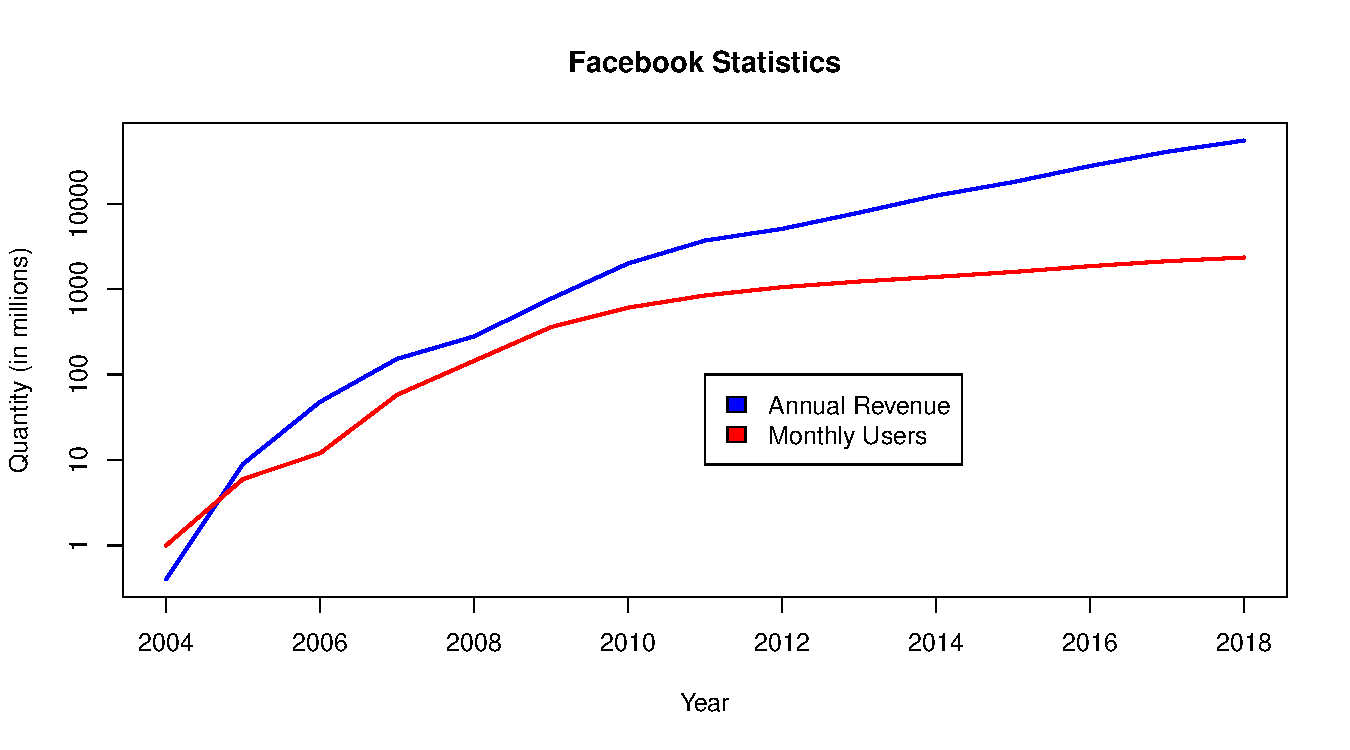
\includegraphics{bookdown-demo_files/figure-latex/unnamed-chunk-4-1.pdf}

\BeginKnitrBlock{rmddiscussion}
\textbf{The mobile phone market}
Review the statistics of the performance of leading mobile phone producers since 1994 {[}TNW2019{]} and discuss the following:

\begin{itemize}
\tightlist
\item
  What factors contributed to the fall of market leaders?
\item
  How will President Trump's technology embargo on China effect this market?
\item
  Is there room for new competitors in this market?
\end{itemize}
\EndKnitrBlock{rmddiscussion}

\hypertarget{growth-of-the-internet-and-e-commerce}{%
\subsection{Growth of the Internet and e-commerce}\label{growth-of-the-internet-and-e-commerce}}

As the following graph shows, the types of devices used to access the internet have also changed in the past decade.

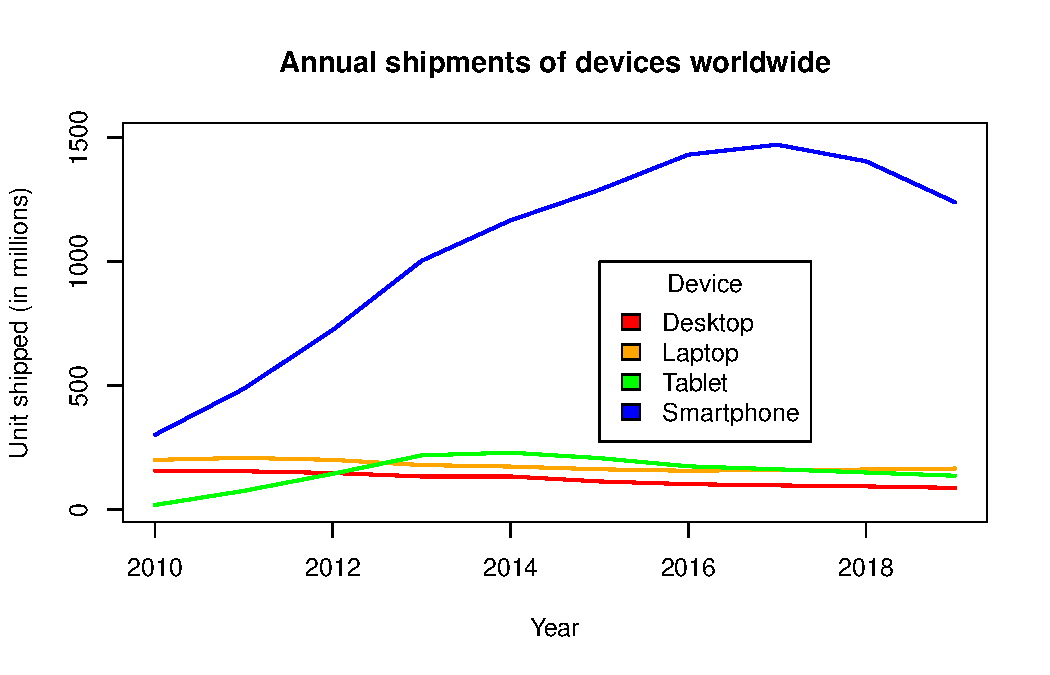
\includegraphics{bookdown-demo_files/figure-latex/unnamed-chunk-5-1.pdf}

The trend has been to using mobile devices for shopping, and surfing for possibilities. There appears to be some resistance to using mobile devices to order online.

\begin{longtable}[]{@{}rccc@{}}
\toprule
& Computer & Tablet & Smartphone\tabularnewline
\midrule
\endhead
E-commerce traffic & 53.9\% & 12.4\% & 33.7\%\tabularnewline
Volume of Retail sales & 76.9\% & 12.4\% & 10.7\%\tabularnewline
\bottomrule
\end{longtable}

With the development of the world wide web in the 1990s, online commerce has been gaining advantage over corresponding brick and mortar firms, especially for the following reasons:

\begin{enumerate}
\def\labelenumi{\arabic{enumi}.}
\tightlist
\item
  The customer has access to more information to make better purchasing decisions
\item
  The customer can shop 24x7
\item
  The customer can track the progress of order fulfillment.
\item
  Customers can find and provide feedback verified through social media.
\item
  The functions of e-commerce can be purchased and updated to keep development costs low and to maximize economies of scale
\end{enumerate}

However, the elderly are more resistant to adopt online shopping, but there is growing acceptance.

\textbf{Adoption of online shopping by age of internet user}

\begin{longtable}[]{@{}llllll@{}}
\toprule
Frequency & 18-29 & 30-39 & 40-49 & 50-64 & \textgreater{}65\tabularnewline
\midrule
\endhead
Once per week & 35\% & 37\% & 23\% & 17\% & 11\%\tabularnewline
Once per month & 41\% & 35\% & 35\% & 38\% & 31\%\tabularnewline
Once per year & 24\% & 28\% & 42\% & 45\% & 50\%\tabularnewline
Never & 0\% & 0\% & 0\% & 0\% & 8\%\tabularnewline
\bottomrule
\end{longtable}

\begin{figure}
\centering
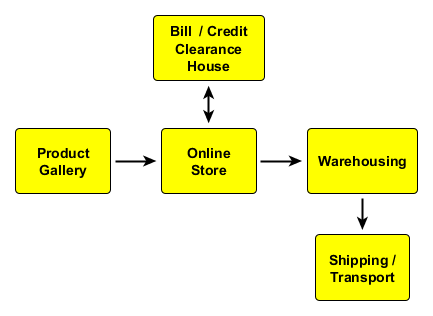
\includegraphics{images/ecommercefunctions.png}
\caption{Business Functions of E-Commerce}
\end{figure}

\hypertarget{the-e-shopping-customer-experience}{%
\subsection{The e-shopping customer experience}\label{the-e-shopping-customer-experience}}

As shown by the table below, The process of shopping for goods online has many similarities to shopping at traditional brick and mortar shops. These similarities have contributed to rapid growth in online purchases which in 2018 totaled \$2,489 trillion worldwide. This represents about 8.8\% of all sales worldwide. \citep{Saleh2019}

\begin{longtable}[]{@{}lll@{}}
\toprule
\begin{minipage}[b]{0.15\columnwidth}\raggedright
Stage\strut
\end{minipage} & \begin{minipage}[b]{0.38\columnwidth}\raggedright
Brick and Mortar\strut
\end{minipage} & \begin{minipage}[b]{0.38\columnwidth}\raggedright
Electronic world\strut
\end{minipage}\tabularnewline
\midrule
\endhead
\begin{minipage}[t]{0.15\columnwidth}\raggedright
Customer finds the store.\strut
\end{minipage} & \begin{minipage}[t]{0.38\columnwidth}\raggedright
Ads and billboards\strut
\end{minipage} & \begin{minipage}[t]{0.38\columnwidth}\raggedright
Google and Facebook Ads; Referrals from blogs\strut
\end{minipage}\tabularnewline
\begin{minipage}[t]{0.15\columnwidth}\raggedright
Customer shops for items of interest\strut
\end{minipage} & \begin{minipage}[t]{0.38\columnwidth}\raggedright
Window shopping\strut
\end{minipage} & \begin{minipage}[t]{0.38\columnwidth}\raggedright
Search the website\strut
\end{minipage}\tabularnewline
\begin{minipage}[t]{0.15\columnwidth}\raggedright
Customer searches for information on the products\strut
\end{minipage} & \begin{minipage}[t]{0.38\columnwidth}\raggedright
Check packaging and sales staff\strut
\end{minipage} & \begin{minipage}[t]{0.38\columnwidth}\raggedright
Internet searches and social media recommendations\strut
\end{minipage}\tabularnewline
\begin{minipage}[t]{0.15\columnwidth}\raggedright
Customer chooses items for purchase\strut
\end{minipage} & \begin{minipage}[t]{0.38\columnwidth}\raggedright
Places them in a cart or shopping basket\strut
\end{minipage} & \begin{minipage}[t]{0.38\columnwidth}\raggedright
Virtual transfer of items to an electronic shopping cart\strut
\end{minipage}\tabularnewline
\begin{minipage}[t]{0.15\columnwidth}\raggedright
Customer checkouts the selected items for purchase\strut
\end{minipage} & \begin{minipage}[t]{0.38\columnwidth}\raggedright
The customer takes the shopping cart to the check out counter\strut
\end{minipage} & \begin{minipage}[t]{0.38\columnwidth}\raggedright
The virtual cart is checked out creating a preliminary bill complete with shipping information\strut
\end{minipage}\tabularnewline
\begin{minipage}[t]{0.15\columnwidth}\raggedright
The financial institution identifies and authenticates the payer\strut
\end{minipage} & \begin{minipage}[t]{0.38\columnwidth}\raggedright
The customer swipes a credit card or ATM card\strut
\end{minipage} & \begin{minipage}[t]{0.38\columnwidth}\raggedright
The customer logs into to e-banking, e-payment or credit card services\strut
\end{minipage}\tabularnewline
\begin{minipage}[t]{0.15\columnwidth}\raggedright
The customer transfers funds to the vendor.\strut
\end{minipage} & \begin{minipage}[t]{0.38\columnwidth}\raggedright
The customer signs the electronic receipt or pays cash\strut
\end{minipage} & \begin{minipage}[t]{0.38\columnwidth}\raggedright
The customer verifies and authorizes payment\strut
\end{minipage}\tabularnewline
\begin{minipage}[t]{0.15\columnwidth}\raggedright
The financial institution send payment verification.\strut
\end{minipage} & \begin{minipage}[t]{0.38\columnwidth}\raggedright
ATM or Credit card service authenticates the transaction or the cashier\strut
\end{minipage} & \begin{minipage}[t]{0.38\columnwidth}\raggedright
The financial institution sends a secure memo to the e-store that payment was made.\strut
\end{minipage}\tabularnewline
\begin{minipage}[t]{0.15\columnwidth}\raggedright
The vendor sends a pick-list order to the fulfillment center.\strut
\end{minipage} & \begin{minipage}[t]{0.38\columnwidth}\raggedright
The storekeeper faxes the order to the warehouse\strut
\end{minipage} & \begin{minipage}[t]{0.38\columnwidth}\raggedright
The fulfillment center is notified of the order and its payment and picks the items\strut
\end{minipage}\tabularnewline
\begin{minipage}[t]{0.15\columnwidth}\raggedright
The fulfillment center sends the goods to the shipper.\strut
\end{minipage} & \begin{minipage}[t]{0.38\columnwidth}\raggedright
The items are boxed and set aside for pickup\strut
\end{minipage} & \begin{minipage}[t]{0.38\columnwidth}\raggedright
The items are boxed and sent to the shipper.\strut
\end{minipage}\tabularnewline
\begin{minipage}[t]{0.15\columnwidth}\raggedright
The fulfillment center updates the order status.\strut
\end{minipage} & \begin{minipage}[t]{0.38\columnwidth}\raggedright
The customer is called to pick up his order.\strut
\end{minipage} & \begin{minipage}[t]{0.38\columnwidth}\raggedright
The online system is updated and the customer can track its location.\strut
\end{minipage}\tabularnewline
\begin{minipage}[t]{0.15\columnwidth}\raggedright
The shipper delivers the goods.\strut
\end{minipage} & \begin{minipage}[t]{0.38\columnwidth}\raggedright
The counter staff check the delivery items and turns them over to the customer.\strut
\end{minipage} & \begin{minipage}[t]{0.38\columnwidth}\raggedright
The shipper delivers the goods.\strut
\end{minipage}\tabularnewline
\begin{minipage}[t]{0.15\columnwidth}\raggedright
The customer takes possession of the goods.\strut
\end{minipage} & \begin{minipage}[t]{0.38\columnwidth}\raggedright
The customer picks up the bags and leaves\strut
\end{minipage} & \begin{minipage}[t]{0.38\columnwidth}\raggedright
The customer signs for the goods and the tracking system is updated.\strut
\end{minipage}\tabularnewline
\bottomrule
\end{longtable}

\BeginKnitrBlock{rmddiscussion}
\hypertarget{hybrid-businesses}{%
\section{Hybrid businesses}\label{hybrid-businesses}}

Online shopping giant Amazon has recently merged with Target a traditional department store chain. Explain why this merger is a good idea and what benefits the customer gains from it.
\EndKnitrBlock{rmddiscussion}

\hypertarget{business-software-models}{%
\chapter{BUSINESS SOFTWARE MODELS}\label{business-software-models}}

This chapter will explore some common approaches to model the network of interactions that occur for business processes. These models not only help to provide deeper understanding of the nature of a business process but can facilating the development of systems to collect and analyze the data associated with the process.

\hypertarget{business-process-model-bpm}{%
\section{Business Process Model (BPM)}\label{business-process-model-bpm}}

There are many good reasons for using BPMN to model business processes. \citep{Camunda2018a}

\begin{itemize}
\tightlist
\item
  \textbf{Recognized Standard:} BPMN is owned by an institution and is supported by many software products. Third party BPMN editors are available in the form of desktop apps like yEd \citep{YED2018} or online services like Camunda. \citep{Camunda2018b}
\item
  \textbf{Simplicity:} BPMN is based on a system of graphic symbols that easy to learn.
\item
  \textbf{Power of expression:} BPMN reduces descriptions of complex process work flows to a graphic model that is easy to grasp.
\item
  \textbf{Implementation in IT:} BPMN was developed to support technical implementation of processes (``Process Automation''). The more important IT becomes in a company, the more helpful BPMN can be, especially when process changes can be accomplished by a simple change of line.
\end{itemize}

\hypertarget{a-simple-example}{%
\subsection{A simple example}\label{a-simple-example}}

A BPMN model described a process from the beginning (a light or green circle) to the end (a dark red circle). Blocks of tasks leading to key events are specified in sequential order.

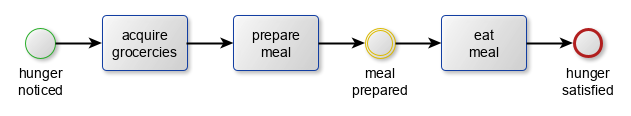
\includegraphics[width=1\linewidth]{images/simpleBPM}

\hypertarget{notation}{%
\subsection{Notation}\label{notation}}

Naming conventions help to improve the readability of the process:

\begin{itemize}
\item
  \textbf{Tasks:}

  \begin{itemize}
  \tightlist
  \item
    shown as a rounded rectangle
  \item
    described as a \texttt{{[}verb{]}\ +\ {[}object{]}}
  \item
    \emph{Acquire groceries} is better than \emph{first take care of shopping for groceries}
  \end{itemize}
\item
  \textbf{Events:}

  \begin{itemize}
  \tightlist
  \item
    description of milestones and achievements
  \item
    described as something that has already happened
  \item
    \emph{hunger noticed} is better \emph{when I begin to feel hungry}
  \end{itemize}
\end{itemize}

\hypertarget{symbols}{%
\subsection{Symbols}\label{symbols}}

BMP Software provide a pallette of objects to describe various aspects of a process.

\begin{figure}
\centering
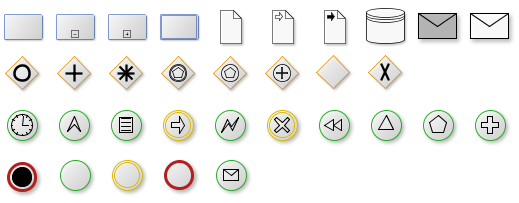
\includegraphics{images/yedpalette.png}
\caption{yEd BPMN Symbol Palette}
\end{figure}

\begin{figure}
\centering

\includegraphics{images/cawemopalette.png}
\caption{Cawemo BPMN Symbol Palette}
\end{figure}

\begin{longtable}[]{@{}cl@{}}
\toprule
Symbol & Description\tabularnewline
\midrule
\endhead

\includegraphics{images/start-event.png} & Start Event: Start of the process chain\tabularnewline

\includegraphics{images/end-event.png} & End Event: The end of the process chain\tabularnewline

\includegraphics{images/event-message-catch.png} & Event Message Catch: wait for a message event\tabularnewline

\includegraphics{images/event-message-throw.png} & Event Message Throw: sending a message event\tabularnewline
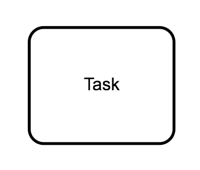
\includegraphics{images/task.png} & Task: Work to be done\tabularnewline

\includegraphics{images/xor-gateway.png} & XOR Gateway: choice of a action stream\tabularnewline

\includegraphics{images/parallel-gateway.png} & Parallel Gateway: initiate simulataneous action stream\tabularnewline
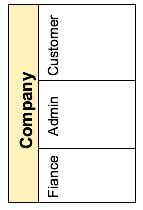
\includegraphics{images/swimlanes.png} & Swim lanes: separate the process by roles or actors\tabularnewline
\bottomrule
\end{longtable}

\hypertarget{sample-business-process-models}{%
\subsection{Sample Business Process Models}\label{sample-business-process-models}}

\begin{figure}
\centering
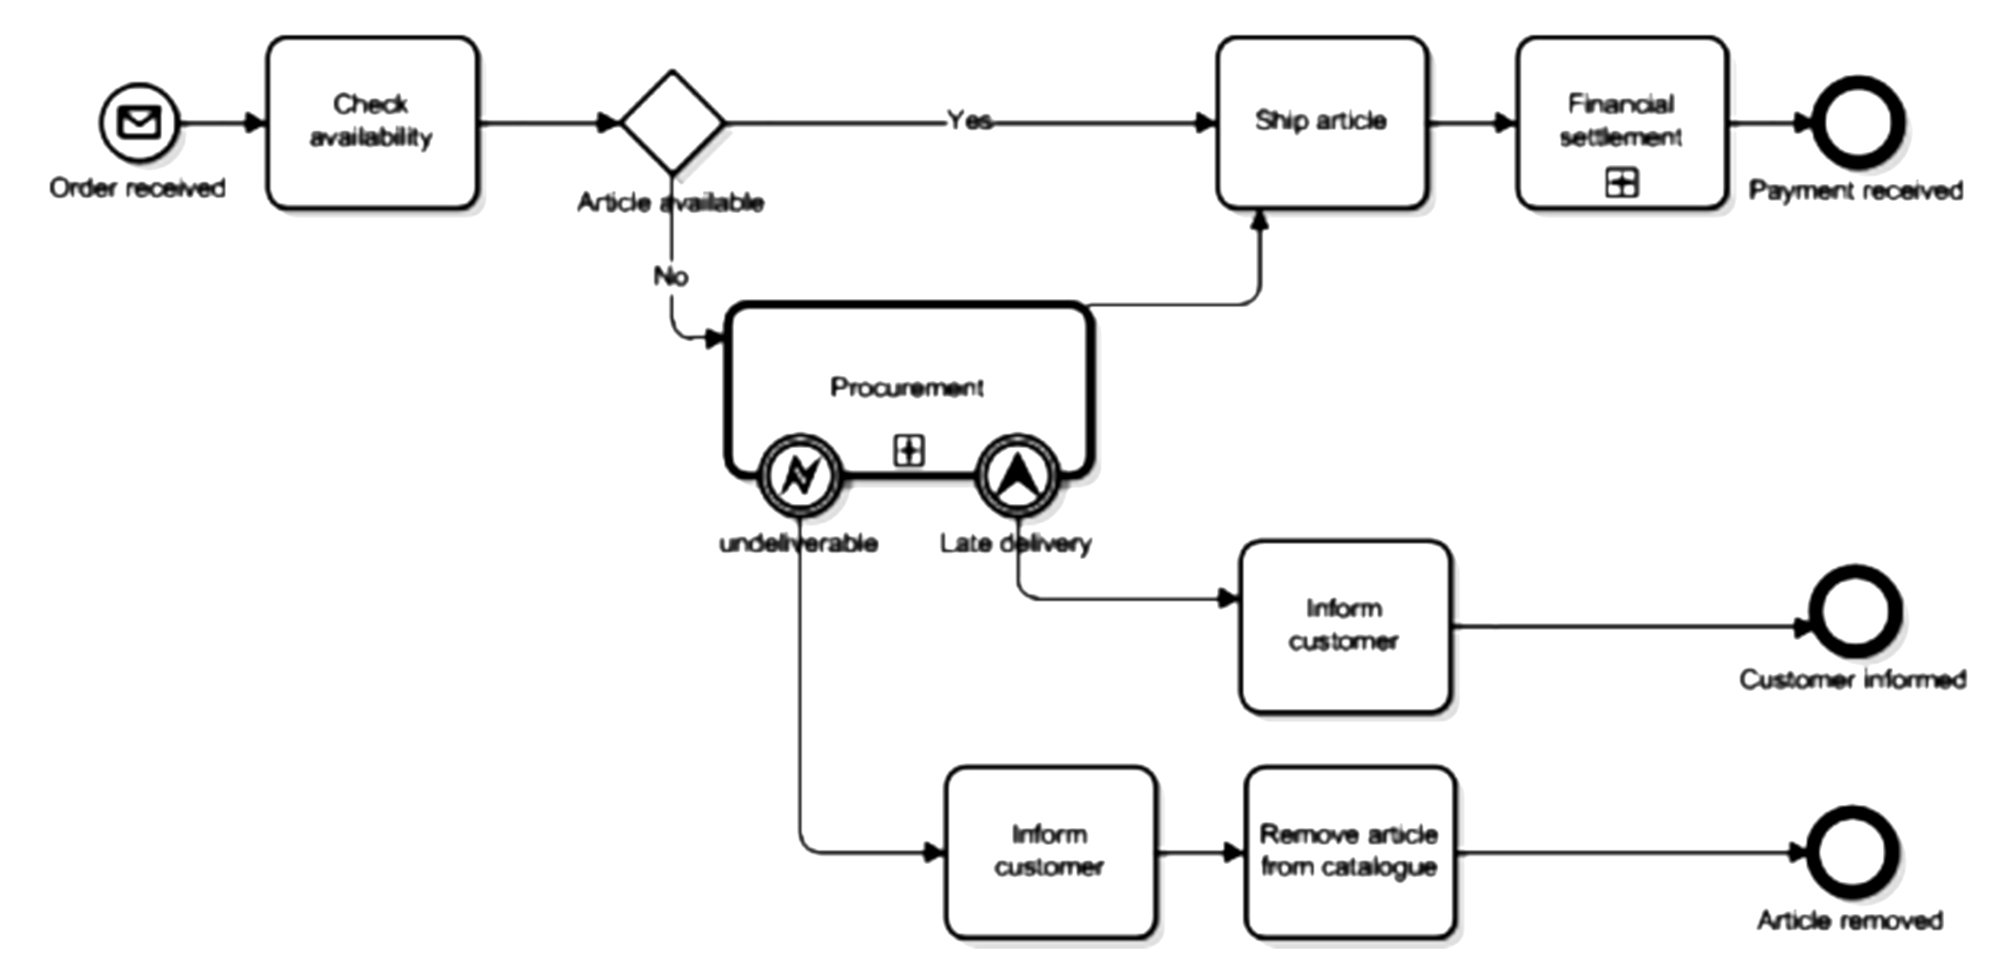
\includegraphics{images/orderfulfillment.png}
\caption{Order Fulfillment Processing}
\end{figure}

\begin{figure}
\centering
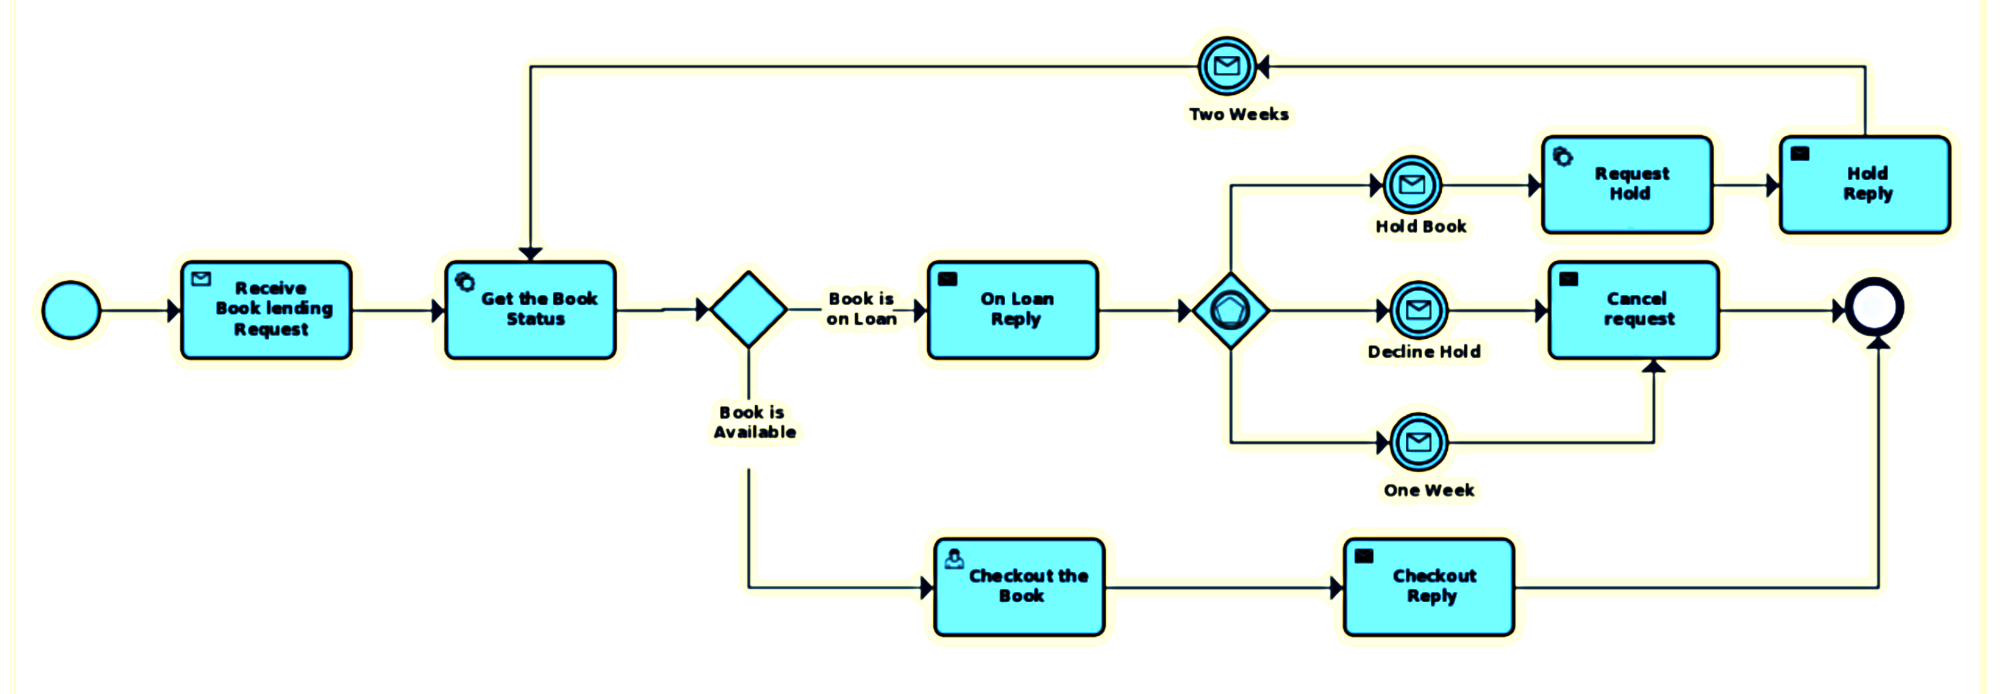
\includegraphics{images/bookckout.png}
\caption{Book Checkout at the Library}
\end{figure}

\begin{figure}
\centering
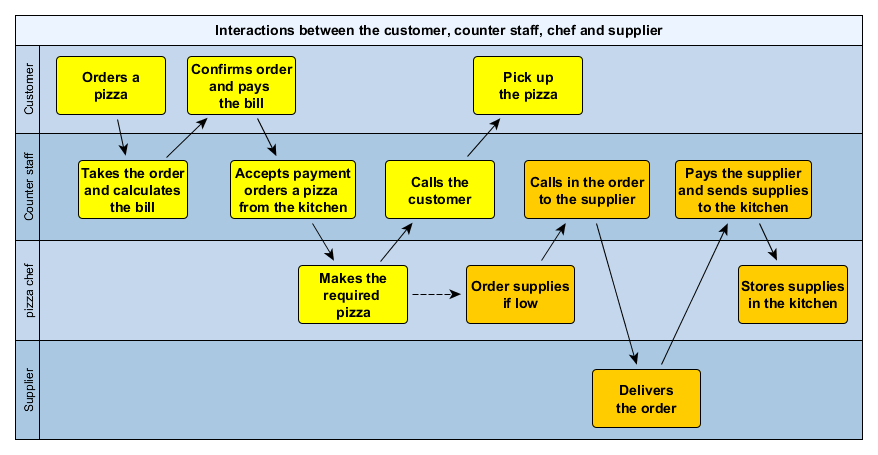
\includegraphics{images/pizza.png}
\caption{Pizza ordering}
\end{figure}

\begin{figure}
\centering
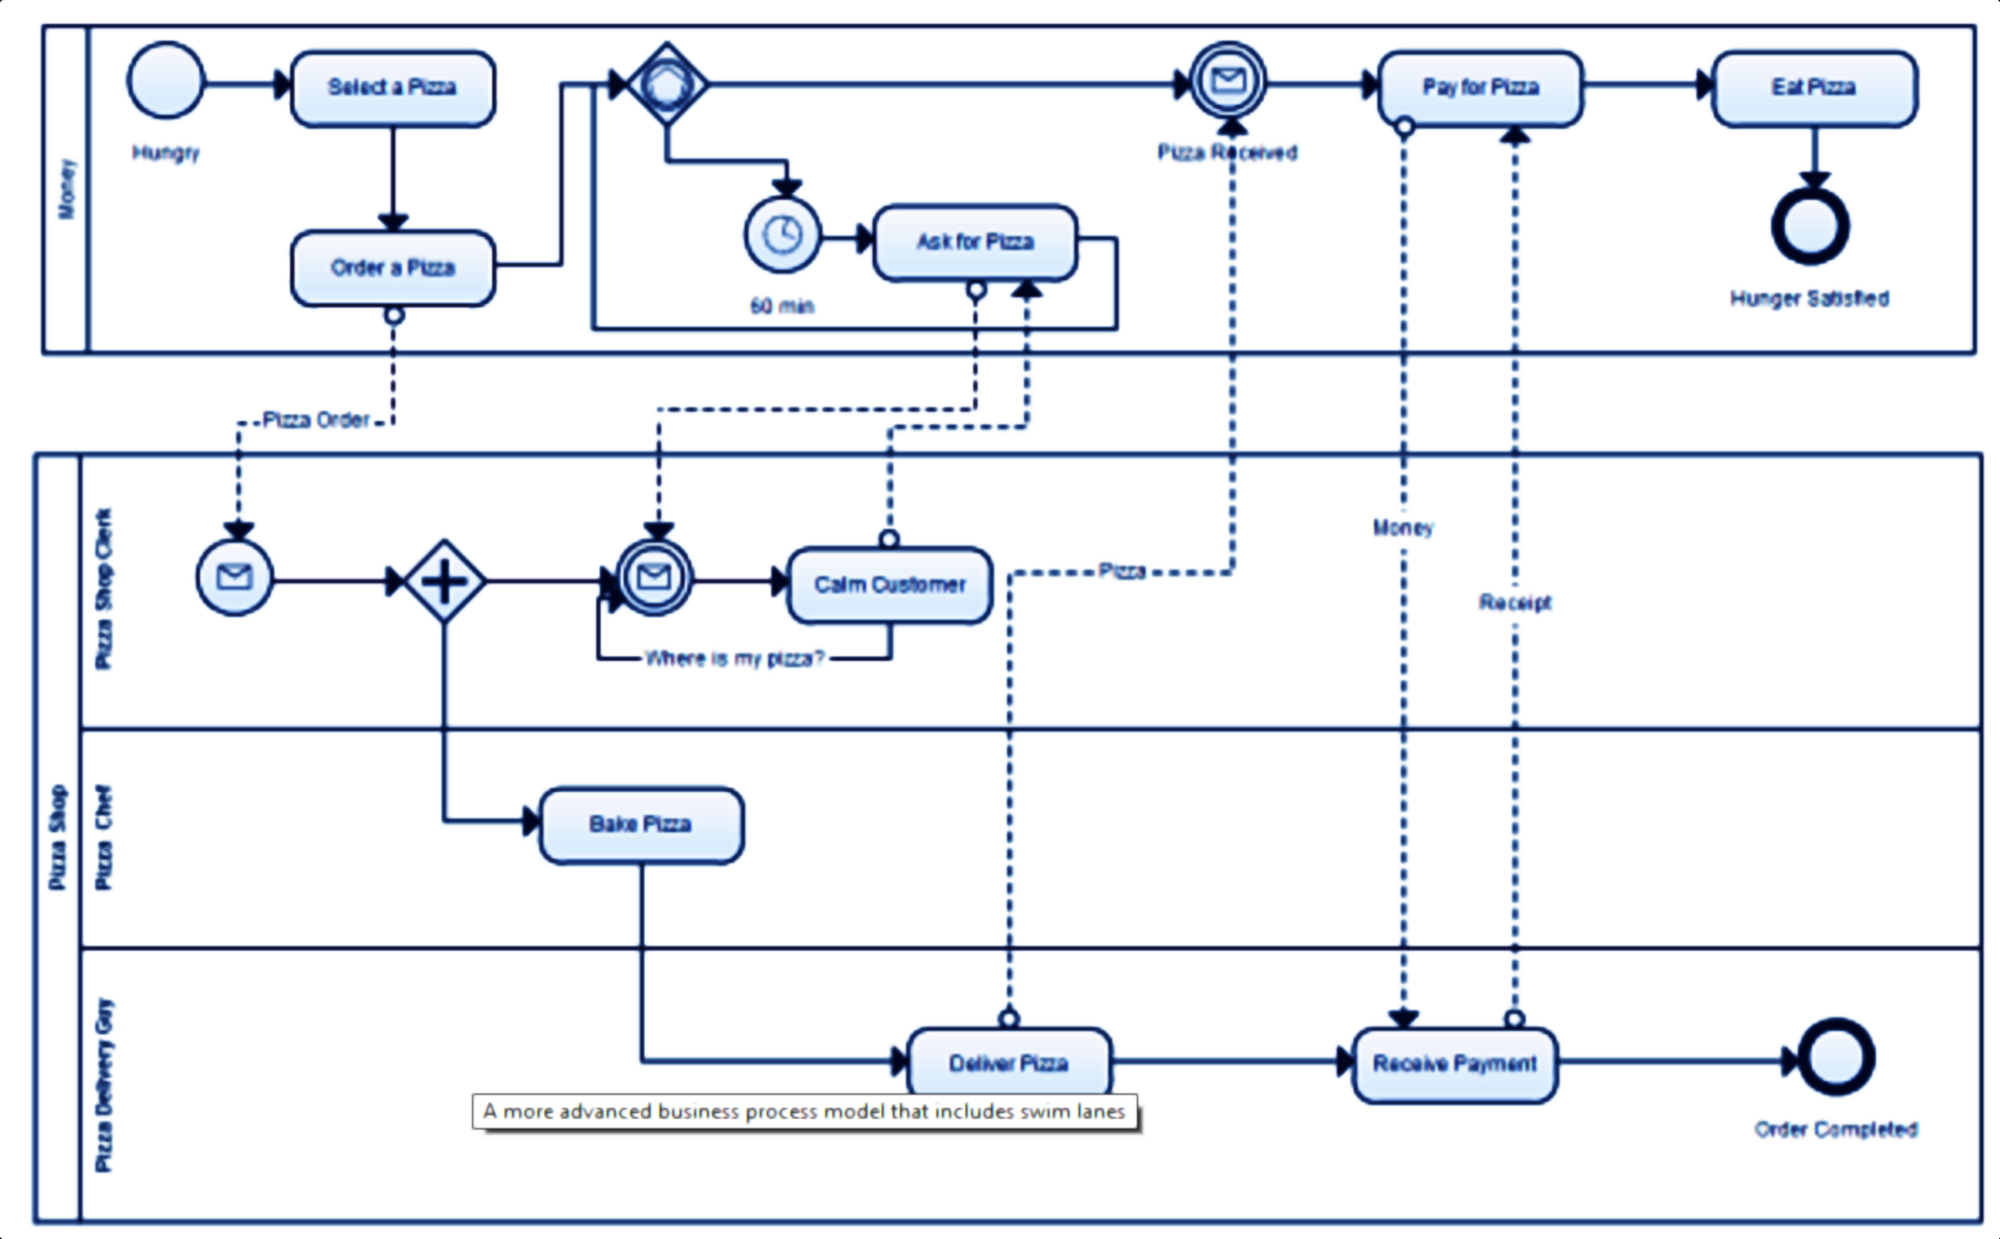
\includegraphics{images/pizza2.png}
\caption{Pizza shop}
\end{figure}

\BeginKnitrBlock{rmdexercise}
\textbf{Correcting a bug in process flow}

Identify and correct the flaw in this process so that
the grass can be weeded, cut and watered in that order but only as required.
\EndKnitrBlock{rmdexercise}

\begin{figure}
\centering
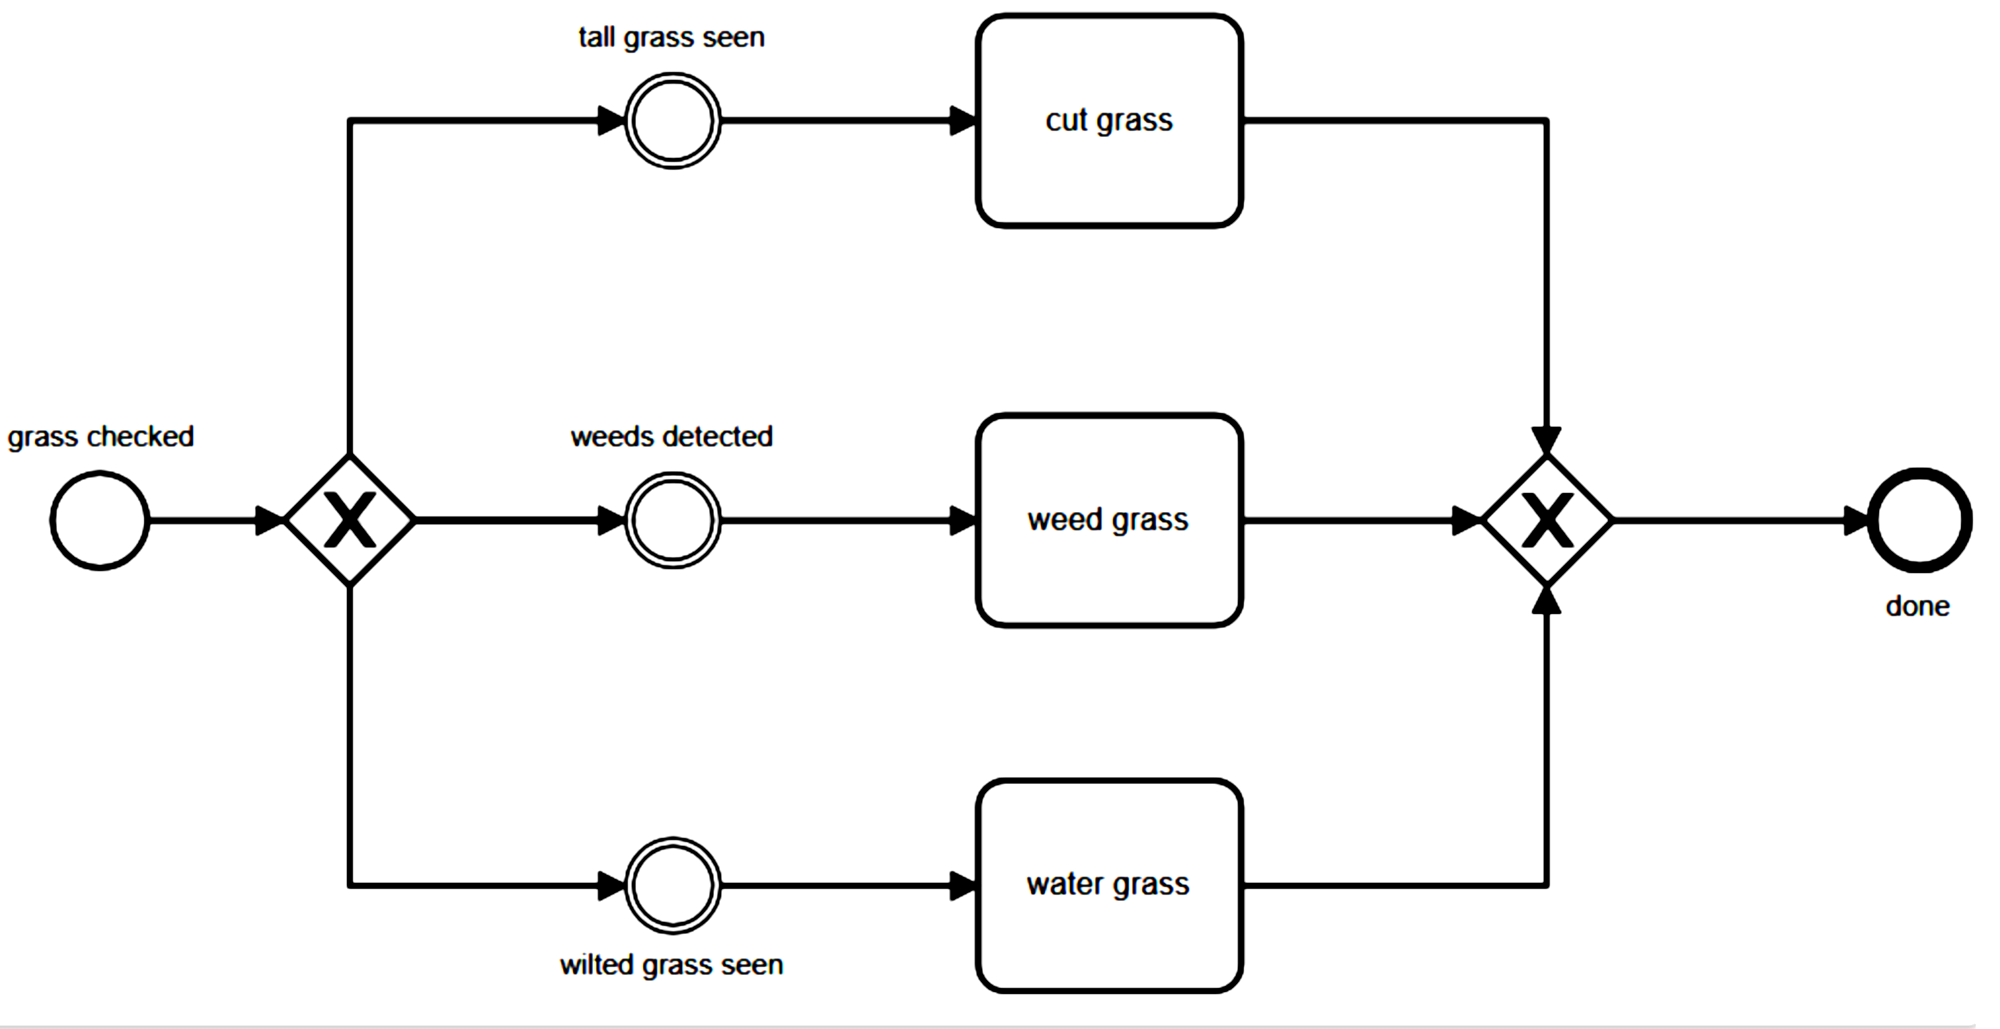
\includegraphics{images/cutgrass.png}
\caption{Cutting the grass}
\end{figure}

\hypertarget{bpmn-model-simulation}{%
\section{BPMN Model Simulation}\label{bpmn-model-simulation}}

BP Model sumulators allow process designers to test their model. The general approach is to use a task generator that creates and processes tasks at rates equal to the measured performance in the work place. Data is collected to measure the rate of utilization and work flow at all stages of the model in order to identify issues like bottlenecks and irregularities in the work loads of individual employees. Simulation test are usually conducted in 3 phases:

\begin{longtable}[]{@{}lll@{}}
\toprule
\begin{minipage}[b]{0.22\columnwidth}\raggedright
Stage\strut
\end{minipage} & \begin{minipage}[b]{0.41\columnwidth}\raggedright
Description\strut
\end{minipage} & \begin{minipage}[b]{0.28\columnwidth}\raggedright
Purpose\strut
\end{minipage}\tabularnewline
\midrule
\endhead
\begin{minipage}[t]{0.22\columnwidth}\raggedright
Modeling\strut
\end{minipage} & \begin{minipage}[t]{0.41\columnwidth}\raggedright
Simple visual model of the business process\strut
\end{minipage} & \begin{minipage}[t]{0.28\columnwidth}\raggedright
Specify the individual roles and the business logic of the process\strut
\end{minipage}\tabularnewline
\begin{minipage}[t]{0.22\columnwidth}\raggedright
Simulation\strut
\end{minipage} & \begin{minipage}[t]{0.41\columnwidth}\raggedright
Run task generation and execution according to measured performance\strut
\end{minipage} & \begin{minipage}[t]{0.28\columnwidth}\raggedright
Test the model based on work place rates of service\strut
\end{minipage}\tabularnewline
\begin{minipage}[t]{0.22\columnwidth}\raggedright
Analysis\strut
\end{minipage} & \begin{minipage}[t]{0.41\columnwidth}\raggedright
Creates a dashboard of performance indicators\strut
\end{minipage} & \begin{minipage}[t]{0.28\columnwidth}\raggedright
Verifies process design; Identifies opportunities for process improvement; Helps to maximize employee utilization; Provides for performance-based estimates of cost\strut
\end{minipage}\tabularnewline
\bottomrule
\end{longtable}

Online services such as \url{http://www.bpsimulator.com} provide a useful means for testing a process design through the display of the model, test results dashboard and performance indicators for each stage of the process. The design is actually a translation of a BPMN model into a Event-driven Process Chain (EPC). However, additional key details are required to quantify the capacity and number of resources available. These details are saved in the attributes for each node as shown in the next section.

\hypertarget{bp-simulator-model-components}{%
\subsection{BP Simulator Model Components}\label{bp-simulator-model-components}}

The following table is adapted from the online help of BPSimulation. \citep{BPSSimulator2018}

\begin{longtable}[]{@{}ll@{}}
\toprule
\begin{minipage}[b]{0.46\columnwidth}\raggedright
Object Description\strut
\end{minipage} & \begin{minipage}[b]{0.48\columnwidth}\raggedright
Example\strut
\end{minipage}\tabularnewline
\midrule
\endhead
\begin{minipage}[t]{0.46\columnwidth}\raggedright
\textbf{Function:} Set of targeted actions to be performed by one or more executors in one role\strut
\end{minipage} & \begin{minipage}[t]{0.48\columnwidth}\raggedright

\includegraphics{images/function.png} \newline      Repair of water supply; Acceptance payment; Sending a message\strut
\end{minipage}\tabularnewline
\begin{minipage}[t]{0.46\columnwidth}\raggedright
\textbf{Execute:} Position or role of those responsible for the execution of the function\strut
\end{minipage} & \begin{minipage}[t]{0.48\columnwidth}\raggedright
Motorman; Board member\strut
\end{minipage}\tabularnewline
\begin{minipage}[t]{0.46\columnwidth}\raggedright
\textbf{Resource:} Service or tools needed to perform the function\strut
\end{minipage} & \begin{minipage}[t]{0.48\columnwidth}\raggedright

\includegraphics{images/resource.png} \newline Machine; tool; Software\strut
\end{minipage}\tabularnewline
\begin{minipage}[t]{0.46\columnwidth}\raggedright
\textbf{Tasks Generator:} Generator global tasks of the business process of a certain type with a certain interval for the simulation purposes\strut
\end{minipage} & \begin{minipage}[t]{0.48\columnwidth}\raggedright

\includegraphics{images/generator.png} \newline Client request for a loan; Received customer complaint\strut
\end{minipage}\tabularnewline
\begin{minipage}[t]{0.46\columnwidth}\raggedright
\textbf{Checkpoint:} Auxiliary element for monitoring the process parameters at different stages its execution and control of tasks flow\strut
\end{minipage} & \begin{minipage}[t]{0.48\columnwidth}\raggedright

\includegraphics{images/checkpoint.png} \newline Completing the approval stage; Completion of the process because of inconsistencies detected\strut
\end{minipage}\tabularnewline
\begin{minipage}[t]{0.46\columnwidth}\raggedright
\textbf{Event:} Cause or an intangible result of a function\strut
\end{minipage} & \begin{minipage}[t]{0.48\columnwidth}\raggedright

\includegraphics{images/event.png} \newline  Client's visit; An error was detected\strut
\end{minipage}\tabularnewline
\begin{minipage}[t]{0.46\columnwidth}\raggedright
\textbf{Regulate:} Regulate document directly related to the order, conditions or results of the function\strut
\end{minipage} & \begin{minipage}[t]{0.48\columnwidth}\raggedright

\includegraphics{images/regulate.png} \newline  Manuals; Federal Law\strut
\end{minipage}\tabularnewline
\begin{minipage}[t]{0.46\columnwidth}\raggedright
\textbf{Input:} Material or information necessary to perform the function\strut
\end{minipage} & \begin{minipage}[t]{0.48\columnwidth}\raggedright

\includegraphics{images/input.png} \newline Form; Statement\strut
\end{minipage}\tabularnewline
\begin{minipage}[t]{0.46\columnwidth}\raggedright
\textbf{Output:} Material or information generated or acquired additional properties as a result of the function\strut
\end{minipage} & \begin{minipage}[t]{0.48\columnwidth}\raggedright

\includegraphics{images/output.png} \newline  Part; Conclusion\strut
\end{minipage}\tabularnewline
\begin{minipage}[t]{0.46\columnwidth}\raggedright
\textbf{Procedure:} Set of performance features for a particular purpose\strut
\end{minipage} & \begin{minipage}[t]{0.48\columnwidth}\raggedright

\includegraphics{images/procedure.png} \newline Applications processing; Approval of documentation\strut
\end{minipage}\tabularnewline
\begin{minipage}[t]{0.46\columnwidth}\raggedright
\textbf{Comment:} Auxiliary element model for clarifications or comments\strut
\end{minipage} & \begin{minipage}[t]{0.48\columnwidth}\raggedright
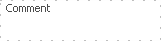
\includegraphics{images/comment.png} \newline     Temporary condition; Proposed improvements\strut
\end{minipage}\tabularnewline
\bottomrule
\end{longtable}

\hypertarget{linking-objects-together}{%
\subsection{Linking objects together}\label{linking-objects-together}}

All objects in the model should be at least one link to another object. To create a link between objects, you must first double-click on the object - the source of links, and then click on the object - the recipient, link will be created with an arrow on the side of the second object. Link means a direct impact or relationship of one object from another. Not all objects can be linked to each other. The group of objects: Tasks Generator, Function, Events, Procedure and Check Point can be suppliers (predecessors) or consumers (followers) of each other. Other objects only as the impact on function, as shown below the diagram:

\begin{figure}
\centering
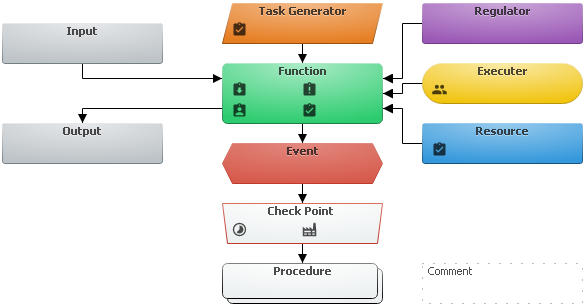
\includegraphics{images/exmodeling5.png}
\caption{Linking of Objects}
\end{figure}

With this extra data it is possible to simulate a day at work. The statistics collected help to pinpoint bottlenecks and limiting resources. The system provides a dashboard to summarize the results.

\begin{figure}
\centering
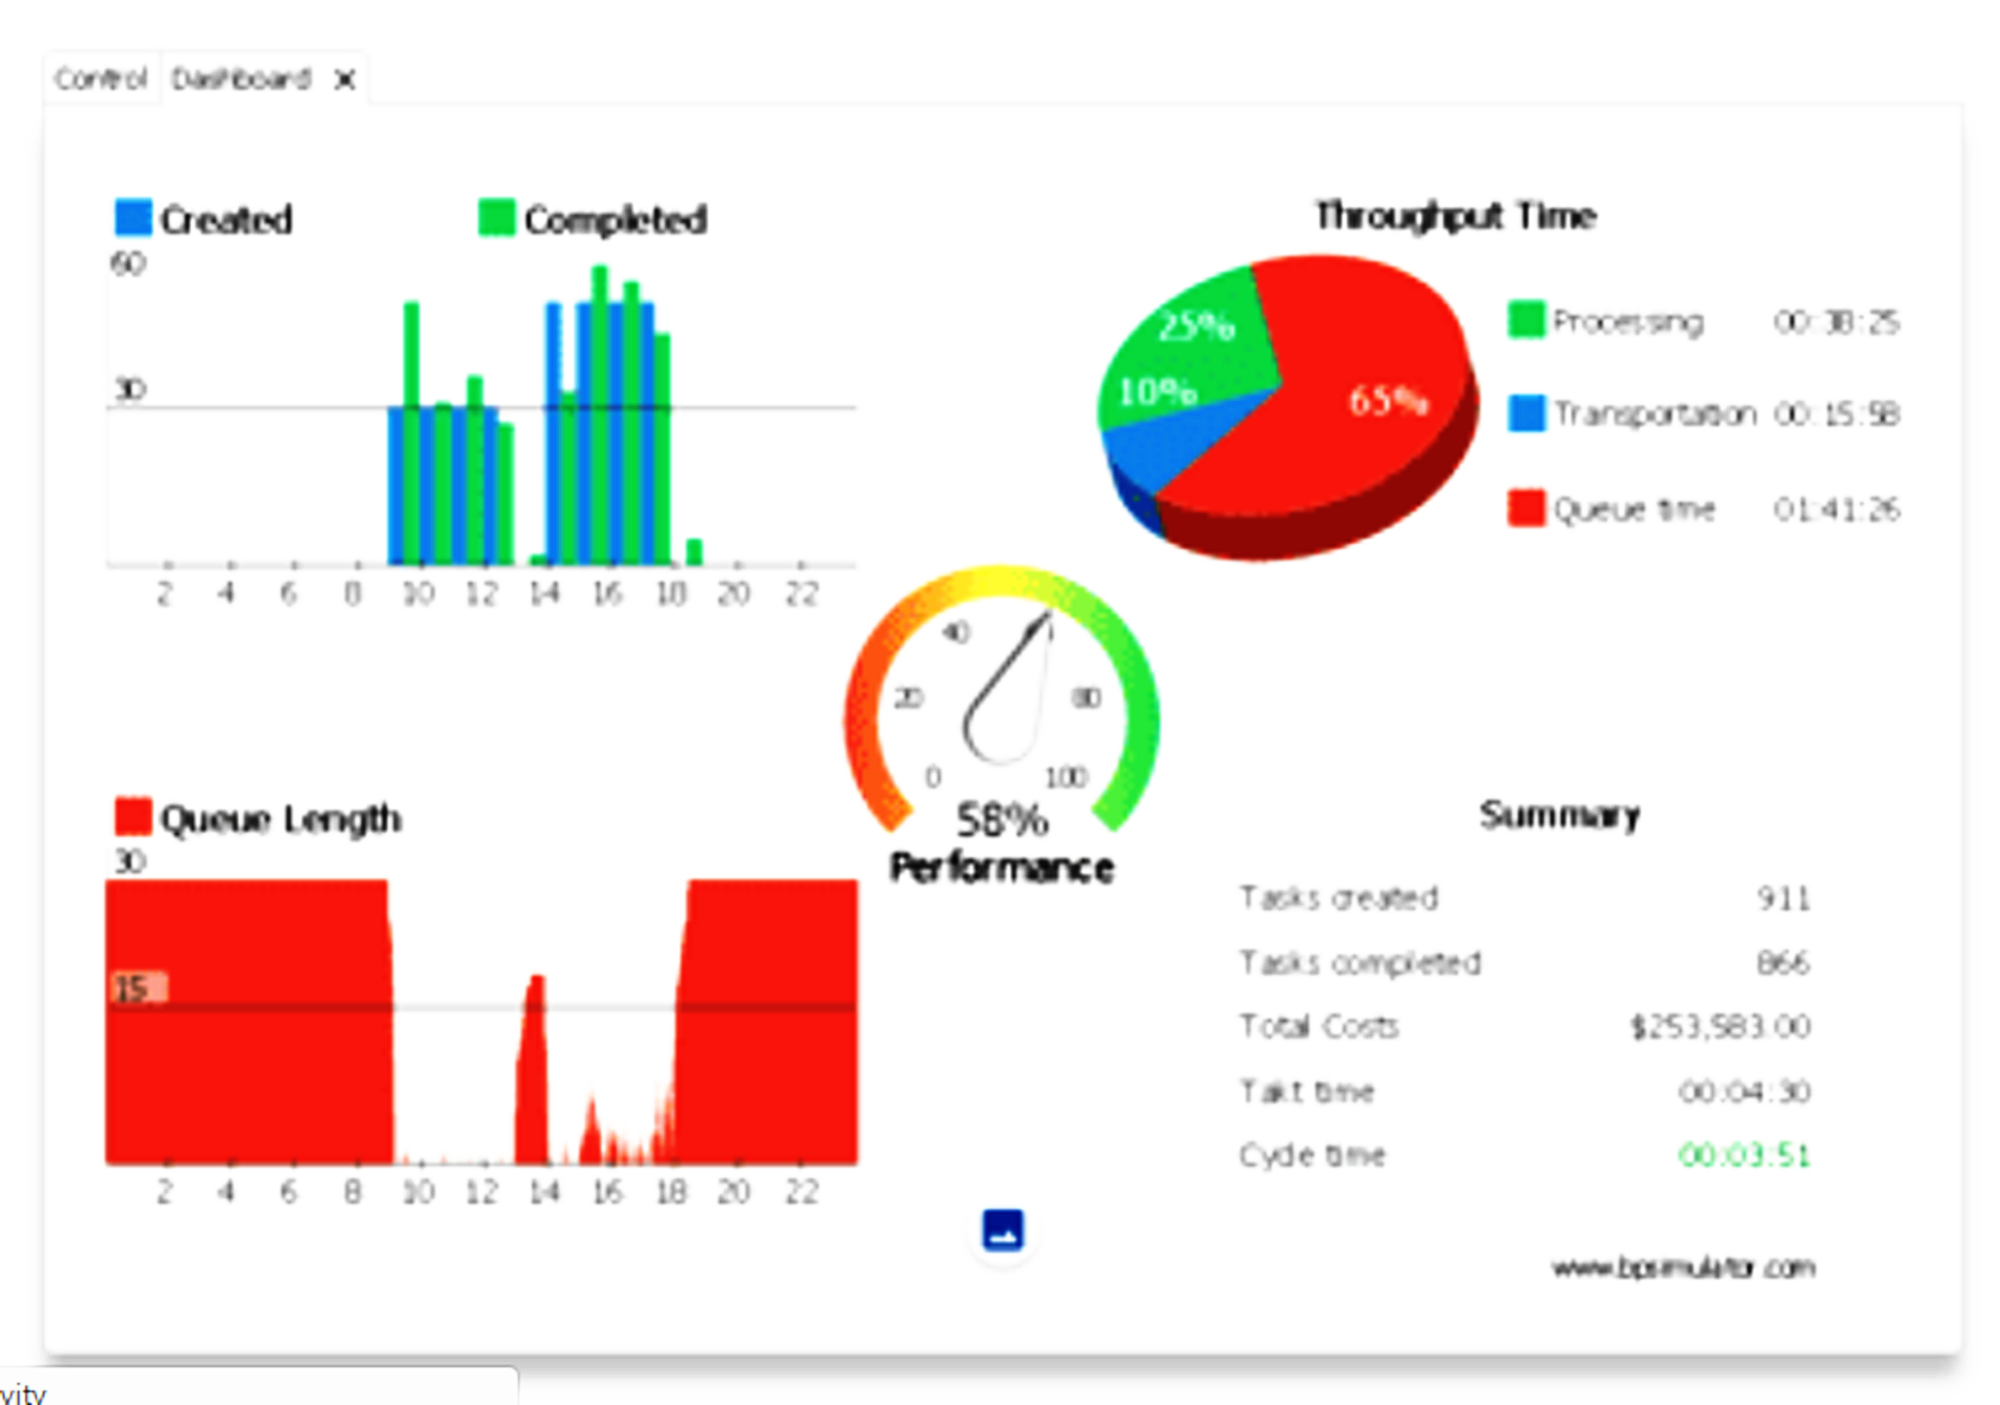
\includegraphics{images/bpsim2.png}
\caption{Dashboard of Test Results}
\end{figure}

The model uses generators to simulate the volume of the demand for needs. Data comes from the functions and key check points of the model that monitor the workflow that passes these nodes. The executor nodes determine the capacity of the system. Performance is varied by changing the number of individuals in the role of executors.

\begin{figure}
\centering
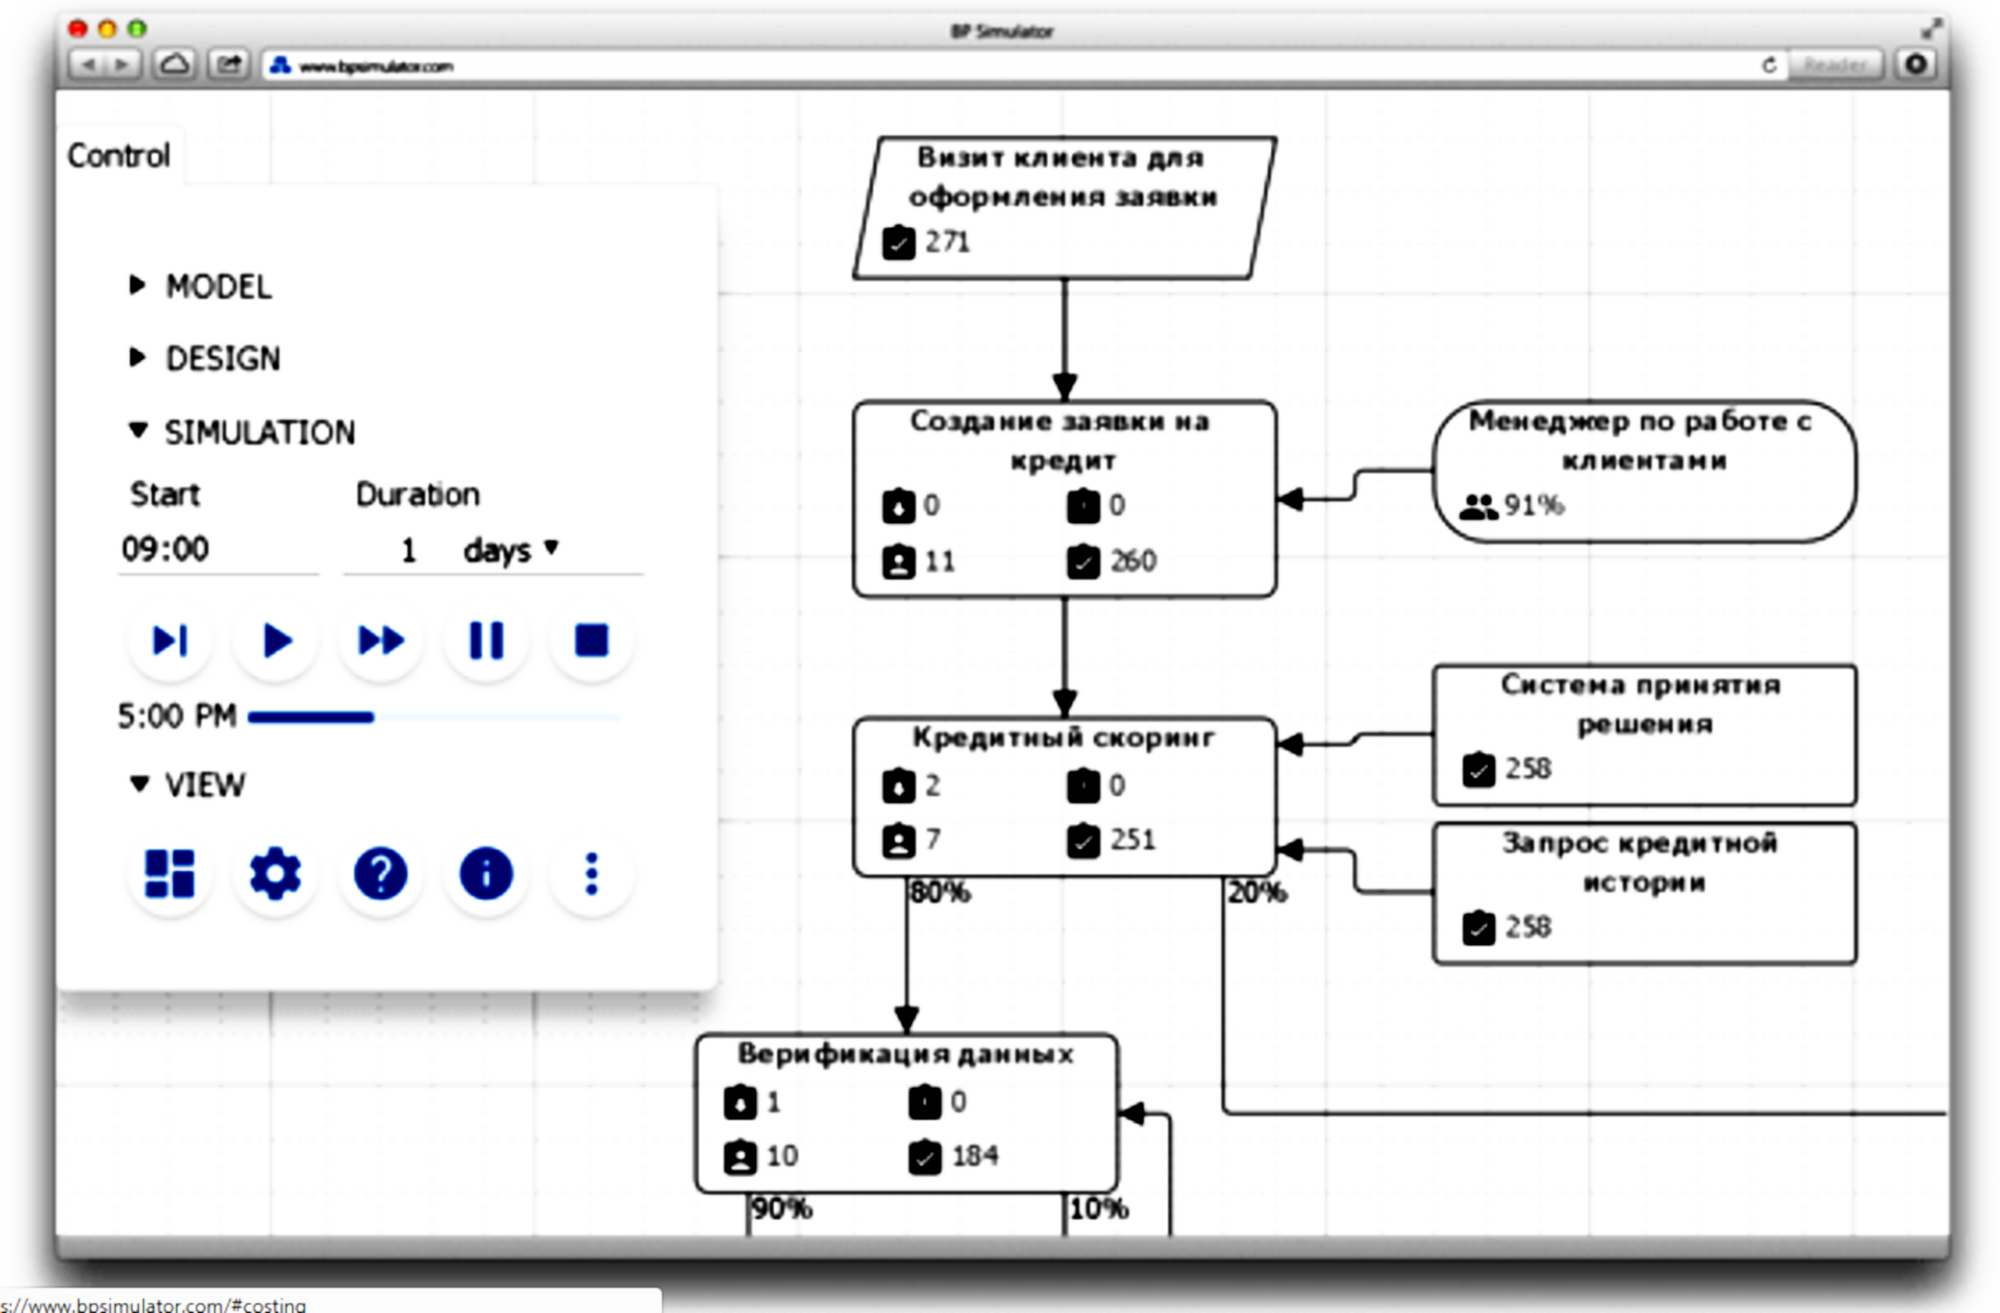
\includegraphics{images/bpsim3.png}
\caption{Performance indicators}
\end{figure}

\hypertarget{an-example-a-petrol-station}{%
\subsection{An example: A Petrol Station**}\label{an-example-a-petrol-station}}

Starting with the BPMN of a simple model of the processes behind getting gas at the petrol station.

\begin{figure}
\centering
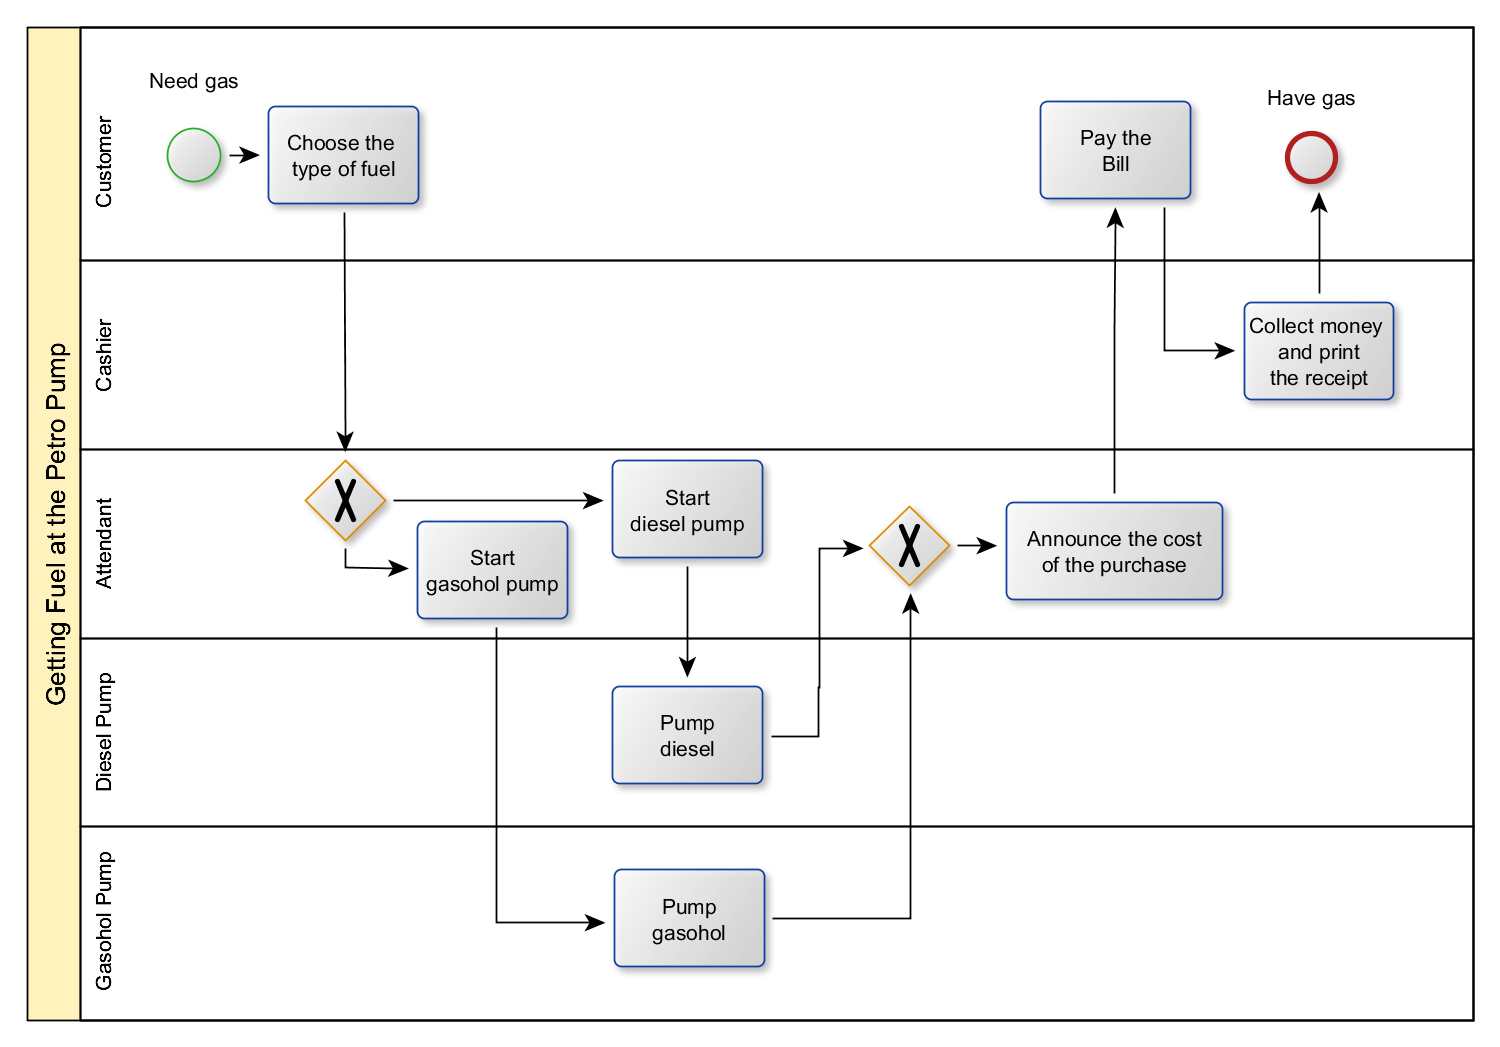
\includegraphics{images/gaspump.png}
\caption{The Gas Station}
\end{figure}

results in a simulated model within the BPSimulator.

\begin{figure}
\centering
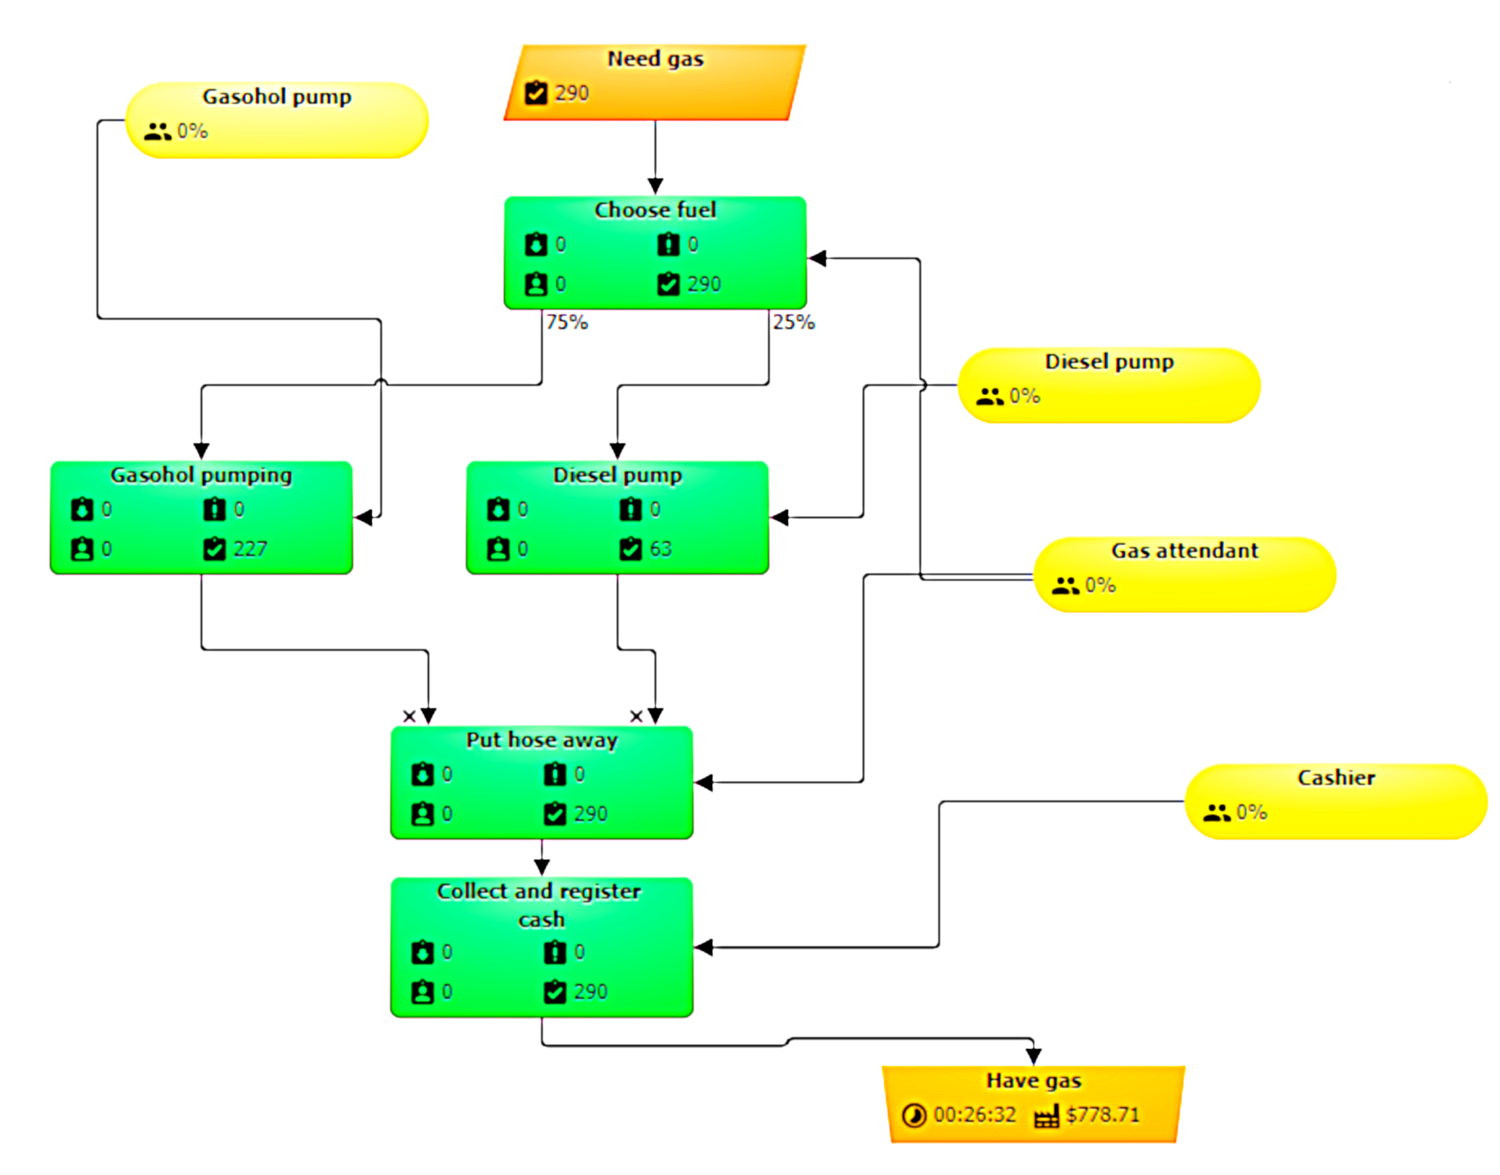
\includegraphics{images/gaspumpsim.png}
\caption{Getting Fuel Simulatation}
\end{figure}

The simulation was run in the scenario of only have one cashier, one attendant, one gasohol pump, one diesel pump and 290 customers who arrive.

\begin{longtable}[]{@{}llll@{}}
\toprule
Starting & Ending & Number & Hourly Rate\tabularnewline
\midrule
\endhead
6:00 & 8:59 & 90 & 30\tabularnewline
9:00 & 14:59 & 90 & 15\tabularnewline
15:00 & 18:59 & 90 & 25\tabularnewline
19:00 & 20:00 & 20 & 10\tabularnewline
\bottomrule
\end{longtable}

As shown in the dashboard, the average queue is 16 min.

\begin{figure}
\centering
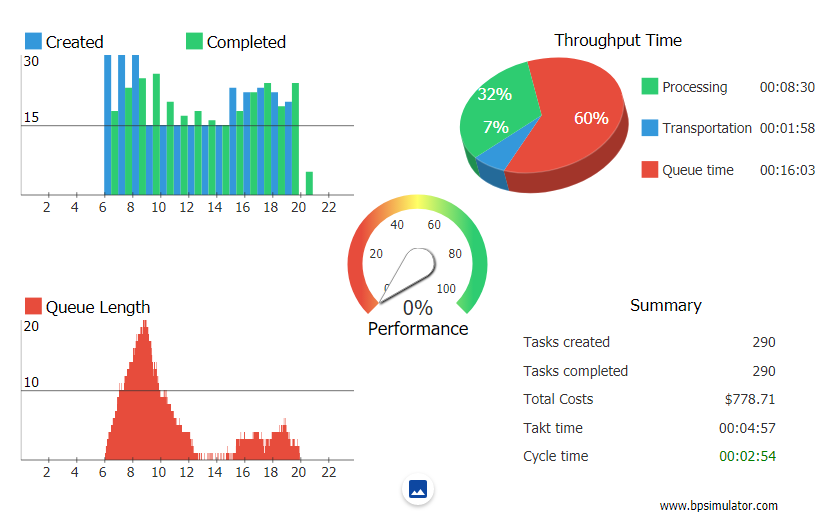
\includegraphics{images/gaspumpdash.png}
\caption{Dashboard for Getting Fuel}
\end{figure}

\BeginKnitrBlock{rmdexercise}
\textbf{Exercise: Improving performance of a petrol station}

Using the sample model of a petrol station, determine a proper mix of men and machines that will reduce the queue time to less than 2 mins at the minimum cost.
\EndKnitrBlock{rmdexercise}

\hypertarget{enterprise-resource-erp}{%
\section{Enterprise Resource (ERP)}\label{enterprise-resource-erp}}

The purpose of Enterprise Resource Planning (ERP) is to harness business data in a way that allows integrated management of core business processes. This business-management software is typically designed as a suite of integrated applications which collect, store, manage, and interpret data from a wide range of business activities. By managing the critical information of all business processes, ERP provides opportunities to support data-driven management decisions is such areas as cash flow, resources usage, inventory of raw materials, and the status of business commitments such as project milestones, orders fulfilment, purchase order payments, and staff compensation. The system facilitates the sharing of data across divisions of the business, such as manufacturing, purchasing, sales, accounting, and human resources.

\hypertarget{building-blocks}{%
\subsection{Building Blocks}\label{building-blocks}}

\begin{figure}
\centering
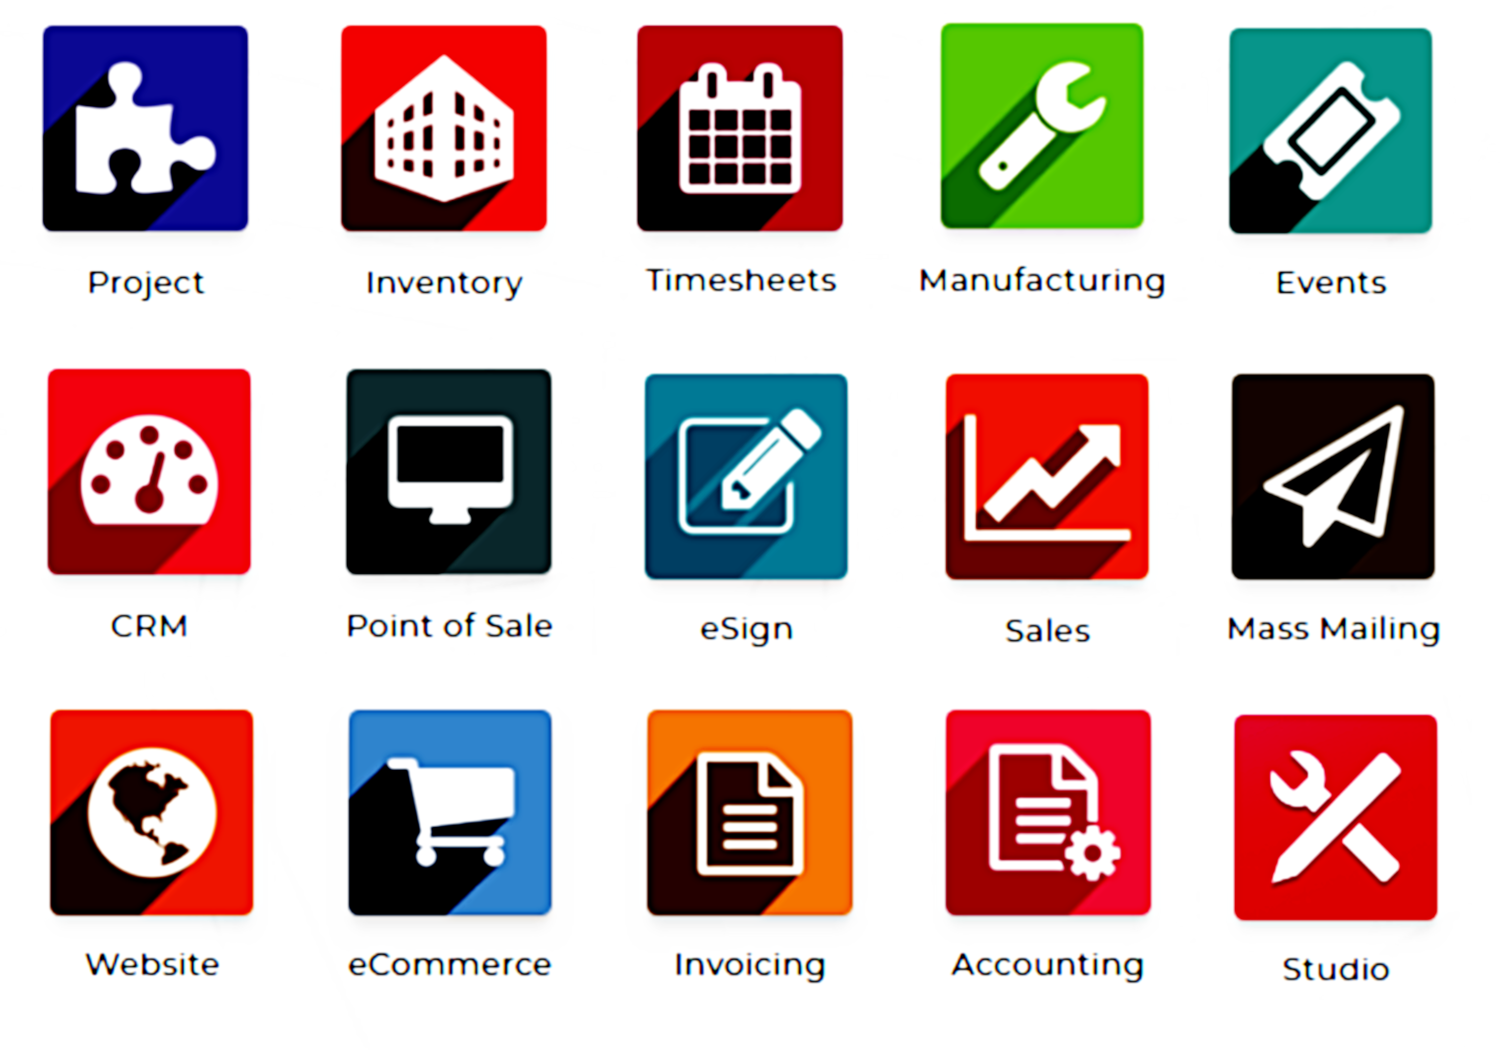
\includegraphics{images/odooerp.png}
\caption{ODOO ERP Modules}
\end{figure}

\hypertarget{projectfedena.com-an-example-of-an-erp}{%
\subsection{ProjectFedena.com: an example of an ERP}\label{projectfedena.com-an-example-of-an-erp}}

Project Fedena was conceived as a project to easily manage all campus records of schools and campuses and was implemented as a ERP system written in Ruby on Rails. The project was originally developed at Foradian Technologies but is now maintained by the open source community.\footnote{The Fedena source code can be found online at \url{https://github.com/projectfedena/fedena}}

\begin{figure}
\centering
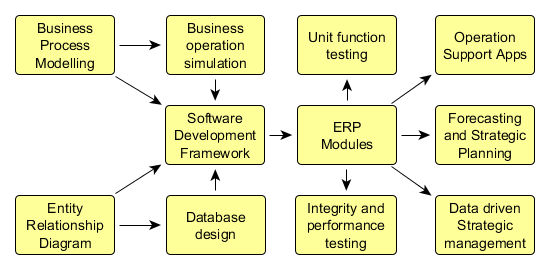
\includegraphics{images/softwaresystems.png}
\caption{Business System Software Development}
\end{figure}

\hypertarget{the-mvc-framework}{%
\subsection{The MVC Framework}\label{the-mvc-framework}}

\begin{itemize}
\tightlist
\item
  \textbf{Model:} Defines the structure and nature of data used by the system includes permissions, validation and list of field attributes.
\item
  \textbf{View:} Renders outputs according to the limitations of the media such as web, email, sms, mobile, graphic image, json and xml.
\item
  \textbf{Controller:} Parses the user request into data queries and passes the response to the appropriate view. User requests are generally variants of the standard types of database functions: create, show, edit, update and delete.
\item
  \textbf{Helpers:} calculates basic conversions including support for foreign languages.
\end{itemize}

\begin{figure}
\centering
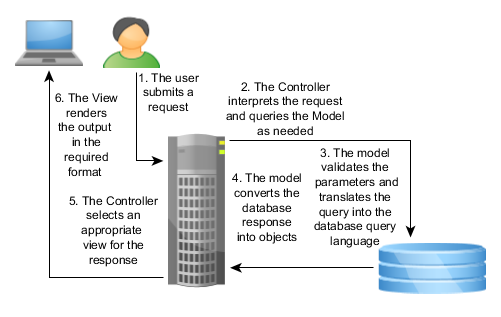
\includegraphics{images/mvc.png}
\caption{MVC Communications}
\end{figure}

The Model implements the ERD. This is example comes from the Subject Model class definition.

\begin{Shaded}
\begin{Highlighting}[]
\NormalTok{belongs_to }\StringTok{:batch}
\NormalTok{belongs_to }\StringTok{:elective_group}
\NormalTok{has_many }\StringTok{:timetable_entries}\NormalTok{,}\StringTok{:foreign_key=}\NormalTok{>}\StringTok{'subject_id'}
\NormalTok{has_many }\StringTok{:employees_subjects}
\NormalTok{has_many }\StringTok{:employees}\NormalTok{ ,}\StringTok{:through}\NormalTok{ => }\StringTok{:employees_subjects}
\NormalTok{has_many }\StringTok{:students_subjects}
\NormalTok{has_many }\StringTok{:students}\NormalTok{, }\StringTok{:through}\NormalTok{ => }\StringTok{:students_subjects}
\NormalTok{has_many }\StringTok{:grouped_exam_reports}
\NormalTok{has_and_belongs_to_many_with_deferred_save }\StringTok{:fa_groups}
\NormalTok{validates_presence_of }\StringTok{:name}\NormalTok{, }\StringTok{:max_weekly_classes}\NormalTok{, }\StringTok{:code}\NormalTok{,}\StringTok{:batch_id}
\NormalTok{validates_presence_of }\StringTok{:credit_hours}\NormalTok{,}
   \StringTok{:if=}\NormalTok{>}\StringTok{:check_grade_type}
\NormalTok{validates_numericality_of }\StringTok{:max_weekly_classes}
\NormalTok{validates_numericality_of }\StringTok{:amount}\NormalTok{,}\StringTok{:allow_nil}\NormalTok{ => }\DecValTok{true}
\NormalTok{validates_uniqueness_of }\StringTok{:code}\NormalTok{, }\StringTok{:case_sensitive}\NormalTok{ => }\DecValTok{false}
\end{Highlighting}
\end{Shaded}

\hypertarget{unit-testing}{%
\subsection{Unit testing}\label{unit-testing}}

This is done through a series of Assertions that tried against the functions of a class:

\begin{Shaded}
\begin{Highlighting}[]
\KeywordTok{class} \DataTypeTok{SimpleNumber}

   \KeywordTok{def}\NormalTok{ initialize(num)}
\NormalTok{       raise }\KeywordTok{unless}\NormalTok{ num.is_a?(}\DataTypeTok{Numeric}\NormalTok{)}
       \OtherTok{@x}\NormalTok{ = num}
   \KeywordTok{end}

   \KeywordTok{def}\NormalTok{ add(y)}
      \OtherTok{@x}\NormalTok{ + y}
   \KeywordTok{end}

   \KeywordTok{def}\NormalTok{ multiply(y)}
       \OtherTok{@x}\NormalTok{ * y}
   \KeywordTok{end}
\KeywordTok{end}
\end{Highlighting}
\end{Shaded}

\begin{Shaded}
\begin{Highlighting}[]
\NormalTok{require_relative }\StringTok{"simple_number"}
\NormalTok{require }\StringTok{"test/unit"}
     
\KeywordTok{class} \DataTypeTok{TestSimpleNumber}\NormalTok{ < }\DataTypeTok{Test}\NormalTok{::}\DataTypeTok{Unit}\NormalTok{::}\DataTypeTok{TestCase}
     
  \KeywordTok{def}\NormalTok{ test_simple}
\NormalTok{    assert_equal(}\DecValTok{4}\NormalTok{, }\DataTypeTok{SimpleNumber}\NormalTok{.new(}\DecValTok{2}\NormalTok{).add(}\DecValTok{2}\NormalTok{) )}
\NormalTok{    assert_equal(}\DecValTok{6}\NormalTok{, }\DataTypeTok{SimpleNumber}\NormalTok{.new(}\DecValTok{2}\NormalTok{).multiply(}\DecValTok{3}\NormalTok{) )}
  \KeywordTok{end}    
\KeywordTok{end}
\end{Highlighting}
\end{Shaded}

\hypertarget{available-assertions}{%
\subsection{Available assertions:}\label{available-assertions}}

\begin{longtable}[]{@{}ll@{}}
\toprule
\begin{minipage}[b]{0.43\columnwidth}\raggedright
Assertion\strut
\end{minipage} & \begin{minipage}[b]{0.51\columnwidth}\raggedright
Description\strut
\end{minipage}\tabularnewline
\midrule
\endhead
\begin{minipage}[t]{0.43\columnwidth}\raggedright
\texttt{assert(\ boolean,\ {[}message{]}\ )}\strut
\end{minipage} & \begin{minipage}[t]{0.51\columnwidth}\raggedright
True if boolean\strut
\end{minipage}\tabularnewline
\begin{minipage}[t]{0.43\columnwidth}\raggedright
\texttt{assert\_equal(\ expected,\ actual,\ {[}message{]}\ )}\strut
\end{minipage} & \begin{minipage}[t]{0.51\columnwidth}\raggedright
True if expected == actual\strut
\end{minipage}\tabularnewline
\begin{minipage}[t]{0.43\columnwidth}\raggedright
\texttt{assert\_not\_equal(\ expected,\ actual,\ {[}message{]}\ )}\strut
\end{minipage} & \begin{minipage}[t]{0.51\columnwidth}\raggedright
True if expected != actual\strut
\end{minipage}\tabularnewline
\begin{minipage}[t]{0.43\columnwidth}\raggedright
\texttt{assert\_match(\ pattern,\ string,\ {[}message{]}\ )}\strut
\end{minipage} & \begin{minipage}[t]{0.51\columnwidth}\raggedright
True if string =\textasciitilde{} pattern\strut
\end{minipage}\tabularnewline
\begin{minipage}[t]{0.43\columnwidth}\raggedright
\texttt{assert\_no\_match(\ pattern,\ string,\ {[}message{]}\ )}\strut
\end{minipage} & \begin{minipage}[t]{0.51\columnwidth}\raggedright
True if string !\textasciitilde{} pattern\strut
\end{minipage}\tabularnewline
\begin{minipage}[t]{0.43\columnwidth}\raggedright
\texttt{assert\_nil(\ object,\ {[}message{]}\ )}\strut
\end{minipage} & \begin{minipage}[t]{0.51\columnwidth}\raggedright
True if object == nil\strut
\end{minipage}\tabularnewline
\begin{minipage}[t]{0.43\columnwidth}\raggedright
\texttt{assert\_not\_nil(\ object,\ {[}message{]}\ )}\strut
\end{minipage} & \begin{minipage}[t]{0.51\columnwidth}\raggedright
True if object != nil\strut
\end{minipage}\tabularnewline
\begin{minipage}[t]{0.43\columnwidth}\raggedright
\texttt{assert\_in\_delta(\ expected\_float,\ actual\_float,\ delta,\ {[}message{]}\ )}\strut
\end{minipage} & \begin{minipage}[t]{0.51\columnwidth}\raggedright
True if (actual\_float - expected\_float).abs \textless{}= delta\strut
\end{minipage}\tabularnewline
\begin{minipage}[t]{0.43\columnwidth}\raggedright
\texttt{assert\_instance\_of(\ class,\ object,\ {[}message{]}\ )}\strut
\end{minipage} & \begin{minipage}[t]{0.51\columnwidth}\raggedright
True if object.class == class\strut
\end{minipage}\tabularnewline
\begin{minipage}[t]{0.43\columnwidth}\raggedright
\texttt{assert\_kind\_of(\ class,\ object,\ {[}message{]}\ )}\strut
\end{minipage} & \begin{minipage}[t]{0.51\columnwidth}\raggedright
True if object.kind\_of?(class)\strut
\end{minipage}\tabularnewline
\begin{minipage}[t]{0.43\columnwidth}\raggedright
\texttt{assert\_same(\ expected,\ actual,\ {[}message{]})}\strut
\end{minipage} & \begin{minipage}[t]{0.51\columnwidth}\raggedright
True if actual.equal?( expected ).\strut
\end{minipage}\tabularnewline
\begin{minipage}[t]{0.43\columnwidth}\raggedright
\texttt{assert\_not\_same(\ expected,\ actual,\ {[}message{]}\ )}\strut
\end{minipage} & \begin{minipage}[t]{0.51\columnwidth}\raggedright
True if not actual.equal?( expected ).\strut
\end{minipage}\tabularnewline
\begin{minipage}[t]{0.43\columnwidth}\raggedright
\texttt{assert\_raise(\ Exception,...\ )\ \{block\}}\strut
\end{minipage} & \begin{minipage}[t]{0.51\columnwidth}\raggedright
True if the block raises one of the listed exceptions.\strut
\end{minipage}\tabularnewline
\begin{minipage}[t]{0.43\columnwidth}\raggedright
\texttt{assert\_nothing\_raised(\ Exception,...)\ \{block\}}\strut
\end{minipage} & \begin{minipage}[t]{0.51\columnwidth}\raggedright
True if the block does not raise one of the listed exceptions.\strut
\end{minipage}\tabularnewline
\begin{minipage}[t]{0.43\columnwidth}\raggedright
\texttt{assert\_throws(\ expected\_symbol,\ {[}message{]}\ )\ \{block\}}\strut
\end{minipage} & \begin{minipage}[t]{0.51\columnwidth}\raggedright
\strut
\end{minipage}\tabularnewline
\begin{minipage}[t]{0.43\columnwidth}\raggedright
\texttt{assert\_nothing\_thrown(\ {[}message{]}\ )\ \{block\}}\strut
\end{minipage} & \begin{minipage}[t]{0.51\columnwidth}\raggedright
True if the block throws (or doesn't) the expected\_symbol.\strut
\end{minipage}\tabularnewline
\begin{minipage}[t]{0.43\columnwidth}\raggedright
\texttt{assert\_respond\_to(\ object,\ method,\ {[}message{]}\ )}\strut
\end{minipage} & \begin{minipage}[t]{0.51\columnwidth}\raggedright
True if the object can respond to the given method.\strut
\end{minipage}\tabularnewline
\begin{minipage}[t]{0.43\columnwidth}\raggedright
\texttt{assert\_send(\ send\_array,\ {[}message{]}\ )}\strut
\end{minipage} & \begin{minipage}[t]{0.51\columnwidth}\raggedright
True if the method sent to the object with the given arguments return true.\strut
\end{minipage}\tabularnewline
\begin{minipage}[t]{0.43\columnwidth}\raggedright
\texttt{assert\_operator(\ object1,\ operator,\ object2,\ {[}message{]}\ )}\strut
\end{minipage} & \begin{minipage}[t]{0.51\columnwidth}\raggedright
Compares the two objects with the given operator, passes if true\strut
\end{minipage}\tabularnewline
\bottomrule
\end{longtable}

\hypertarget{behavior-driven-development}{%
\section{Behavior driven Development}\label{behavior-driven-development}}

Advantages:

\begin{itemize}
\tightlist
\item
  \textbf{Single source of truth:} Specifications, tests and documentation are in the same document.
\item
  \textbf{Living documentation:} Because they're automatically tested by Cucumber, your specifications are always bang up-to-date.
\item
  \textbf{Customer focus:} Cucumber helps business and IT collaborate to build a shared understanding of the business goals
\end{itemize}

\citep{Cucumber2019a} supports Behaviour-Driven Development(BDD) by reading executable specifications written in plain text and validating that the software does what those specifications say. The specifications consists of multiple examples, or scenarios written in Gherkin. \citep{Cucumber2019b}

The primary keywords are:

\begin{itemize}
\item
  \texttt{Feature}
\item
  \texttt{Example} (\texttt{Scenario} and \texttt{Scenario\ Outline} are synonyms)
\item
  Steps: \texttt{Given}, \texttt{When}, \texttt{Then}, \texttt{And}, \texttt{But}
\item
  \texttt{Background}
\item
  \texttt{Combinations} (Examples is a synonum)
\item
  \texttt{"..."} (Doc Strings)
\item
  \texttt{\textbar{}} (Data Tables)
\item
  \texttt{@} (Tags)
\item
  \texttt{\#} (Comments)
\end{itemize}

Examples follow this same pattern:

\begin{itemize}
\tightlist
\item
  Describe an initial context (Given steps)
\item
  Describe an event (When steps)
\item
  Describe an expected outcome (Then steps)
\end{itemize}

\hypertarget{a-working-example-of-specs-in-cucumber}{%
\subsection{A working example of specs in Cucumber}\label{a-working-example-of-specs-in-cucumber}}

\begin{Shaded}
\begin{Highlighting}[]
\DataTypeTok{Feature}\NormalTok{: A simple banking program}
        
\DataTypeTok{Background}\NormalTok{:}
   \DataTypeTok{Given}\NormalTok{ a customer named }\StringTok{"DrBob"}          
   \DataTypeTok{And}\NormalTok{ I have logged }\KeywordTok{in}\NormalTok{ as }\StringTok{"DrBob"}    

   \DataTypeTok{Scenario}\NormalTok{: }\DataTypeTok{Balance}\NormalTok{ checking   }
   \DataTypeTok{Given}\NormalTok{ my account has a balance of }\DataTypeTok{$430}   
   \DataTypeTok{Then}\NormalTok{ my account should show a balance of }\DataTypeTok{$430}   
           
   \DataTypeTok{Scenario}\NormalTok{: }\DataTypeTok{Account}\NormalTok{ deposit   }
   \DataTypeTok{Given}\NormalTok{ my account has a balance of }\DataTypeTok{$400}   
   \DataTypeTok{When}\NormalTok{ I deposit }\DataTypeTok{$30}   
   \DataTypeTok{Then}\NormalTok{ my account should show a balance of }\DataTypeTok{$430}   
         
   \DataTypeTok{Scenario}\NormalTok{: }\DataTypeTok{Account}\NormalTok{ withdraw   }
   \DataTypeTok{Given}\NormalTok{ my account has a balance of }\DataTypeTok{$500}
   \DataTypeTok{When}\NormalTok{ I withdraw }\DataTypeTok{$70}
   \DataTypeTok{Then}\NormalTok{ my account should show a balance of }\DataTypeTok{$430}     
         
   \DataTypeTok{Scenario} \DataTypeTok{Outline}\NormalTok{: deposits   }
   \DataTypeTok{Given}\NormalTok{ there are <start> dollars }\KeywordTok{in}\NormalTok{ the account   }
   \DataTypeTok{When}\NormalTok{ I deposit <added> dollars   }
   \DataTypeTok{Then}\NormalTok{ I should have <left> dollars   }
     
   \DataTypeTok{Examples}\NormalTok{:    }
\NormalTok{     | start | added | left |   }
\NormalTok{     |    }\DecValTok{12}\NormalTok{ |   }\DecValTok{5}\NormalTok{   |    }\DecValTok{7}\NormalTok{ |   }
\NormalTok{     |    }\DecValTok{20}\NormalTok{ |   }\DecValTok{5}\NormalTok{   |   }\DecValTok{15}\NormalTok{ |   }
\end{Highlighting}
\end{Shaded}

\hypertarget{business-software-systems}{%
\chapter{BUSINESS SOFTWARE SYSTEMS}\label{business-software-systems}}

\begin{figure}
\centering
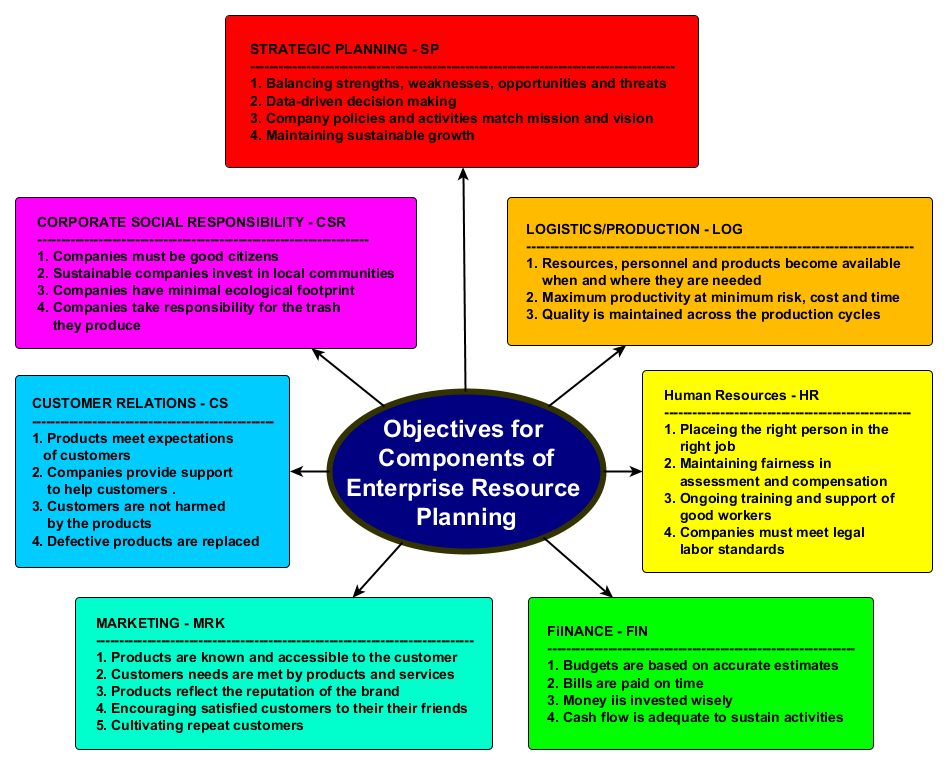
\includegraphics{images/ebusiness.png}
\caption{Objectives of ERP Components}
\end{figure}

\hypertarget{online-store}{%
\section{Online Store}\label{online-store}}

An online store attempts to match or exceed the level of customer support provided in brick and mortar stores. However, the personal distance and anonymity of the internet makes this goal harder to achieve. However, online stores like Amazon, Lazada and Alibaba owe their success to their ability to create trust among their community of buyers and sellers. These companies act as arbitrators between customers and vendors, reducing the risk of doing business between unkonwn parties. B ecause trust is so essential to business transactions, many internet shops began as product listings on one of these large marketing sysems, or as a online service to the customers of their brick and mortar chains.

\hypertarget{stages-in-customer-purchasing-decisions}{%
\subsection{Stages in Customer Purchasing Decisions}\label{stages-in-customer-purchasing-decisions}}

Marketers have long studied the process and requirements of customers before, during and after making a purchase. In a market place that abound in choices, customers must choose between the multiple alternatives. Shopping whether in the physical world or online is at best weak attempt at making a rational decision between the choices, because complete analysis needed to identify the true optimal decision is increditably complex. \citep{Simon1955} However, the urgency of the need drives the buyer to settle for an apparent good choice. However, the internet changes this by providing more information on which to base a rational decision. \citep{Dewey1910} observed 5 stages in a purchasing decision. A sixth stage has been added here to cover the financial transaction constraints imposed by online monetary systems.

\begin{figure}
\centering
\includegraphics{images/purchase.png}
\caption{Stages in customer purchase decision making}
\end{figure}

\hypertarget{business-processes-to-support-shoppers}{%
\subsection{Business Processes to Support Shoppers}\label{business-processes-to-support-shoppers}}

\begin{figure}
\centering
\includegraphics{images/onlinesales.png}
\caption{Business support of shoppers}
\end{figure}

\hypertarget{steps-of-check-out-and-order-fulfillment}{%
\subsection{Steps of check out and order fulfillment}\label{steps-of-check-out-and-order-fulfillment}}

\begin{itemize}
\tightlist
\item
  Login: links to shopping cart and history

  \begin{itemize}
  \tightlist
  \item
    Establish an account with the vendor
  \item
    Add items to the shopping cart
  \end{itemize}
\item
  Shopping cart check out

  \begin{itemize}
  \tightlist
  \item
    Conducts an inventory check of items in shopping cart
  \item
    Determines the mode of shipping
  \item
    Calculates bill
  \end{itemize}
\item
  Renumeration via bank transfer

  \begin{itemize}
  \tightlist
  \item
    Determines the method of payment
  \item
    Login onto financial service
  \item
    Confirms the transaction
  \item
    SMS validation code to telephone
  \item
    Conducts and records the transaction
  \item
    Send payment confirmation to the vendor
  \end{itemize}
\end{itemize}

\BeginKnitrBlock{rmdextra}
** Online Payment Methods Used in Thailand

Credit card and bank fraud so common in Thailand that most banks and credit card companies do not provide the quarantees for purchases and other consumer protection that conhsumers in other countries enjoy. In essence, Thai financial firms assume no risk and carry no insuraNCE against bank and credit card fraud. Despite the barriers against credit card usage, there are online payment systems used for e-commerce in Thailand as shown in the following table.

\begin{longtable}[]{@{}lll@{}}
\toprule
\begin{minipage}[b]{0.28\columnwidth}\raggedright
Type and example\strut
\end{minipage} & \begin{minipage}[b]{0.30\columnwidth}\raggedright
Benefits\strut
\end{minipage} & \begin{minipage}[b]{0.34\columnwidth}\raggedright
Drawbacks\strut
\end{minipage}\tabularnewline
\midrule
\endhead
\begin{minipage}[t]{0.28\columnwidth}\raggedright
\textbf{Credit card}\strut
\end{minipage} & \begin{minipage}[t]{0.30\columnwidth}\raggedright
Convenient, international standard\strut
\end{minipage} & \begin{minipage}[t]{0.34\columnwidth}\raggedright
\strut
\end{minipage}\tabularnewline
\begin{minipage}[t]{0.28\columnwidth}\raggedright
\textbf{Bank transfer}\strut
\end{minipage} & \begin{minipage}[t]{0.30\columnwidth}\raggedright
\strut
\end{minipage} & \begin{minipage}[t]{0.34\columnwidth}\raggedright
\strut
\end{minipage}\tabularnewline
\begin{minipage}[t]{0.28\columnwidth}\raggedright
\textbf{ATM}\strut
\end{minipage} & \begin{minipage}[t]{0.30\columnwidth}\raggedright
\strut
\end{minipage} & \begin{minipage}[t]{0.34\columnwidth}\raggedright
\strut
\end{minipage}\tabularnewline
\begin{minipage}[t]{0.28\columnwidth}\raggedright
\textbf{Online payment company:} Paypal, Alipay\strut
\end{minipage} & \begin{minipage}[t]{0.30\columnwidth}\raggedright
\strut
\end{minipage} & \begin{minipage}[t]{0.34\columnwidth}\raggedright
\strut
\end{minipage}\tabularnewline
\begin{minipage}[t]{0.28\columnwidth}\raggedright
\textbf{Payment service} 7-Eleven, Thailand Postal Service\strut
\end{minipage} & \begin{minipage}[t]{0.30\columnwidth}\raggedright
\strut
\end{minipage} & \begin{minipage}[t]{0.34\columnwidth}\raggedright
The payment collection service charges the vendor a high commission and their systems could be hacked.\strut
\end{minipage}\tabularnewline
\begin{minipage}[t]{0.28\columnwidth}\raggedright
\textbf{Mobile phone credits} AIS, TOT\strut
\end{minipage} & \begin{minipage}[t]{0.30\columnwidth}\raggedright
\strut
\end{minipage} & \begin{minipage}[t]{0.34\columnwidth}\raggedright
Reimbursement depends on the policies of the phone company; Stolen phone transactions may have to be refunded.\strut
\end{minipage}\tabularnewline
\begin{minipage}[t]{0.28\columnwidth}\raggedright
\textbf{Cash on delivery:} Lazada\strut
\end{minipage} & \begin{minipage}[t]{0.30\columnwidth}\raggedright
\strut
\end{minipage} & \begin{minipage}[t]{0.34\columnwidth}\raggedright
The receiver can refuse the delivery and the goods are returned damaged in shipment\strut
\end{minipage}\tabularnewline
\begin{minipage}[t]{0.28\columnwidth}\raggedright
\textbf{Cryptocurrency:} BitCoin\strut
\end{minipage} & \begin{minipage}[t]{0.30\columnwidth}\raggedright
\strut
\end{minipage} & \begin{minipage}[t]{0.34\columnwidth}\raggedright
The market value is not pegged to that of physical currency\strut
\end{minipage}\tabularnewline
\bottomrule
\end{longtable}
\EndKnitrBlock{rmdextra}

\begin{itemize}
\tightlist
\item
  Send a shipping request to the Fulfillment Center

  \begin{itemize}
  \tightlist
  \item
    Pick list and shipping manifest
  \item
    Print shipping label
  \item
    Send pick up order to delivery service
  \end{itemize}
\item
  Shipping

  \begin{itemize}
  \tightlist
  \item
    Record shipment pickup
  \item
    Register the shipment
  \item
    Track the shipment
  \item
    Record the delivery
  \end{itemize}
\end{itemize}

\hypertarget{customer-relations-management}{%
\section{Customer Relations Management}\label{customer-relations-management}}

\hypertarget{post-sales-service}{%
\subsection{Post sales service}\label{post-sales-service}}

\begin{itemize}
\tightlist
\item
  Unpacking instructions
\item
  Installation instructions
\item
  User instructions
\item
  Troubleshooting guide
\item
  Technical support hotline
\item
  Service center locations
\end{itemize}

\hypertarget{measuring-the-effectiveness-of-websites}{%
\section{Measuring the effectiveness of websites}\label{measuring-the-effectiveness-of-websites}}

\hypertarget{human-resources-management}{%
\section{Human Resources Management}\label{human-resources-management}}

\hypertarget{assessing-personal-temperment}{%
\subsection{Assessing Personal Temperment}\label{assessing-personal-temperment}}

Every person is unique and represents a unique set of strengths and weaknesses. At the same time the every job requires different set of characteristics. The role of HR is to attempt to collectin information meant to measure and ascertain how suited an applicant is for a job opening. In theory the goal is to play the right person in the job. However as implied by the following word cloud, fitness of applicants for a job has many dimensions and is hard to measure accurately.

\begin{figure}
\centering
\includegraphics{images/wordcloud.png}
\caption{Characteristics of a Good Employee}
\end{figure}

\BeginKnitrBlock{rmdexercise}
\textbf{Exercise: Employee selection criteria}

The following are redacted from ads for IT jobs in Chiang Mai posted on LinkedIn in 2018. For each of the job descriptions propose the top 4 characteristics that should be used to identify a suitable candidate:

\begin{enumerate}
\def\labelenumi{\arabic{enumi}.}
\tightlist
\item
  \textbf{Software Developer:} At XXX, we pursue greatness for our clients while reaching our own potential as well. To achieve this, we are building a team of people who can work independently, who push themselves to find creative solutions, who collaborate naturally, and who, above all, value doing good work. We are looking for new members for our team who can craft web and mobile applications that fit inside a larger communications, business, and product strategies. We focus on the problems to be solved instead of lists of functional requirements. The applications we develop are always part of larger strategy and help us foster close partnerships with our clients and the users of our applications. Together we work to amplify the effectiveness of our clients and accelerate their growth.
\item
  \textbf{Data scientist:} At YYY, we work closely with business users to identify business problems and develop solutions using data science techniques. To this end, we design and implement data models to explain and solve critical problems using such techniques as data mining, statistical modeling, and machine learning. We are looking for a worker who can provide insightful visualization and explanation of trends in client data and recommend the next course of action to be taken by decision makers and their colleagues.
\item
  \textbf{Robotics Engineer:} We are seeking a Robotic Engineer with technical leadership expertise to optimize the expansion of our paint robot program by improving the efficiency, productivity and quality of our program. You will be responsible for program operation, fault recovery procedures, troubleshooting and all around leadership of a state-of-the-art program to triple the paint volume of our previous model. In addition, you will contribute to improvements in Robot Safety, graphic user interface, electrostatic paint application, robot pathing, robotic fluid delivery systems, and the training of the next generation of program operators.
\item
  \textbf{Solutions Architect:} At WWW, we are looking for someone with a passion to help customers design large distributed systems using the world's most advanced cloud computing technologies. This job requires someone who can communicate, consult, and provide leadership while helping to guide major projects to success. We are hiring a Solutions Architect who can think strategically about business, product, and technical challenges and who will own technical engagement with customers on projects, working cross-organizationally to facilitate adoption and use of the cloud platform. At the same time, the job will involve developing a deep expertise in the cloud technologies and contributing to the know-how in the construction of applications and services on the cloud platform.
\end{enumerate}
\EndKnitrBlock{rmdexercise}

\hypertarget{belbin-team-roles}{%
\subsubsection{Belbin Team Roles}\label{belbin-team-roles}}

Research showed that the most successful teams were made up of a diverse mix of behaviours; they had access to all nine Belbin Team Roles. A Team Role was defined by Dr Meredith Belbin as ``A tendency to behave, contribute and interrelate with others in a particular way''. The value of Belbin Team Role theory lies in enabling an individual or team to benefit from self knowledge and adjust according to the demands being made by the external situation. \citep{Belbin2010} The concept was derived from a study of factors leading to success or failure of teams competing in
Business Games at Henley Management College, England. Managers taking part in the exercise
were given a battery of psychometric tests and put into teams of varying composition. As time
progressed different clusters of behaviour were identified as underlying the success of the teams. These successful clusters of behaviour were then given names. Hence the emergence of nine Team Roles shown with the distribution among British managers: \citep{Fisher1998}

\begin{longtable}[]{@{}lccc@{}}
\toprule
Roles & & Belbin Types &\tabularnewline
\midrule
\endhead
Action-oriented: & Shaper & Implementer & Completer Finisher\tabularnewline
& 2.3\% & 11.4\% & 3.6\%\tabularnewline
People-oriented: & Co-ordinator & Teamworker & Resource Investigator\tabularnewline
& 26.2\% & 18.2\% & 33.2\%\tabularnewline
Thinking-oriented: & Plant & Monitor Evaluator & Specialist\tabularnewline
& 3.7\% & 0.5\% & 0.8\%\tabularnewline
\bottomrule
\end{longtable}

This doesn't mean that every team requires nine people. Most people will have two or three Team Roles that they are most comfortable with. Team Roles develop and mature. These may change with experience and conscious attention. Different Team Roles may come to the fore in response to the needs of particular situations.

\begin{longtable}[]{@{}llll@{}}
\toprule
\begin{minipage}[b]{0.21\columnwidth}\raggedright
Role Description\strut
\end{minipage} & \begin{minipage}[b]{0.25\columnwidth}\raggedright
Strengths\strut
\end{minipage} & \begin{minipage}[b]{0.20\columnwidth}\raggedright
Allowable weaknesses\strut
\end{minipage} & \begin{minipage}[b]{0.22\columnwidth}\raggedright
Concerns\strut
\end{minipage}\tabularnewline
\midrule
\endhead
\begin{minipage}[t]{0.21\columnwidth}\raggedright
\textbf{Resource Investigator:} Uses their inquisitive nature to find ideas to bring back to the team.\strut
\end{minipage} & \begin{minipage}[t]{0.25\columnwidth}\raggedright
Outgoing, enthusiastic. Explores opportunities and develops contacts.\strut
\end{minipage} & \begin{minipage}[t]{0.20\columnwidth}\raggedright
Might be over-optimistic, and can lose interest once the initial enthusiasm has passed.\strut
\end{minipage} & \begin{minipage}[t]{0.22\columnwidth}\raggedright
They might forget to follow up on a lead.\strut
\end{minipage}\tabularnewline
\begin{minipage}[t]{0.21\columnwidth}\raggedright
\textbf{Teamworker:} Helps the team to gel, using their versatility to identify the work required and complete it on behalf of the team.\strut
\end{minipage} & \begin{minipage}[t]{0.25\columnwidth}\raggedright
Co-operative, perceptive and diplomatic. Listens and averts friction.\strut
\end{minipage} & \begin{minipage}[t]{0.20\columnwidth}\raggedright
Can be indecisive in crunch situations and tends to avoid confrontation.\strut
\end{minipage} & \begin{minipage}[t]{0.22\columnwidth}\raggedright
They might hesitate to make unpopular decisions.\strut
\end{minipage}\tabularnewline
\begin{minipage}[t]{0.21\columnwidth}\raggedright
\textbf{Co-ordinator:} Needed to focus on the team's objectives, draw out team members and delegate work appropriately.\strut
\end{minipage} & \begin{minipage}[t]{0.25\columnwidth}\raggedright
Mature, confident, identifies talent. Clarifies goals.\strut
\end{minipage} & \begin{minipage}[t]{0.20\columnwidth}\raggedright
Can be seen as manipulative and might offload their own share of the work.\strut
\end{minipage} & \begin{minipage}[t]{0.22\columnwidth}\raggedright
They can over-delegate, leaving themselves little work to do.\strut
\end{minipage}\tabularnewline
\begin{minipage}[t]{0.21\columnwidth}\raggedright
\textbf{Plant:} Tends to be highly creative and good at solving problems in unconventional ways.\strut
\end{minipage} & \begin{minipage}[t]{0.25\columnwidth}\raggedright
Creative, imaginative, free-thinking, generates ideas and solves difficult problems.\strut
\end{minipage} & \begin{minipage}[t]{0.20\columnwidth}\raggedright
Might ignore incidentals, and may be too preoccupied to communicate effectively.\strut
\end{minipage} & \begin{minipage}[t]{0.22\columnwidth}\raggedright
They could be absent-minded and forgetful.\strut
\end{minipage}\tabularnewline
\begin{minipage}[t]{0.21\columnwidth}\raggedright
\textbf{Monitor Evaluator:} Provides a logical eye, making impartial judgements where required and weighs up the team's options\strut
\end{minipage} & \begin{minipage}[t]{0.25\columnwidth}\raggedright
Sober, strategic and discerning. Sees all options and judges accurately.\strut
\end{minipage} & \begin{minipage}[t]{0.20\columnwidth}\raggedright
Sometimes lacks the drive in a dispassionate way. and ability to inspire others and can be overly critical.\strut
\end{minipage} & \begin{minipage}[t]{0.22\columnwidth}\raggedright
They could be slow to come to decisions.\strut
\end{minipage}\tabularnewline
\begin{minipage}[t]{0.21\columnwidth}\raggedright
\textbf{Specialist:} Brings in-depth knowledge of a key area to the team.\strut
\end{minipage} & \begin{minipage}[t]{0.25\columnwidth}\raggedright
Single-minded, self-starting and dedicated. They provide specialist knowledge and skills.\strut
\end{minipage} & \begin{minipage}[t]{0.20\columnwidth}\raggedright
Tends to contribute on a narrow front and can dwell on the technicalities.\strut
\end{minipage} & \begin{minipage}[t]{0.22\columnwidth}\raggedright
They can overload colleagues with technical information.\strut
\end{minipage}\tabularnewline
\begin{minipage}[t]{0.21\columnwidth}\raggedright
\textbf{Shaper:} Provides the necessary drive to ensure that the team keeps moving and does not lose focus or momentum.\strut
\end{minipage} & \begin{minipage}[t]{0.25\columnwidth}\raggedright
Challenging, dynamic, thrives on pressure. Has the drive and courage to overcome obstacles.\strut
\end{minipage} & \begin{minipage}[t]{0.20\columnwidth}\raggedright
Can be prone to provocation, and may sometimes offend people's feelings.\strut
\end{minipage} & \begin{minipage}[t]{0.22\columnwidth}\raggedright
They could risk becoming aggressive and bad-humoured in their attempts to get things done.\strut
\end{minipage}\tabularnewline
\begin{minipage}[t]{0.21\columnwidth}\raggedright
\textbf{Implementer:} Needed to plan a workable strategy and carry it out as efficiently as possible.\strut
\end{minipage} & \begin{minipage}[t]{0.25\columnwidth}\raggedright
Practical, reliable, efficient. Turns ideas into actions and organises work that needs to be done.\strut
\end{minipage} & \begin{minipage}[t]{0.20\columnwidth}\raggedright
Can be a bit inflexible and slow to respond to new possibilities.\strut
\end{minipage} & \begin{minipage}[t]{0.22\columnwidth}\raggedright
They might be slow to relinquish their plans in favour of positive changes.\strut
\end{minipage}\tabularnewline
\begin{minipage}[t]{0.21\columnwidth}\raggedright
\textbf{Completer Finisher:} Most effectively used at the end of tasks to polish and scrutinise the work for errors, subjecting it to the highest standards of quality control.\strut
\end{minipage} & \begin{minipage}[t]{0.25\columnwidth}\raggedright
Painstaking, conscientious, anxious. Searches out errors. Polishes and perfects.\strut
\end{minipage} & \begin{minipage}[t]{0.20\columnwidth}\raggedright
Can be inclined to worry unduly, and reluctant to delegate.\strut
\end{minipage} & \begin{minipage}[t]{0.22\columnwidth}\raggedright
They could be accused of taking their perfectionism to extremes.\strut
\end{minipage}\tabularnewline
\bottomrule
\end{longtable}

\hypertarget{big-5-behavioral-types}{%
\subsubsection{Big 5 Behavioral Types}\label{big-5-behavioral-types}}

\begin{longtable}[]{@{}lll@{}}
\toprule
\begin{minipage}[b]{0.44\columnwidth}\raggedright
Behavioral Characteristic\strut
\end{minipage} & \begin{minipage}[b]{0.28\columnwidth}\raggedright
Low end\strut
\end{minipage} & \begin{minipage}[b]{0.20\columnwidth}\raggedright
High end\strut
\end{minipage}\tabularnewline
\midrule
\endhead
\begin{minipage}[t]{0.44\columnwidth}\raggedright
\textbf{Openness to experience:} Appreciation for art, emotion, adventure, unusual ideas curiosity, variety of experience and intellectual curiosity, creativity and a preference for novelty and variety.\strut
\end{minipage} & \begin{minipage}[t]{0.28\columnwidth}\raggedright
consistent, cautious (Accountants)\strut
\end{minipage} & \begin{minipage}[t]{0.20\columnwidth}\raggedright
inventive, curious(Artists)\strut
\end{minipage}\tabularnewline
\begin{minipage}[t]{0.44\columnwidth}\raggedright
\textbf{Conscientiousness:} A tendency to be organized and dependable, show self-discipline, act dutifully, aim for achievement, and prefer planned rather than spontaneous behavior.\strut
\end{minipage} & \begin{minipage}[t]{0.28\columnwidth}\raggedright
easy-going, careless, sloppy. (Graffiti artist)\strut
\end{minipage} & \begin{minipage}[t]{0.20\columnwidth}\raggedright
efficient, organized, stubborn. (Engraver)\strut
\end{minipage}\tabularnewline
\begin{minipage}[t]{0.44\columnwidth}\raggedright
\textbf{Extraversion:} Energy, positive emotions, surgency, assertiveness, sociability and the tendency to seek stimulation in the company of others, talkativeness and is often perceived as attention-seeking and domineering.\strut
\end{minipage} & \begin{minipage}[t]{0.28\columnwidth}\raggedright
solitary, reserved, shy, introvert. (Hermit)\strut
\end{minipage} & \begin{minipage}[t]{0.20\columnwidth}\raggedright
outgoing, energetic, boisterous, extravert. (Cheerleader)\strut
\end{minipage}\tabularnewline
\begin{minipage}[t]{0.44\columnwidth}\raggedright
\textbf{Agreeableness:} A tendency to be compassionate and cooperative rather than suspicious and antagonistic towards others. It related to a trusting and helpful nature.\strut
\end{minipage} & \begin{minipage}[t]{0.28\columnwidth}\raggedright
challenging, detached, rigid. (Prosecutor)\strut
\end{minipage} & \begin{minipage}[t]{0.20\columnwidth}\raggedright
friendly, compassionate, helpful. (Social worker)\strut
\end{minipage}\tabularnewline
\begin{minipage}[t]{0.44\columnwidth}\raggedright
\textbf{Neuroticism:} Neuroticism identifies certain people who are more prone to psychological stress and a tendency to experience unpleasant emotions easily.\strut
\end{minipage} & \begin{minipage}[t]{0.28\columnwidth}\raggedright
confident\strut
\end{minipage} & \begin{minipage}[t]{0.20\columnwidth}\raggedright
secure, cool (Air traffic controller)\strut
\end{minipage}\tabularnewline
\bottomrule
\end{longtable}

\hypertarget{myers-briggs-test}{%
\subsubsection{Myers Briggs Test}\label{myers-briggs-test}}

The 16 personality types that were developed by Isabel Briggs Myers and Katharine Cook Briggs, which was built on the work of Carl Jung in the early 1900s. Based on the 4 dimensions of Carl Jung's theory of personality types:

\begin{longtable}[]{@{}ll@{}}
\toprule
Dimension & Extremes\tabularnewline
\midrule
\endhead
Energizes & Extroversion (E) vs Internal (I)\tabularnewline
Perceives information & Sensing (S) vs Intuitive (N)\tabularnewline
Decision making & Thinking (T) vs Feeling (F)\tabularnewline
World view & Judging (J) vs Perceiving (P)\tabularnewline
\bottomrule
\end{longtable}

Myers Briggs Test has been administered to a large number of people helping to validate the value of this instrument for a number of applications. Generally successful workers tend to gravitate to specific careers based on their personality profile as shown in the next sections. \citep{Tieger2014}

\hypertarget{analysts}{%
\paragraph{Analysts:}\label{analysts}}

\begin{itemize}
\item
  \textbf{INTJ} (2.1\%) - The Mastermind/The Scientist -- Independent, original, analytical, and determined with an exceptional ability to turn theories into solid plans of action. Creative perfectionists who prefer to do things their own way, INTJs perform well in non-social roles that require them to think theoretically. Common careers: Investment banker, Personal financial advisor, Software developer, Economist, Executive
\item
  \textbf{INTP} (3.3\%) - The Thinker -- Logical, original, creative thinkers. Can become very excited about theories and ideas. Independent and creative problem-solvers, INTPs gravitate toward roles that require them to be theoretical and precise. Common careers - Computer programmer, software designer, Financial analyst, Architect, College professor, Economist
\item
  \textbf{ENTJ} (1.8\%) - The Commander -- Assertive and outspoken - they are driven to lead. Excellent ability to understand difficult organizational problems and create solid solutions. Natural leaders who are logical, analytical, and good strategic planners, ENTJs gravitate toward authoritarian roles that require them to be organized and efficient. Common careers: Executive, Lawyer, Market research analyst, Management consultant, Venture capitalist
\item
  \textbf{ENTP} (3.2\%) - The Debater -- Creative, resourceful, and intellectually quick. Good at a broad range of things. Enterprising creative people who enjoy new challenges, ENTPs excel in risky roles that require them to be persistent and non-conformist. Common careers: Entrepreneur, Real estate developer, Advertising creative director, Marketing director, Politician/political consultant
\end{itemize}

\hypertarget{diplomats}{%
\paragraph{Diplomats:}\label{diplomats}}

\begin{itemize}
\item
  \textbf{INFJ} (1.5\%) - The Counselor/The Protector -- Quietly forceful, original, and sensitive. Tend to stick to things until they are done. Thoughtful, creative people driven by firm principles and personal integrity, INFJs do well in behind-the-scenes roles that require them to communicate on a personal level. Common careers: Therapist/counsellor, Social worker, HR diversity manager, Organization development consultant, Customer relations manager
\item
  \textbf{INFP} (4.4\%) - The Idealist -- Quiet, reflective, and idealistic. Interested in serving humanity. Sensitive idealists motivated by their deeper personal values, INFPs excel in roles that require them to be compassionate and adaptable. Common careers: Graphic designer, Psychologist/therapist, Writer/editor, Physical therapist, HR development trainer
\item
  \textbf{ENFJ} (2.5\%) - The Giver -- Popular and sensitive, with outstanding people skills. Externally focused, with real concern for how others think and feel. People-lovers who are energetic, articulate, and diplomatic, ENFJs excel in cooperative roles that require them to be expressive and logical. Common careers: Advertising executive, Public relations specialist, Corporate coach/trainer, Sales manager, Employment/HR specialist
\item
  \textbf{ENFP} (8.1\%) - The Champion/The Inspirer -- Enthusiastic, idealistic, and creative. Able to do almost anything that interests them. Curious and confident creative types who see possibilities everywhere, ENFPs perform well in expressive roles that require them to be alert and communicative. Common careers: Journalist, Advertising creative director, Consultant, Restaurateur, Event planner
\end{itemize}

\hypertarget{sentinels}{%
\paragraph{Sentinels:}\label{sentinels}}

\begin{itemize}
\item
  \textbf{ISTJ} (11.6\%) - The Inspector/The Duty Fulfiller - Serious and quiet, interested in security and peaceful living. Hard workers who value their responsibilities and commitments, ISTJs excel in behind-the-scenes roles that require them to be reliable. Common careers: Auditor, Accountant, Chief financial officer, Web development engineer, Government employee
\item
  \textbf{ISFJ} (13.8\%) - The Nurturer/ -- Quiet, kind, and conscientious, puts the needs of others above self-interest. Modest and determined workers who enjoy helping others, ISFJs do well in roles that require them to provide services to others without being in a position of authority. Common careers: Dentist, Elementary school teacher, Librarian, Franchise owner, Customer service representative
\item
  \textbf{ESTJ} (8.7\%) - The Supervisor/The Guardian -- Practical, traditional, and organized. Likely to be athletic. Realists who are quick to make practical decisions, ESTJs perform well in social roles that require them to lead. Common careers: Insurance sales agent, Pharmacist, Lawyer, Judge, Project manager
\item
  \textbf{ESFJ} (12.3\%) - The Provider/The Caregiver -- Warm-hearted, popular, and conscientious. Tend to put the needs of others over self-interest. Gregarious traditionalists motivated to help others, ESFJs gravitate toward social roles that require them to care for the well-being of others. Common careers: Sales representative, Nurse/healthcare worker, Social worker, Public relations account executive, Loan officer
\end{itemize}

\hypertarget{explorers}{%
\paragraph{Explorers:}\label{explorers}}

\begin{itemize}
\item
  \textbf{ISTP} (5.4\%) - The Craftsman / The Mechanic - Quiet and reserved, interested in how and why things work. Straightforward and honest people who prefer action to conversation, ISTPs perform well in utilitarian roles that require them to make use of tools. Common careers: Civil engineer, Economist, Pilot, Data communications analysis, Emergency room physician
\item
  \textbf{ISFP} (8.8\%)- The Composer/The Artist -- Quiet, serious, sensitive and kind, avoids conflict. Warm and sensitive types who like to help people in tangible ways, ISFPs do well in roles that require them to be sympathetic and attentive. Common careers: Fashion designer, Physical therapist, Massage therapist, Landscape architect, Storekeeper
\item
  \textbf{ESTP} (4.3\%) - The Doer -- Friendly, adaptable, action-oriented. focused on immediate results. Pragmatists who love excitement and excel in a crisis, ESTPs excel in high-stakes roles that require them to be resourceful. Common careers: Detective, Banker, Investor, Entertainment agent, Sports coach
\item
  \textbf{ESFP} (8.5\%) - The Performer -- People-oriented and fun-loving, they make things more fun for others by their enjoyment. Lively and playful people who value common sense, ESFPs gravitate toward roles that require them to be expressive and interact with others. Common careers: Child welfare counselor, Primary care physician, Actor, Interior designer, Environmental scientist
\end{itemize}

\hypertarget{hofstede-survey-on-cultural-dimensions}{%
\subsubsection{Hofstede survey on cultural dimensions}\label{hofstede-survey-on-cultural-dimensions}}

By studing expat workers work preformance in large multinational corporations, Hofstede was able to identify key cultural differences in the way people approach work. \citep{Hofstede2010}

\begin{itemize}
\tightlist
\item
  Power distance: perceived ability to make a difference
\item
  Individualism: individual vs collective: tendency to think in terms of I vs We.
\item
  Gender balance: masculinity vs femininity
\item
  Advoidance of Uncertianty: tolerance of risk
\item
  Long term orientation: perception of urgency\\
\item
  Indulgences vs restraint: attitude towards acquired wealth
\end{itemize}

\hypertarget{performance-appraisal}{%
\subsection{Performance appraisal}\label{performance-appraisal}}

Performance Appraisal is the systematic evaluation of the performance of employees in order to understand the abilities of a person for further growth and development. \citep{MSG2018} Performance appraisal is generally done in systematic ways which are as follows:

\begin{itemize}
\tightlist
\item
  The supervisors measure the pay of employees and compare it with targets and plans.
\item
  The supervisor analyses the factors behind work performances of employees.
\item
  The employers are in position to guide the employees for a better performance.
\end{itemize}

\hypertarget{objectives-of-performance-appraisal}{%
\subsection{Objectives of Performance Appraisal}\label{objectives-of-performance-appraisal}}

Performance Appraisal is done with following objectives in mind:

\begin{itemize}
\tightlist
\item
  To maintain records in order to determine compensation packages, wage structure, salaries raises, etc.
\item
  To identify the strengths and weaknesses of employees to place right men on right job.
\item
  To maintain and assess the potential present in a person for further growth and development.
\item
  To provide a feedback to employees regarding their performance and related status.
\item
  To provide a feedback to employees regarding their performance and related status.
\item
  It serves as a basis for influencing working habits of the employees.
\item
  To review and retain the promotional and other training programmes.
\end{itemize}

\hypertarget{advantages-of-performance-appraisal}{%
\subsubsection{Advantages of Performance Appraisal}\label{advantages-of-performance-appraisal}}

It is said that performance appraisal is an investment for the company which can be justified by following advantages:

\begin{enumerate}
\def\labelenumi{\arabic{enumi}.}
\item
  \textbf{Promotion:} Performance Appraisal helps the supervisors to chalk out the promotion programmes for efficient employees. In this regards, inefficient workers can be dismissed or demoted in case.
\item
  \textbf{Compensation:} Performance Appraisal helps in chalking out compensation packages for employees. Merit rating is possible through performance appraisal. Performance Appraisal tries to give worth to a performance. Compensation packages which includes bonus, high salary rates, extra benefits, allowances and pre-requisites are dependent on performance appraisal. The criteria should be merit rather than seniority.
\item
  \textbf{Employees Development:} The systematic procedure of performance appraisal helps the supervisors to frame training policies and programmes. It helps to analyse strengths and weaknesses of employees so that new jobs can be designed for efficient employees. It also helps in framing future development programmes.
\item
  \textbf{Selection Validation:} Performance Appraisal helps the supervisors to understand the validity and importance of the selection procedure. The supervisors come to know the validity and thereby the strengths and weaknesses of selection procedure. Future changes in selection methods can be made in this regard.
\item
  \textbf{Communication:} Because communication between employees and employers effects morale and productivity, effective performance appraisal facilitates will stimulate communication that will impact a business in the following ways:

  \begin{itemize}
  \tightlist
  \item
    The employers can better understand and accept the skills, nature and needs of subordinates.
  \item
    The subordinates can also better understand the workplace ethos as they grow in their trust and confidence in their superiors.
  \item
    Appraisals provide 2-way feedback that helps to build and maintain cordial and congenial labour-management relationship.
  \item
    As a shared experience across the workplace, appraisals develop the spirit of work and help boost the morale and esprit du cours of the employees.
  \end{itemize}
\item
  \textbf{Motivation:} Performance appraisal serves as a motivation tool. Through evaluating performance of employees, a person's efficiency can be determined if the targets are achieved. This very well motivates a person for better job and helps him to improve his performance in the future.
\end{enumerate}

\hypertarget{hr-system-software}{%
\subsection{HR System software}\label{hr-system-software}}

HR data generally holds a wealth of information that can be used to predict employee retention, turnover and satisfaction. However this information must be mined from the data by applying data science and machine learning techniques.
While numerous commercial HR systems exist in the market placethat have been developed. OrangeHRM \footnote{\textbf{Home page:} \url{https://www.orangehrm.com/}; \textbf{Demo:} \url{https://orangehrm-demo-6x.orangehrmlive.com/}} is an open-source product tha provide the basic functions for addressing the following issues:

\begin{itemize}
\tightlist
\item
  Employee retention
\item
  Job performace appraisal and incentives
\item
  Employee development
\item
  Job-Employee fit: Right person for the job
\item
  Payroll, benefits and overtime
\end{itemize}

\BeginKnitrBlock{rmdexercise}
**Exercise: Product Review: OrangeHRM Human Resource Management System

\begin{enumerate}
\def\labelenumi{\arabic{enumi}.}
\item
  Login as admin to the online demo and determine the amount of information that is management by this system by answering the following for the Webmaster of the corporation:

  \begin{itemize}
  \tightlist
  \item
    Name and name of spouse/children
  \item
    Name of supervisor
  \item
    Level of salary
  \item
    Results of last appraisal
  \end{itemize}
\item
  Login as employee and determine what information is available to employees and what updates they can make online.
\item
  What are the benefits and dangers of having such information online?
\end{enumerate}
\EndKnitrBlock{rmdexercise}

As the data currently help by HR Managment systems is subjected to analysis by AI and machine learning, it is expected that HR will become far more effective in the follow areas:

\begin{itemize}
\tightlist
\item
  Determining which employees are most likely to leave
\item
  Match employees to jobs within a company
\item
  Increasing the collaborating between online and onsite employees
\item
  Integrating robots into the workplace that fully support humans and robots working side by side.
\item
  Increasing the diversity and inclusiveness of the organization
\end{itemize}

\BeginKnitrBlock{rmdexercise}
\textbf{Exercise: Prediction of Employee Churn}

This exercise was adapted from a 2017 Kaggle Competition. \citep{Kaggle2017} Apply trend line analysis in Excel on the data in the training set to develop a model to predict the employees in the test set who are most likely to resign. The following files are provided to you.

\begin{itemize}
\tightlist
\item
  HR.csv - the training set
\item
  HR\_evaluate.csv - the test set
\end{itemize}

Data fields

\begin{itemize}
\tightlist
\item
  id - Anonymous ID number for each employee
\item
  satisfaction - Employee satisfaction level
\item
  last\_evaluation - Last evaluation score
\item
  number\_project - Number of projects assigned to
\item
  average\_monthly\_hour - Average monthly hours worked
\item
  time\_spend\_company - Time spent at the company
\item
  Work\_accident - (1= Yes, 0 = No) - Whether they have had a work accident
\item
  left - Whether or not employee left company (1 = Yes, 0 = No)
\item
  promotion\_last\_5year - (1 = Yes, 0 = No) - Whether they have had a promotion in the last 5 years
\item
  sales - Department name (not just sales)
\item
  salary - Salary category
\end{itemize}
\EndKnitrBlock{rmdexercise}

\hypertarget{operations-management}{%
\section{Operations Management}\label{operations-management}}

\hypertarget{measures-of-association-rules}{%
\subsection{Measures of Association Rules}\label{measures-of-association-rules}}

\[Productivity = \frac{Output}{Input} \]

\[Efficiency = \frac{100 \times ActualOutput}{StandardOutput}\]

\[Support(X,Y) = \frac{t_{(X,Y)}}{t_{all}}\]

\[Confidence(X,Y) = \frac{Support(X,Y)}{Support(X)} \]

\[Lift = \frac{Support(X,Y)}{Support(X) \times Support(Y)}\]

\[Conviction = \frac{1 - Support(Y)}{1 - Confidence(X,Y)}\]

\[Leverage = Support(X,Y) - Support(X)\times Support(Y)\]

\hypertarget{logistics}{%
\subsection{Logistics}\label{logistics}}

\begin{itemize}
\item
  Crazy processing machine 2018 \textbar{} Hydroponics Factory
  \url{https://www.youtube.com/watch?v=7sxrLxr6VpA}
\item
  Krispy Kreme Donut Machine
  \url{https://www.youtube.com/watch?v=Rn0XsW2l4d4}
\item
  Fulfillment Center:
  How Amazon Receives Your Inventory \url{https://www.youtube.com/watch?v=dAXdeqcHBp4}
\end{itemize}

The Gigantic Grocery Warehouses Built like Living Organisms \url{https://www.youtube.com/watch?v=_psDSX-7P1s}

\hypertarget{emerging-technologies}{%
\chapter{EMERGING TECHNOLOGIES}\label{emerging-technologies}}

\hypertarget{business-intelligence-and-data-analytics}{%
\section{Business Intelligence and Data Analytics}\label{business-intelligence-and-data-analytics}}

\begin{itemize}
\tightlist
\item
  Data dashboarding
\item
  Big Data
\item
  Data Science
\item
  Machine learning and AI
\end{itemize}

\hypertarget{blockchain}{%
\section{Blockchain}\label{blockchain}}

\hypertarget{cyptocurrencies}{%
\subsection{Cyptocurrencies}\label{cyptocurrencies}}

\hypertarget{other-applications-of-block-chains}{%
\subsection{Other applications of block chains}\label{other-applications-of-block-chains}}

\begin{itemize}
\tightlist
\item
  CryptoKitties: Tagging unique parameters for art work: \footnote{Available online at \url{https://www.cryptokitties.com}}
\end{itemize}

\begin{figure}
\centering
\includegraphics{images/cryptokitties.png}
\caption{CryptoKitties}
\end{figure}

\BeginKnitrBlock{rmdextra}
\textbf{The Crazy Expensive CrytoKitties}

CryptoKitties is a ``blockchain game''. It involves collecting, trading, and breeding CryptoKitties with ``cattributes.'' These kitties are actually tokens stored on a blockchain. A CryptoKitty is a unique digital asset that is stored as a token stored on the Ethereum blockchain.\citep{TCT2018} Each CryptoKitty has a combination of cattributes that make it unique. These features come together to give each CryptoKitty a unique look. Some CryptoKitties have mewtations, which are rare cattributes. These CryptoKitties can be traded, sold, and purchased like any other digital asset. They can also be bred with another CryptoKitty to create a new kitty.

On the surface, CryptoKitties is just a game that involves collecting digital cat pictures, breeding them to make new cat pictures, and trading cat pictures. The first CryptoKitty was born on December 2, 2017. Since then, a new Generation 0 cat has been born every fifteen minutes. In November 2018 (one year after the game launch), the last Generation 0 cat will be born. All new kitties will be produced through breeding after that point. As collectibles, they have rarity: each CryptoKitty is unique. The most expensive CryptoKitty ever purchased sold for \$110,707 to a willing buyer. People have spent over \$\$\$24 million on CryptoKitties, and the project has received \$12 million in venture capital funding. \citep{Hoffman2018}
\EndKnitrBlock{rmdextra}

\begin{itemize}
\tightlist
\item
  Land deeds
\end{itemize}

\hypertarget{open-source-solutions}{%
\section{Open Source Solutions}\label{open-source-solutions}}

In 1983, Robert Stallman wrote the core concepts that would eventually become the GNU Manifesto as an means to initiate a movement committed to creating and distribution open and free software. \citep{Stallman1985} The Free Software Foundation grew out of these developments and granted users the following four freedoms, many of which require access to the source code.

\begin{itemize}
\tightlist
\item
  \textbf{Freedom 0:} The freedom to run the program, for any purpose.
\item
  \textbf{Freedom 1:} The freedom to study how the program works, and adapt it to your needs. Access to the source code is a precondition for this. Access to the source code is a precondition for this.
\item
  \textbf{Freedom 2:} The freedom to redistribute copies so you can help your neighbor.
\item
  \textbf{Freedom 3:} The freedom to improve the program, and release your improvements to the public, so that the whole community benefits. Access to the source code is a precondition for this. \citep{FSF2018}
\end{itemize}

\hypertarget{thailand-4.0}{%
\section{Thailand 4.0}\label{thailand-4.0}}

Thailand 4.0 is an economic model that aims to unlock the country from several economic challenges resulting from past economic development models which place emphasis on agriculture (Thailand 1.0), light industry (Thailand 2.0), and advanced industry (Thailand 3.0). These challenges include economic conditions that create 3 traps:

\begin{itemize}
\tightlist
\item
  \textbf{A middle income trap:} where opportunities for wealth accumulation is restricted.
\item
  \textbf{An inequality trap:} where wealth is not acquired fairly based on gender, ethnical background and other socio-political issues.
\item
  \textbf{An imbalanced trap:} where the gap between the rich and the poor widens especially based on geographic location and urban vs rural settings.
\end{itemize}

The Thai government has committed itself to invest into several areas of innovation that would stimulate the economy, such as robotics/internet of things, agriculture/biotechnology, biofuels/biochemicals and smart electronics. \citep{TMC2016} The intention is to create the environment for transformation and resulting sea-changes in such areas as farming, business development, skilled labor and technological development. \citep{RTE2016} The four objectives of this strategy are listed below:

\begin{enumerate}
\def\labelenumi{\arabic{enumi}.}
\tightlist
\item
  \textbf{Economic Prosperity:} to create a value-based economy that is driven by innovation, technology and creativity. The model aims to increase Research and Development (R\&D) expenditure to 4\% of GDP, increase economic growth rate to full capacity rate of 5-6\% within 5 years, and increase national income per capita from 5,470 USD in 2014 to 15,000 USD by 2032.
\item
  \textbf{Social Well-being:} to create a society that moves forward without leaving anyone behind (inclusive society) through realization of the full potential of all members of society. The goals are to reduce social disparity from 0.465 in 2013 to 0.36 in 2032, completely transform to social welfare system within 20 years and develop at least 20,000 households into Smart Farmers within 5 years.
\item
  \textbf{Raising Human Values:} to transform Thais into ``Competent human beings in the 21sth Century'' and Thais 4.0 in the first world. Measures under Thailand 4.0 will raise Thailand HDI from 0.722 to 0.8 or the top 50 countries within 10 years, ensure that at least 5 Thai universities are ranked amongst the world's top 100 higher education institution within 20 years.
\item
  \textbf{Environmental Protection:} to become a livable society that possesses an economic system capable of adjusting to climate change and low carbon society. The targets are to develop at least 10 cities into the world's most livable cities, reduce terrorism risk, and increase the proportion
\end{enumerate}

\hypertarget{working-remotely}{%
\section{Working remotely}\label{working-remotely}}

Technology has change the nature and function of the workplace according to 2 major trends:

\begin{enumerate}
\def\labelenumi{\arabic{enumi}.}
\item
  The office has become a collaborative space to stimulate brainstorming and collective problem solving. By providing support for group work within both formal and informal settings, a development team is encouraged to use collective intelligence and skill of a work group to solve problems of multiple dimensions and disciplines. The emphasis is on solving problems quickly and effectively.
\item
  Individuals work remotely from locations and timezones of their choosing. This allows workers to better use their time and resources in accomplishing their work. Workers use telecommunications and teleconferencing to meet with colleagues to address specific issues, collective message boards and file shares are used to hand off materials and to measure progress.
\end{enumerate}

Both work environments require diligent, highly-skilled, motivated and results-driven teams of workers.

\hypertarget{reasons-for-working-remotely}{%
\subsection{Reasons for working remotely}\label{reasons-for-working-remotely}}

Here are key reason given by digital nomads and their employers for working remotely. Simply put: Working remotely is the best. But what is it that makes remote jobs so great exactly? In a word: freedom. ``Whether you want to enjoy some stunning scenery on a daily basis, need to be near family to help out or keep connections strong, are looking to cut down on your cost of living, or have always dreamt of truly nomadic lifestyle, remote work makes it possible,'' says Skillcrush people ops manager Kelli Smith.

\url{https://skillcrush.com/2018/09/13/reasons-to-work-remotely/}

\begin{enumerate}
\def\labelenumi{\arabic{enumi}.}
\item
  You can actually focus. Eliza Barry, marketing director at Amata Solutions, says the office became totally unproductive for me due to constant interruptions that would turn into long conversations. It was not uncommon to have an employee send an email with a quick question about a marketing idea they had, and then follow up that email within minutes by dropping into my office to chat about it. I simply did not have time to deal with the influx of requests and repeated conversations about frequently asked questions that had been covered in emails. Now, she can maintain her focus, fend off distractions and Get. Stuff. Done. A study from Stanford University showed that working from home increased productivity by 13 percent. So, want to get more done and ditch the interruptions? You know what to do.
\item
  Naps are a serious option. ``I own an office in town, but I work remotely four out of five days per week, so I can take a nap halfway through the day,'' says Max Robinson, owner of FishTankBank. ``Since I started working naps into my daily work regime, it has totally changed my productivity for the better. Unfortunately it's not quite socially acceptable to take naps in offices, so I choose to work remotely from home and have them here instead!''
\item
  You can prioritize your mental health. Checking out is key to keeping your mental health in check, and there are some days you wake up and need to recharge, says Levi of G2 Crowd. Certain personality types need that more than others, he says, so if you're the type that needs some time to refuel, remote work is for you.
\item
  You can save money. Alex Robinson, General Manager at Team Building Hero, works with people who live in high cost cities like New York City, Boston, and San Francisco, but Robinson says ``I prefer to live and work from small cities where my rent is less than 50 percent of those major cities. This lower rent means I have more room in my budget for travel.'' Want to travel like Robinson, save for an emergency fund or house, or simply have more fun money? Remote work is the answer.
\item
  It's easier to be a working parent. ``I can easily navigate school delayed openings, half days and holidays, and be at school to pick up a sick child in ten minutes. I can get back to work on an unfinished project after the kids go to bed, or while waiting for them at sports practice,'' says Cynthia Meyer, resident financial planner at Financial Finesse. ``The guilt of putting family in the backseat due to work commitments is something I have never come across thanks to my remote work. I would never want to miss my daughter's first steps because I was caught up in a work meeting!'' says Sireesha Narumanchi, founder at Crowdworknews.
\item
  Your access to the job market isn't limited by where you live. ``I live one hour south of Boston. Being someone who is into writing, SEO, and marketing, it means all the jobs are there. The question basically comes down to, am I willing to commit two to four hours a day of driving, on top of my work hours, for a job? What does my life look like if I do that five days a week?'' says Nicholas Rizzo, Training Research \& Writer, RunRepeat.com. The answer was clear for Rizzo: Go remote and stop being limited by where he lives. The same goes for Michelle Klieger of Stratagerm Consulting, LLC. ``My education, experience, and passion is in the field of agriculture. However, I recently moved to New England to be close to my family. The New England agriculture industry is small and niche, with limited openings. So, working remotely provides me the best of both worlds, access to great career opportunities and a closeness to my family,'' she says.
\item
  You can escape the open office plan. Open offices seem like the future, but they're a pain for productivity. Lauren Morley, chief marketing officer at Techvera, says that her company's open office was a nightmare (in terms of) getting anything done. My train of thought was always flying off the tracks and it was hard to be as productive as I wanted to be. Maybe you can relate: I would frequently leave an eight hour day feeling like I barely accomplished anything, she says. But remote work changed everything: I've noticed I'm much calmer and less stressed, and my output and quality of work has improved. I feel and look healthier. I've learned how to be a better self-motivator and effective communicator. I absolutely love working remotely and I don't know if I could ever go back to office life, Morley says.
\item
  You can work from wherever you want. I spent many years working in a windowless hospital office with fluorescent lights and felt very disconnected from the outdoors. Now, I am living in my teardrop camper traveling across the U.S. with my Verizon hotspot for internet access. And best of all, in my downtime I get to explore the beautiful outdoors with my husband. Right now, we're in upper Michigan and we're heading to Colorado and Southern Utah next. I love working remotely and will never go back to the old way of doing things! says Sarah Stromsdorfer, occupational therapist and founder of My OT Spot
\item
  You can meet your physical needs more easily. I work remotely because as I get older, I need to manage my energy levels and workload more, says Neil Pope, CEO of Game On Music. If I feel like sleeping in and starting late I can, which gives me the freedom to work with maximum efficiency when I am at my most productive, he says.
\item
  You can make your own schedule. Working remotely gives me freedom over how I spend my time, says Danielle, UX/UI Designer at Studio Moku. I often work four hours in the morning, enjoy the day and work four more hours at night. Work best at 2:00 a.m.? It's within reach!
\item
  You can live wherever you want. Annie Pagano, marketing coordinator at Interpreters and Translators, Inc., says I work remotely because I get to live in a state that I love (Colorado) while continuing to work for a company that I love and have worked with for seven years. They are based in Connecticut which is where I am originally from and my family still lives. Whenever I travel for meetings or to work out of the home office, I get to visit with my family and friends. It's a complete win/win!
\item
  Your office is your own. It's great to work remotely, because it allows employees to create a work environment that is conducive to putting out their best work. You're also typically able to control the noise level and concentrate in your own home, says Shilonda Downing of Virtual Work Team LLC. Don't just stop at noise level: Go for temperature, soundtrack, and office decoration. You're in charge!
\item
  Avoid the commute. In a major city a commute can easily be 30-90 minutes, and I prefer to use this time for productive work at my home office, says growth marketer Michael Alexis. Commuting isn't just bad for you (and it is: long commutes have been shown to be detrimental to your health and increase stress levels), but those drives negatively impact the environment, too. Extra bonus: The time you save as a remote worker is yours to use on anything you want. I've used these sessions for side projects that help push my career forward and work toward promotions, Alexis says.
\item
  You can travel all the time. Theres good news if you've got the travel bug. Being a remote worker means you're completely untethered. Working remotely gives me the opportunity to travel full-time. I can explore any place with good internet access, which in today's world is almost everywhere. I love that I can take my job with me anywhere in the world and combine my passion for teaching with my travel ambitions, says Nicola Rae, English teacher at VIPKID.
\item
  You can better serve your customers. Substance use counsellor Annina Schmid works remotely and can offer specialized services such as eating disorder and substance use counselling to people in remote areas that wouldn't otherwise have access to this kind of support. This allows her to help more people, and opens up a client base all over the world.
\item
  You can work alone. I'm an introvert, and like all introverts, I couldn't stand open office plans, says Lucio Buffalmano, founder the ThePowerMoves. Are you similarly averse to small talk? Working remotely can make socializing a non-issue.
\item
  You can keep things interesting. I work remotely because it gives me the opportunity to meet new people and see new things every day, says journalist and content creator Hilary Sheinbaum. Having a change of atmosphere also keeps me on my toes. I'm never bored with the same old environment, she says. This kind of pattern disruption can boost creativity and inspire new ideas, says Remote Bliss Rebecca Safier. As a result, employees might be more innovative and take more initiative, which benefits their personal growth and the company they work for alike, she says.
\item
  Ditch the professional clothes.
  Career coach Jill Ozovek points out that there is no need for a dress code when you work remotely, so you can spend all day in athleisureor even pjs is that's your thing. Bonus: You'll save money on a work wardrobe, since professional clothes do not come cheap.
\end{enumerate}

However, remote worker must still produce results on time and on budget. To do that they need to take time and project management seriously. Also it is important to maintain regular effective communications. Being off campus can make one feel forgotten or ignored if communication is not 2 way on a regular basis.

\{backmatter\}

\hypertarget{appendix-appendix}{%
\appendix}


\hypertarget{appendix-a.-software-used-in-this-course}{%
\chapter{Appendix A. Software used in this course}\label{appendix-a.-software-used-in-this-course}}

\hypertarget{orange-hr}{%
\section{Orange HR}\label{orange-hr}}

\hypertarget{sugar-crm}{%
\section{Sugar CRM}\label{sugar-crm}}

\hypertarget{power-bi}{%
\section{Power BI}\label{power-bi}}

\hypertarget{bonita-bpm}{%
\section{Bonita BPM}\label{bonita-bpm}}

\hypertarget{online-store-1}{%
\section{Online Store}\label{online-store-1}}

\hypertarget{erp---odoo}{%
\section{ERP - Odoo}\label{erp---odoo}}

\hypertarget{logistics-1}{%
\section{Logistics}\label{logistics-1}}

\begin{itemize}
\tightlist
\item
  \url{https://flightaware.com/live/airport/KJFK}
\end{itemize}

\bibliography{book.bib,packages.bib}


\end{document}
